
%%%%%%%%%%%%%%%%%%%%%%%%%%%%%%%%%%%%%%%%%
% Beamer Presentation
% LaTeX Template
% Version 1.0 (10/11/12)
%
% This template has been downloaded from:
% http://www.LaTeXTemplates.com
%
% License:
% CC BY-NC-SA 3.0 (http://creativecommons.org/licenses/by-nc-sa/3.0/)
%
%%%%%%%%%%%%%%%%%%%%%%%%%%%%%%%%%%%%%%%%%

%----------------------------------------------------------------------------------------
%	PACKAGES AND THEMES
%----------------------------------------------------------------------------------------

\documentclass[xcolor=table]{beamer}

\mode<presentation> {

% The Beamer class comes with a number of default slide themes
% which change the colors and layouts of slides. Below this is a list
% of all the themes, uncomment each in turn to see what they look like.

%\usetheme{default}
%\usetheme{AnnArbor}
%\usetheme{Antibes}
%\usetheme{Bergen}
%\usetheme{Berkeley}
%\usetheme{Berlin}
%\usetheme{Boadilla}
%\usetheme{CambridgeUS}
%\usetheme{Copenhagen}
%\usetheme{Darmstadt}
%\usetheme{Dresden}
%\usetheme{Frankfurt}
%\usetheme{Goettingen}
%\usetheme{Hannover}
%\usetheme{Ilmenau}
%\usetheme{JuanLesPins}
%\usetheme{Luebeck}
\usetheme{Madrid}
%\usetheme{Malmoe}
%\usetheme{Marburg}
%\usetheme{Montpellier}
%\usetheme{PaloAlto}
%\usetheme{Pittsburgh}
%\usetheme{Rochester}
%\usetheme{Singapore}
%\usetheme{Szeged}
%\usetheme{Warsaw}

% As well as themes, the Beamer class has a number of color themes
% for any slide theme. Uncomment each of these in turn to see how it
% changes the colors of your current slide theme.

%\usecolortheme{albatross}
%\usecolortheme{beaver}
%\usecolortheme{beetle}
%\usecolortheme{crane}
%\usecolortheme{dolphin}
%\usecolortheme{dove}
%\usecolortheme{fly}
%\usecolortheme{lily}
%\usecolortheme{orchid}
%\usecolortheme{rose}
%\usecolortheme{seagull}
%\usecolortheme{seahorse}
%\usecolortheme{whale}
%\usecolortheme{wolverine}

%\setbeamertemplate{footline} % To remove the footer line in all slides uncomment this line
%\setbeamertemplate{footline}[page number] % To replace the footer line in all slides with a simple slide count uncomment this line

%\setbeamertemplate{navigation symbols}{} % To remove the navigation symbols from the bottom of all slides uncomment this line
}

\usepackage{graphicx} % Allows including images
\usepackage{booktabs} % Allows the use of \toprule, \midrule and \bottomrule in tables
\newcommand{\ce}{\centering}
\newcommand{\be}{\begin{equation}}
\newcommand{\ee}{\end{equation}}
\newcommand{\pat}{\partial}
\newcommand{\del}{\nabla}

\def\pmb#1{\setbox0= \hbox{#1}
        \kern-.025em\copy0\kern-\wd0
        \kern.05em\copy0\kern-\wd0
        \kern-.025em\raise.0433em\box0 } % hand made bold characters
\def\div{\pmb {$\nabla$}}
\def\strain{\pmb {$\varepsilon$}}
\def\stress{\pmb {$\sigma$}}
\def\sig{\pmb {$\sigma$}}
\def\eps{\pmb {$\epsilon$}}
\def\bdel{\pmb {$\nabla$}}
\def\btria{\pmb {$\triangle$}}
\def\div{\pmb {$\nabla$}}
\def\btau{\pmb {$\tau$}}
\usepackage[export]{adjustbox}
\usepackage{comment}
\usepackage{tikz}
\usepackage{float}
\usepackage{subcaption}




%----------------------------------------------------------------------------------------
%	TITLE PAGE
%----------------------------------------------------------------------------------------

\title[A Time Series Prediction on Oil Production]{A time series analysis on prediction of oil production rate} % The short title appears at the bottom of every slide, the full title is only on the title page

\institute[(Halliburton)] % Your institution as it will appear on the bottom of every slide, may be shorthand to save space
{Authors: Maryam Bagheri, Li Huang, Manyang Sun, Haoran Zhao
 \\ % Your institution for the title page
\bigskip
University of Houston
\\
\bigskip
Supervisers:\\ Srinath Madasu, Peggy Linder, Giulia Toti% Your email address
}
\author{} % Your name
\date{\today} % Date, can be changed to a custom date

\begin{document}

\begin{frame}
\titlepage % Print the title page as the first slide
\end{frame}




\begin{frame}
\frametitle{Overview} % Table of contents slide, comment this block out to remove it
\tableofcontents % Throughout your presentation, if you choose to use \section{} and \subsection{} commands, these will automatically be printed on this slide as an overview of your presentation
\end{frame}

%----------------------------------------------------------------------------------------
%	PRESENTATION SLIDES
%----------------------------------------------------------------------------------------


%------------------------------------------------
\section{Problem Statement} % Sections can be created in order to organize your presentation into discrete blocks, all sections and subsections are automatically printed in the table of contents as an overview of the talk
%------------------------------------------------




\begin{frame}
\frametitle{Problem Statement}
\begin{columns}[c] 

\column{.6\textwidth} % Left column and width
\begin{itemize}
\item \emph{Volve}, being operated for approximately 8 years till its shutdown in 2016, 63 million bbl of oil
\item The most comprehensive and complete dataset ever gathered on the NCS
\item Data ranges from 2008 to 2016, 100000 observations from six production wells and two water injection wells
\item Exploring the complex nonlinearity of features and make a prediction on bore oil production
\end{itemize}

\column{.4\textwidth} % Right column and width
\begin{figure}
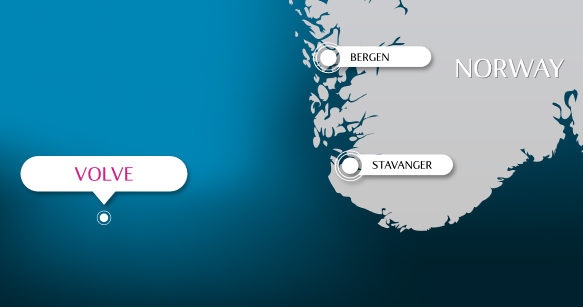
\includegraphics [width=1\linewidth,right]{Volve.jpg}
\end{figure}

\end{columns}

\begin{block}{\ce{Why it is important?}}
\ce{A well-trained model as a powerful tool to support future oil drilling system design and optimization}
\end{block}
\end{frame}


\begin{frame}
\frametitle{Problem Statement}
\begin{columns}[]
\column{.5\textwidth} % Left column and width
\begin{itemize}
\item 23 types of information, covering more than 15000 operation days
\item 12 of them are directly related to our target
\item Prediction on oil production rate based on these features
\end{itemize}
\column{.5\textwidth} % Right column and width
\begin{table}
\begin{tabular}{c}
\toprule
\textbf{Features}\\
\midrule
Date of production\tabularnewline
On-stream hours\tabularnewline
Average downhole pressure\tabularnewline
Average downhole temperature\tabularnewline
Average differential pressure tubing\tabularnewline
Average annulus pressure\tabularnewline
Average choke size\tabularnewline
Average wellhead pressure\tabularnewline
Average wellhead temperature\tabularnewline
Differential pressure at choke\tabularnewline
Production/injection\tabularnewline
Bore water injection volume\tabularnewline
\bottomrule
\end{tabular}
%\caption{Table caption}
\end{table}

\end{columns}
\end{frame}

%------------------------------------------------
\section{Literature Review}
%------------------------------------------------

\begin{frame}
\frametitle{Literature Review}
\begin{itemize}
\item \textbf{Petroleum production prediction}(\small{Thomas, R.S. \emph{et.al.})}:
\begin{enumerate}
\item by analogy
\item volumetric
\item material balance
\item decline curve fitting
\item reservoir simulation
\end{enumerate}
\item Artificial Neural Network (ANN): the most recent method is to estimate production values \small{(Wong, P.M.\emph{et al.})}. 
\item Higher accuracy when compared to other correlation methods and curve estimation methods \small{(Gharbi, R.B.,\emph{et al.})}.
\item Data pre-processing as the most important step in applying the ANN
\end{itemize}
\begin{block}{}
\ce{Dealing with NA's and zeros considering the physical meaning of features}
\end{block}
\end{frame}

%------------------------------------------------

\section{Data Cleansing}

\subsection{Missing Data Ratios} 
%------------------------------------------------


\begin{frame}
\frametitle{Data Cleansing}
\begin{block}{}
\ce{most data scientists spend almost 60\% of their time and effort on data cleansing}
\end{block}

\begin{columns}[]
\column{.5\textwidth} % Left column and width
Oil production rates less than 10:
\begin{figure}
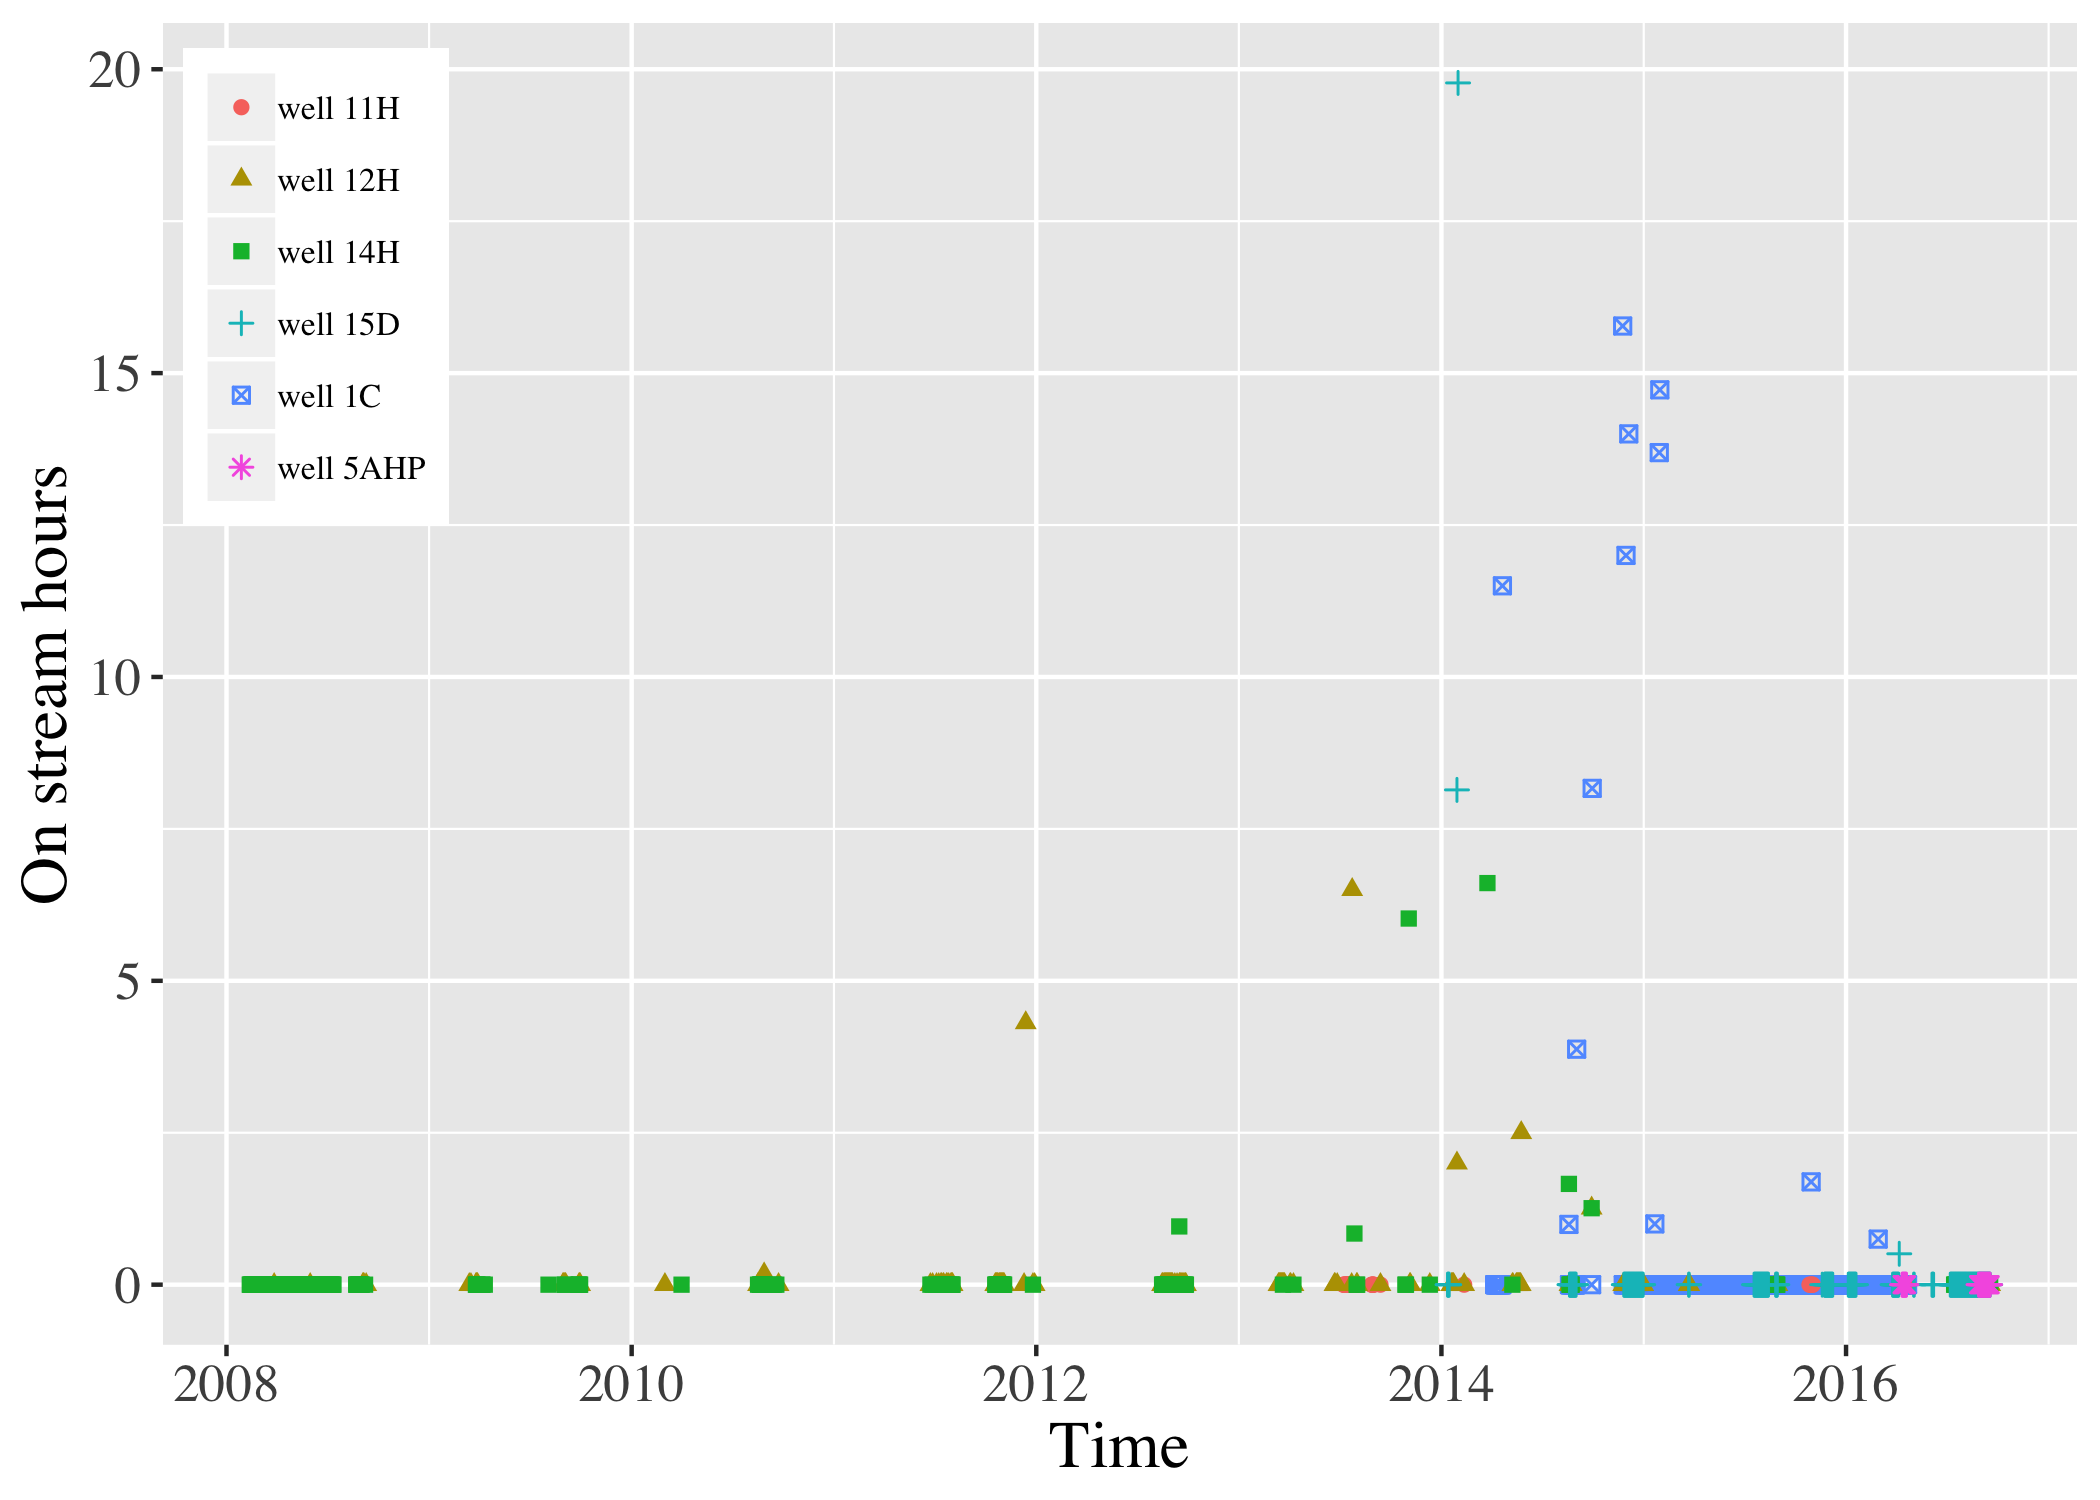
\includegraphics [width=1\linewidth,left]{hrs_t_0.png}
\end{figure}

\column{.5\textwidth} % Right column and width
After removing the oil production rates less than or equal to 10:

\begin{table}
\begin{tabular}{l c c }
\toprule
\textbf{Well code} & \textbf{Type} & \textbf{Size}\\
\midrule
12H& production & 2832\tabularnewline
14H&production& 2718\tabularnewline
11H& production& 1123\ \tabularnewline
15D& production& 766\tabularnewline
1C&  production & 426  \tabularnewline
5AHP&production& 129 \tabularnewline
4AH & injection & 3327\tabularnewline
5AHI & injection & 3146 \tabularnewline
\bottomrule
\end{tabular}
%\caption{Table caption}
\end{table}
\end{columns}

\end{frame}


\begin{frame}
\frametitle{Data Cleansing - Missing Data Ratios}
\begin{block}{}
Missing data ratios of production wells:
\end{block}
\begin{table}
\begin{adjustbox}{width=1\linewidth,center}
\begin{tabular}{lcccccc}
\toprule
\textbf{Feature}&\textbf{Well 1C}&\textbf{Well 11H}&\textbf{Well 12H}&\textbf{Well 14H}&\textbf{Well 15D}&\textbf{Well 5AHP}\tabularnewline
\midrule
Avg. annulus pressure&\cellcolor{red!70}100\% & 0.53\% & 0.46\% & \cellcolor{red!70}49.6\% & --- & --- \tabularnewline
Avg. downhole pressure& --- & 0.45\%& \cellcolor{red!70}67.4 \% & 0.77\% & --- &\cellcolor{red!25}100\% \tabularnewline
Avg. downhole temperature& --- & 0.45\%& \cellcolor{red!70}67.4\% & 0.77\% & ---&\cellcolor{red!25}100\%\tabularnewline
Avg. $\Delta$P tubing& ---& 0.45\%&0.21\% & 0.22\% & ---&\cellcolor{red!25}100\% \tabularnewline
Avg. well head pressure& ---& 0.45\% & 0.04\% & 0.04\% & ---& ---\tabularnewline
Avg. well head temperature&---& 0.45\% & --- & --- & ---  & ---\tabularnewline
$\Delta$P chock size &---& 0.45\%& --- & --- & ---& ---\tabularnewline
On-stream hours &---& 0.09\%& --- & --- & ---& ---\tabularnewline
\bottomrule
\end{tabular}
\end{adjustbox}
\end{table}
\begin{block}{}
For injection wells: \\ 14.14\% of water injection volume for well 5AHI \\ 10.13\% of water injection volume for well 4AH
\end{block}
\end{frame}



%------------------------------------------------
\subsection{Removing Outliers } 
%------------------------------------------------

\begin{frame}
\frametitle{Data Cleansing - Removing Outliers}
\begin{block}{}
After using z-score with a threshold equals to 3 to drop the outliers:
\end{block}
\begin{table}
\begin{center}
\begin{tabular}{lcc}
\toprule
\textbf{Well code}&\textbf{Type}&\textbf{Outlier percentage}\tabularnewline
\midrule
Well 12H& production & 5.1\%\tabularnewline
Well 14H&production& 6.5\% \tabularnewline
Well 11H& production& 1.8\%\ \tabularnewline
Well 15D& production& 8.3\% \tabularnewline
Well 1C&  production & 7\%  \tabularnewline
Well 4AH & injection & no outlier\tabularnewline
Well 5AHI & injection & no outlier \tabularnewline
\bottomrule
\end{tabular}\end{center}
\end{table}

\end{frame}

%------------------------------------------------
\subsection{Data Imputation} 
%------------------------------------------------


\begin{frame}
\frametitle{Data Cleansing - Missing Data Imputation}
\begin{block}{}
Some visual inspections on features...
\end{block}
\begin{columns}[c]
\column{.5\textwidth} % Left column and width

\begin{figure}
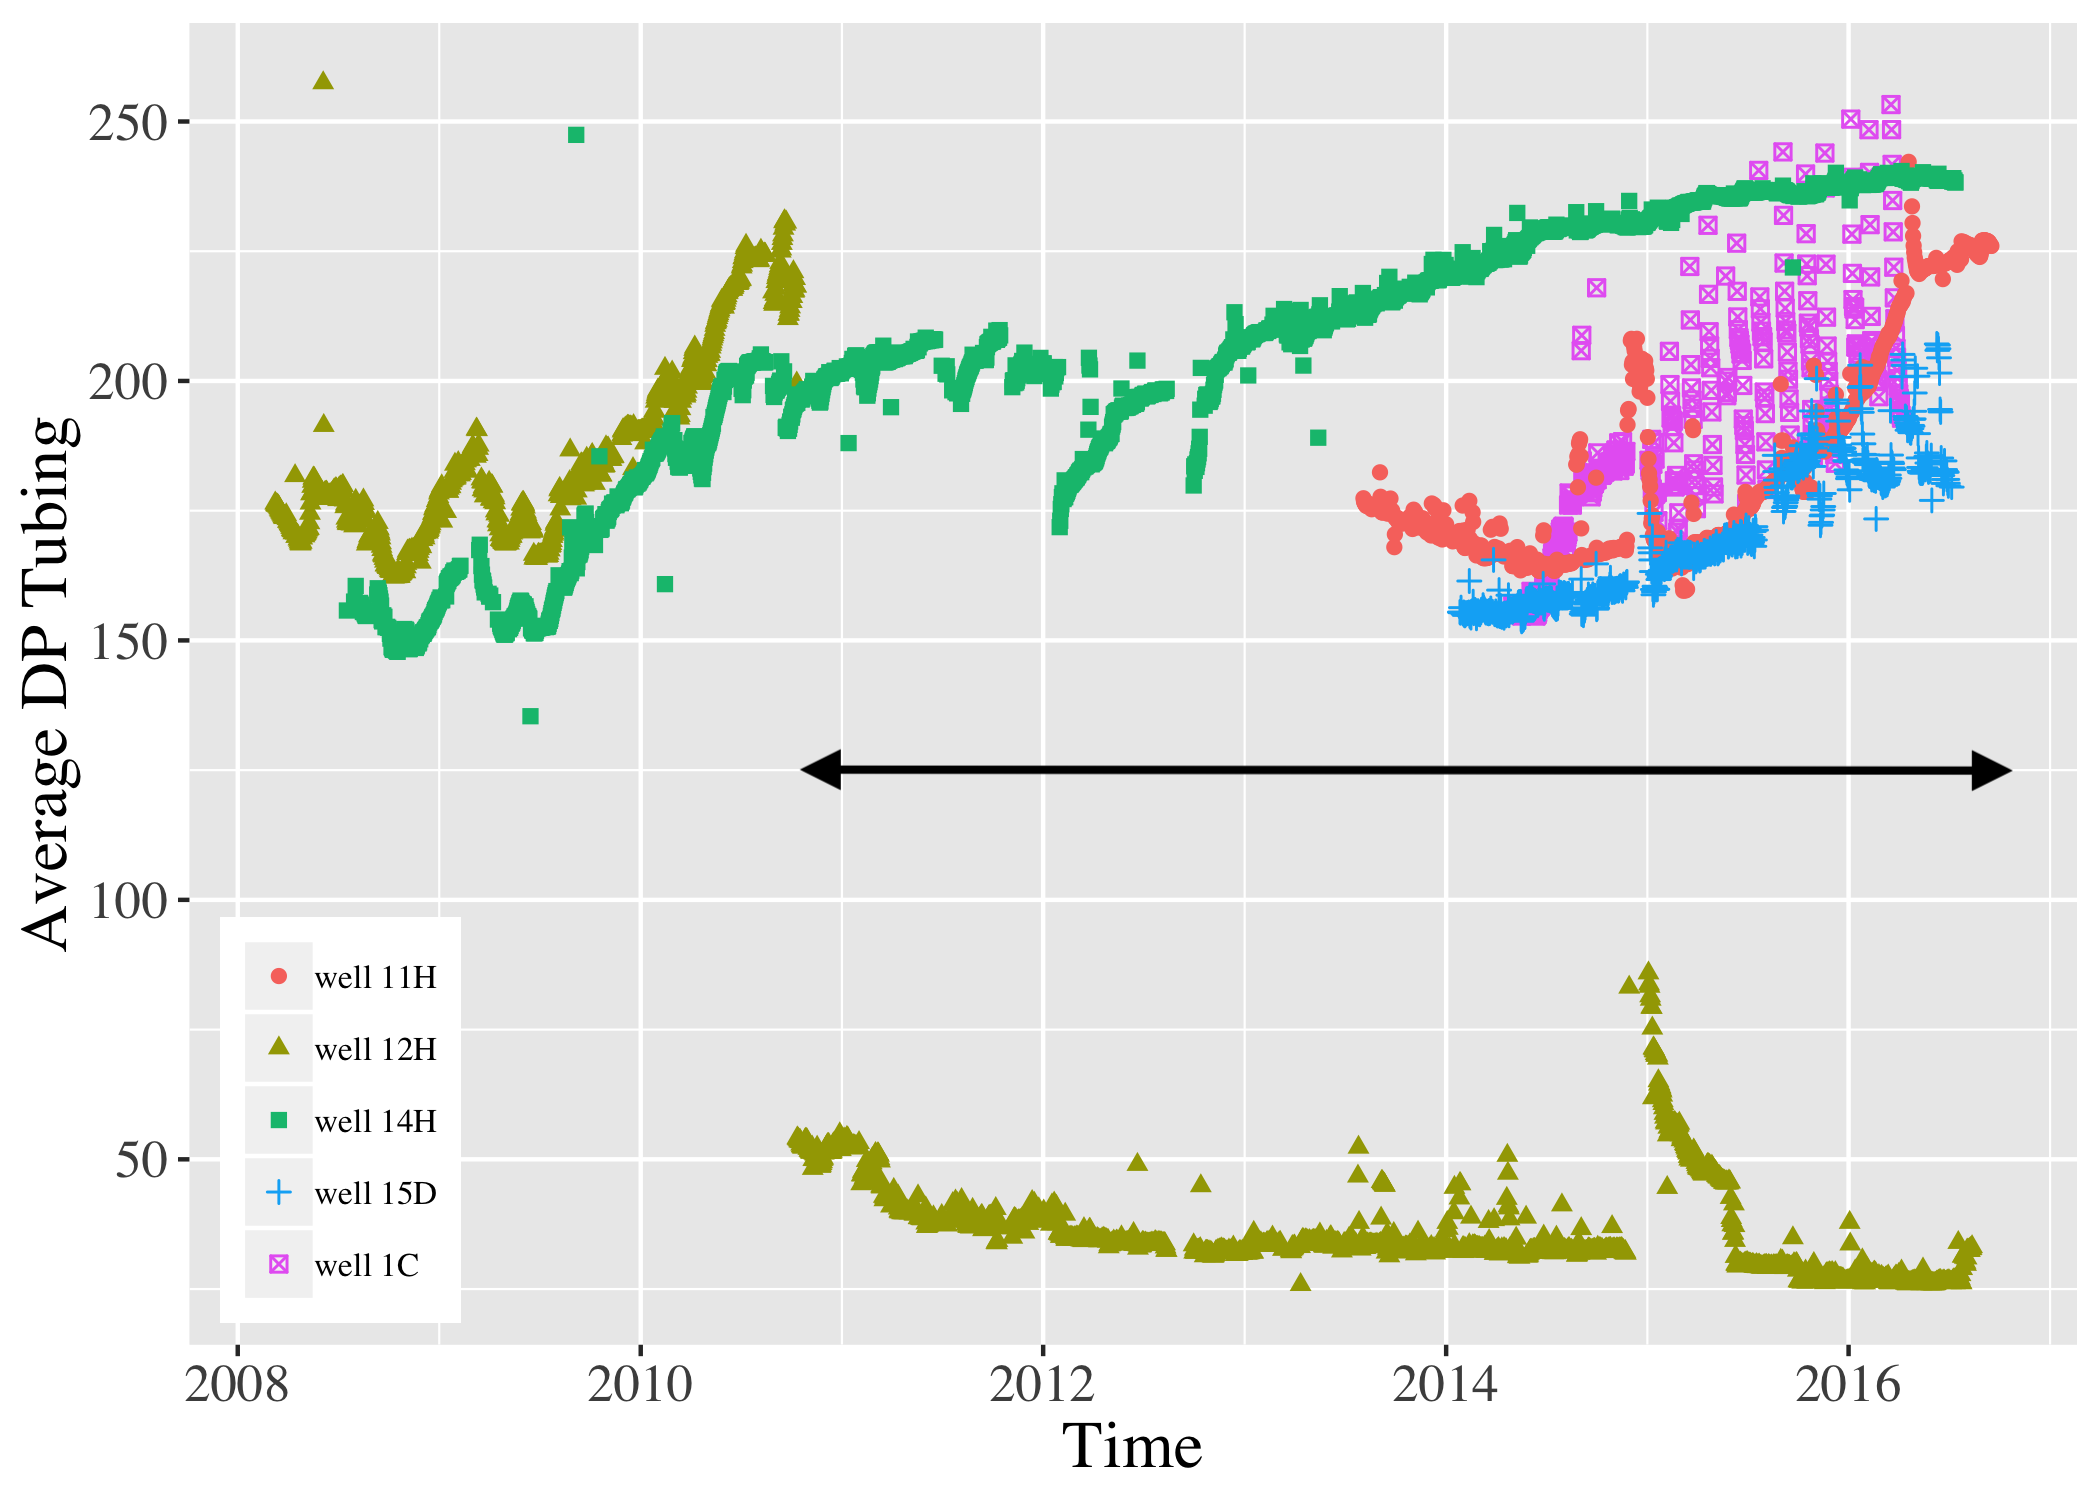
\includegraphics[width=1\linewidth,left]{adpt_t.png} 
\end{figure}

\column{.5\textwidth} % Right column and width
\begin{figure}
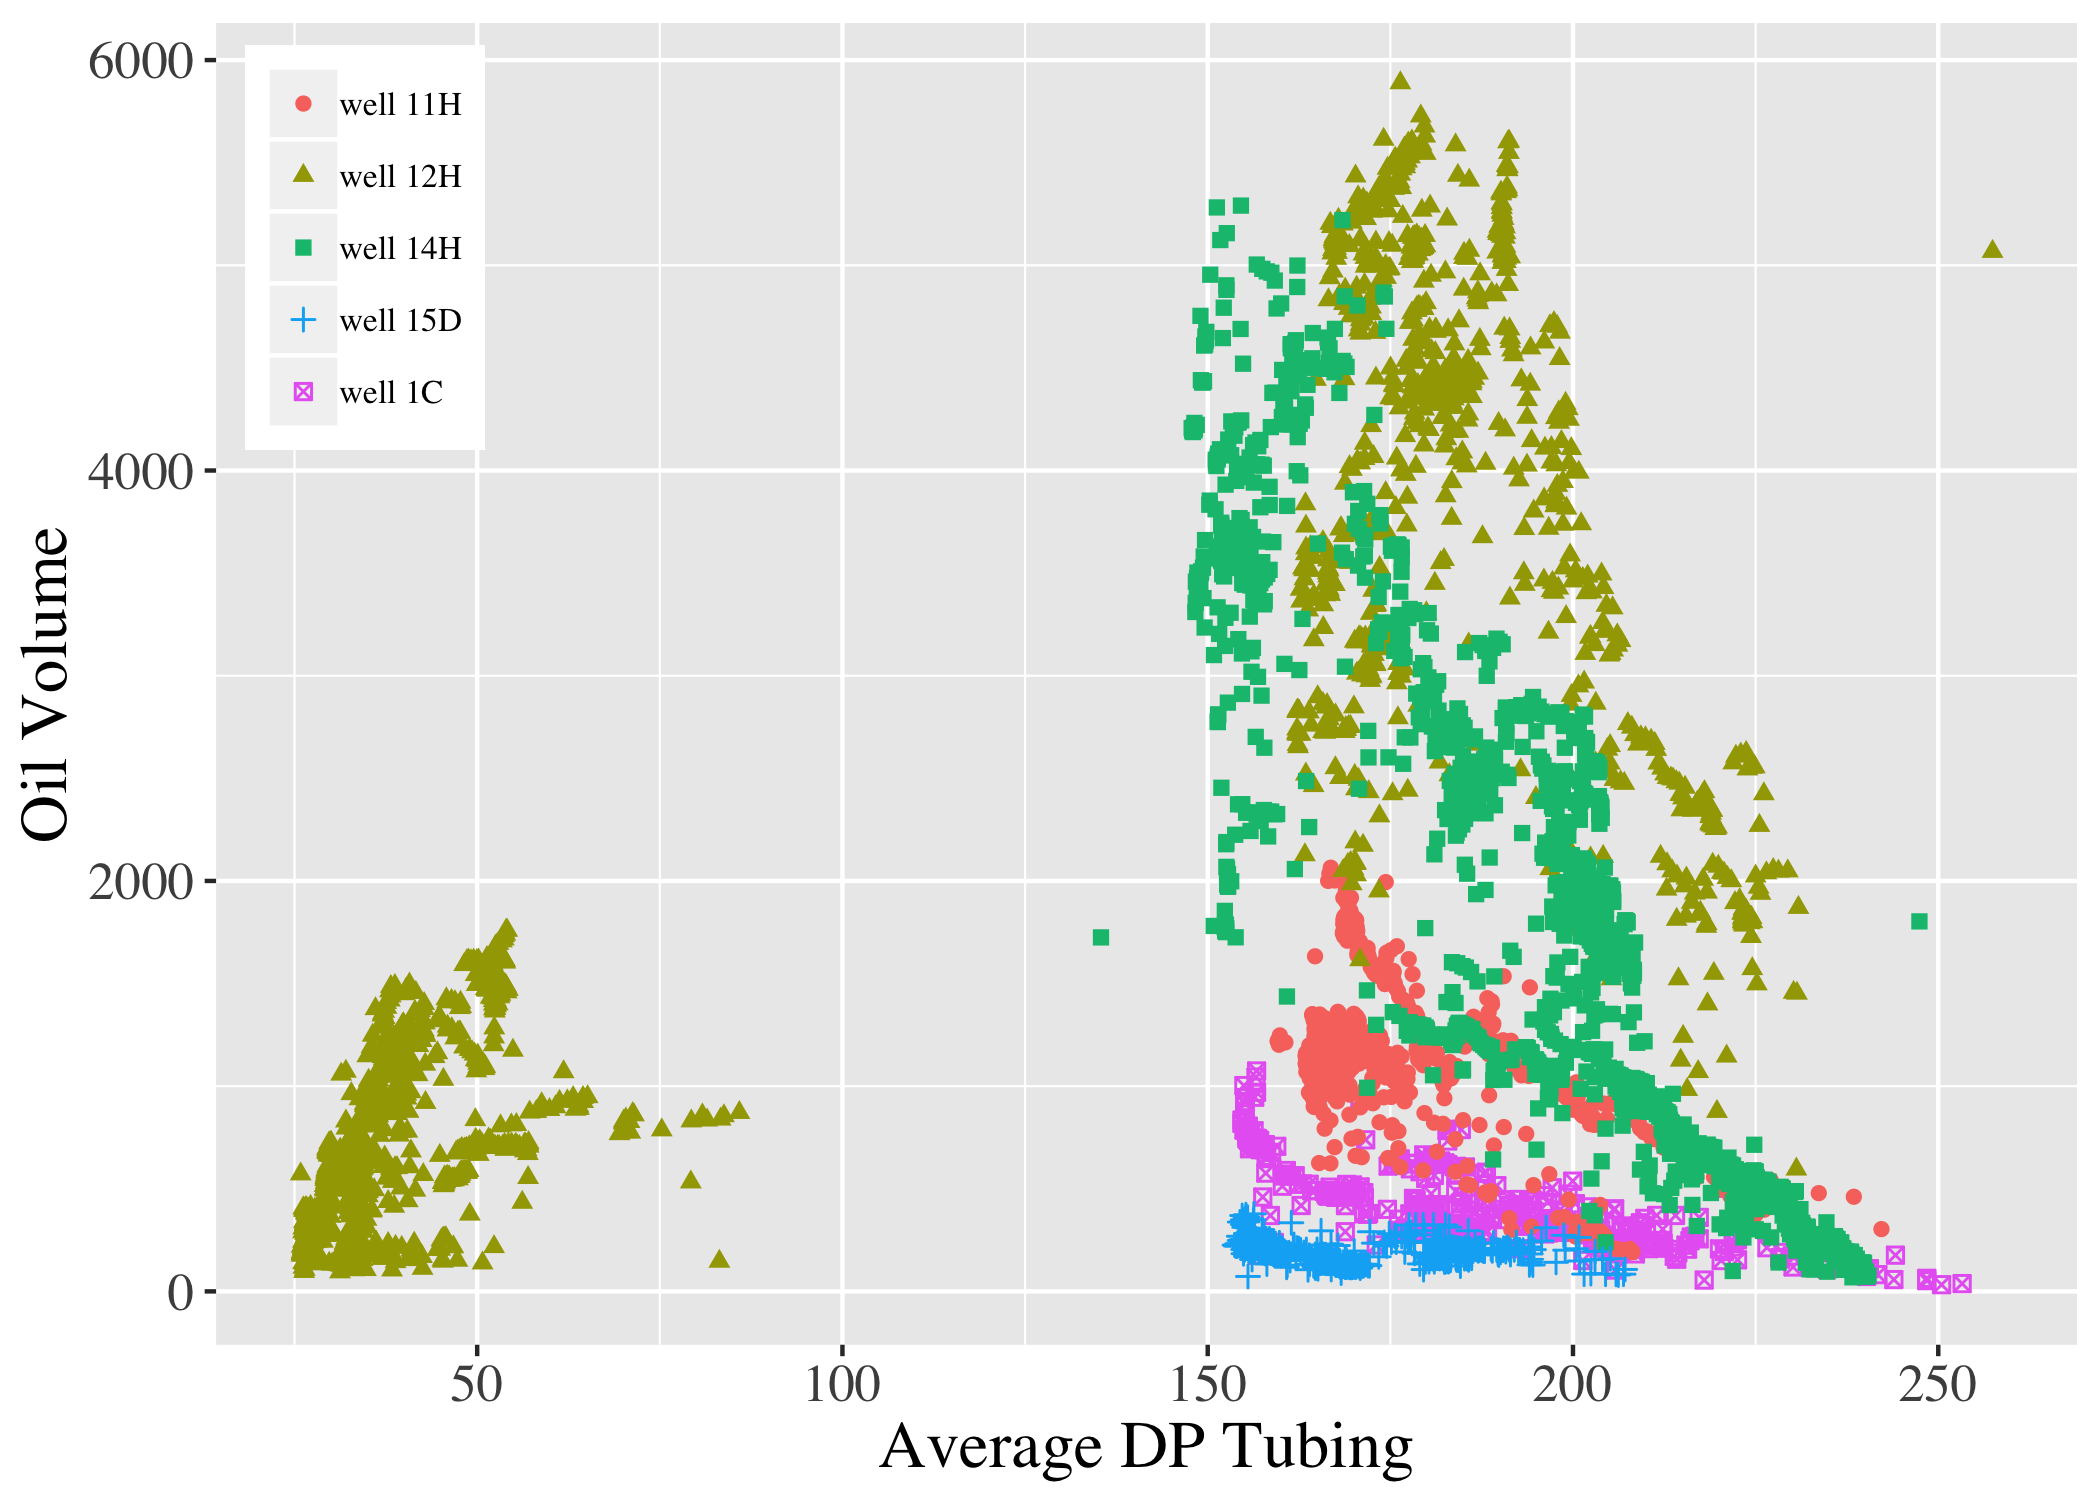
\includegraphics[width=1\linewidth, right]{o_adpt.png}
\end{figure}
\end{columns}

\begin{block}{}
The values less than 100 will be replaced with NA's
\end{block}
\end{frame}


\begin{frame}
\frametitle{Data Cleansing - Missing Data Imputation}
\begin{block}{}
Some visual inspections on features...
\end{block}
\begin{columns}[c]
\column{.5\textwidth} % Left column and width

\begin{figure}
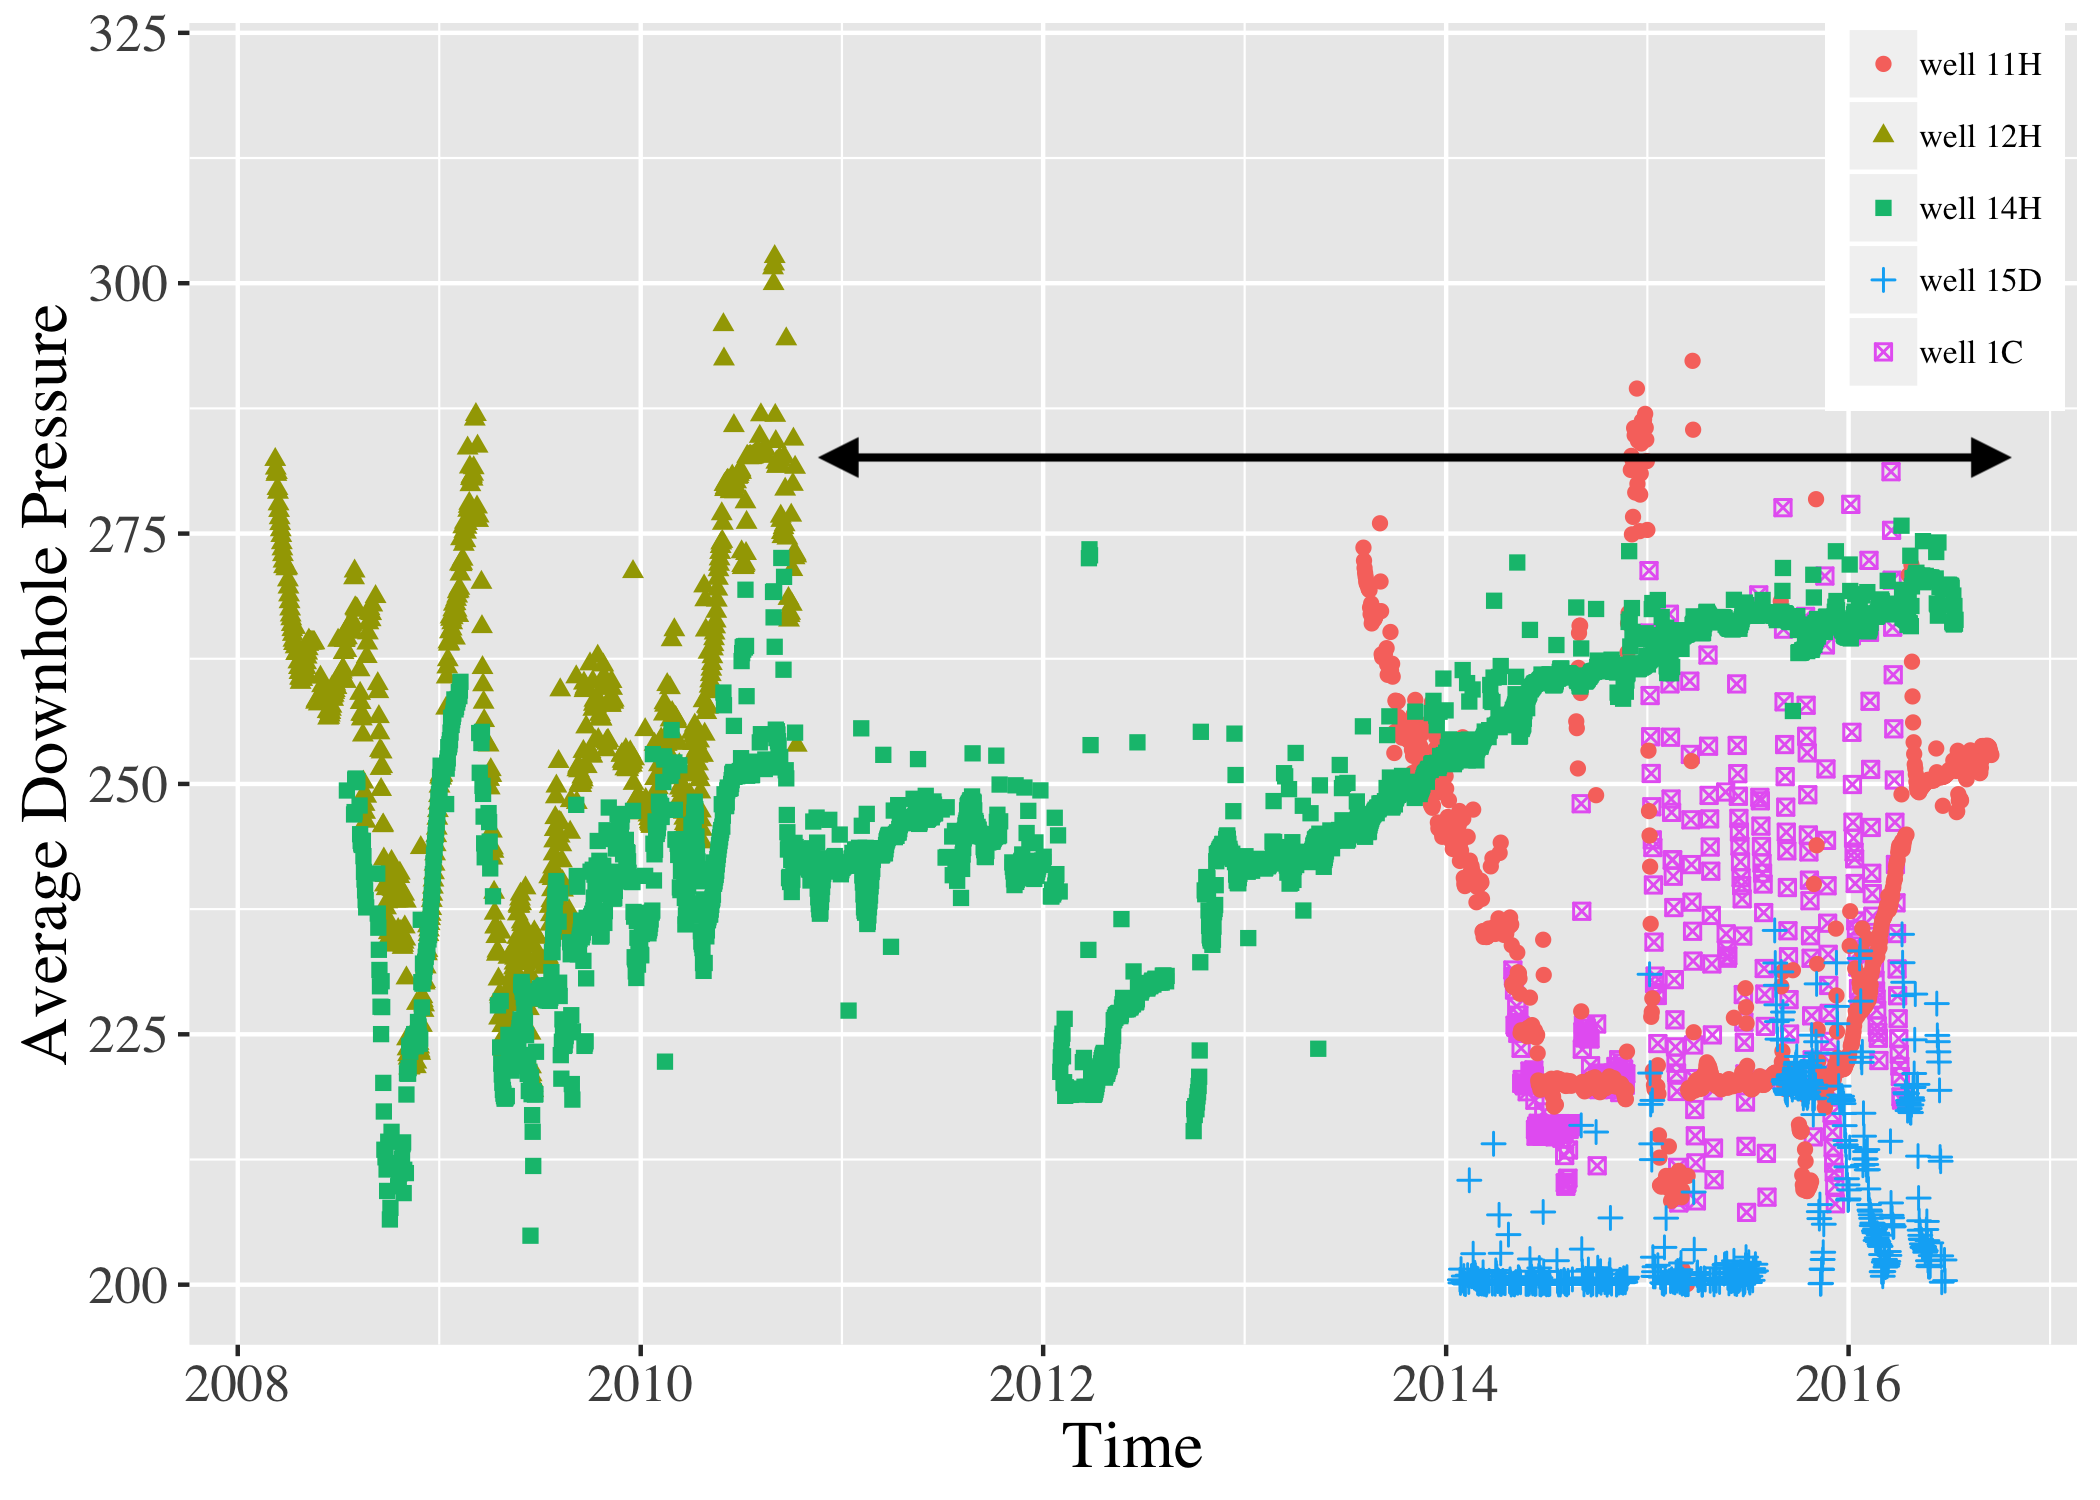
\includegraphics[width=1\linewidth,left]{adp_t_copy.png} 
\end{figure}

\column{.5\textwidth} % Right column and width
\begin{figure}
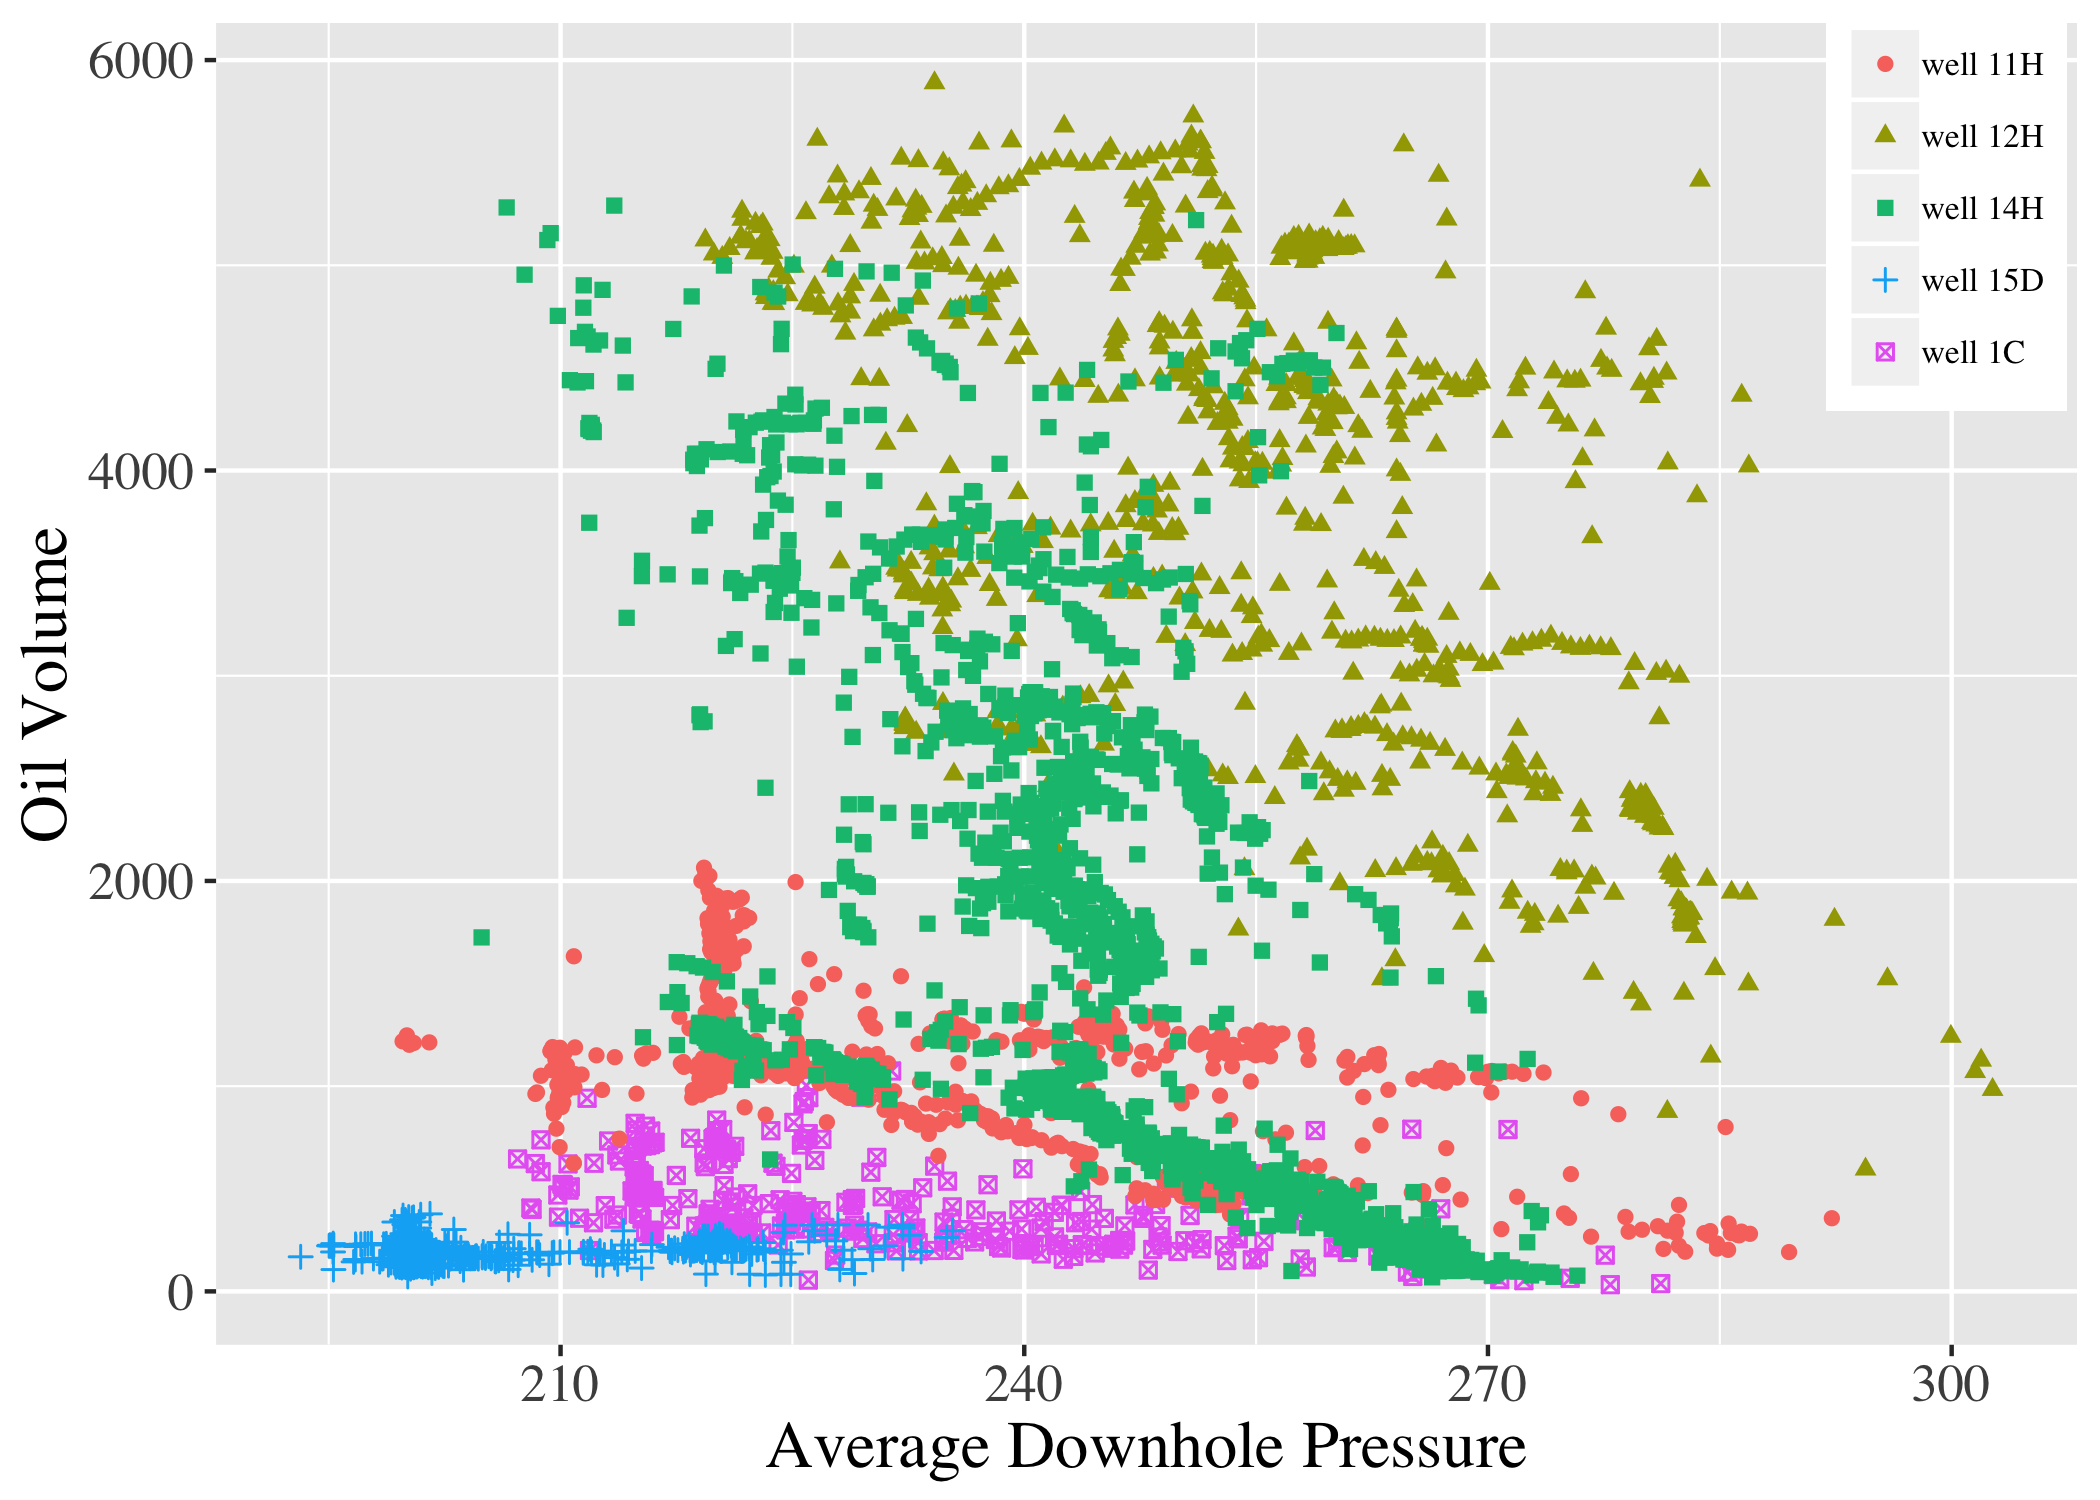
\includegraphics[width=1\linewidth, right]{o_adp.png}
\end{figure}
\end{columns}

\begin{block}{}
The values in the shown time range will be imputed
\end{block}
\end{frame}

\begin{frame}
\frametitle{Data Cleansing - Missing Data Imputation}
\begin{block}{}
Some visual inspections on features...
\end{block}
\begin{columns}[c]
\column{.5\textwidth} % Left column and width

\begin{figure}
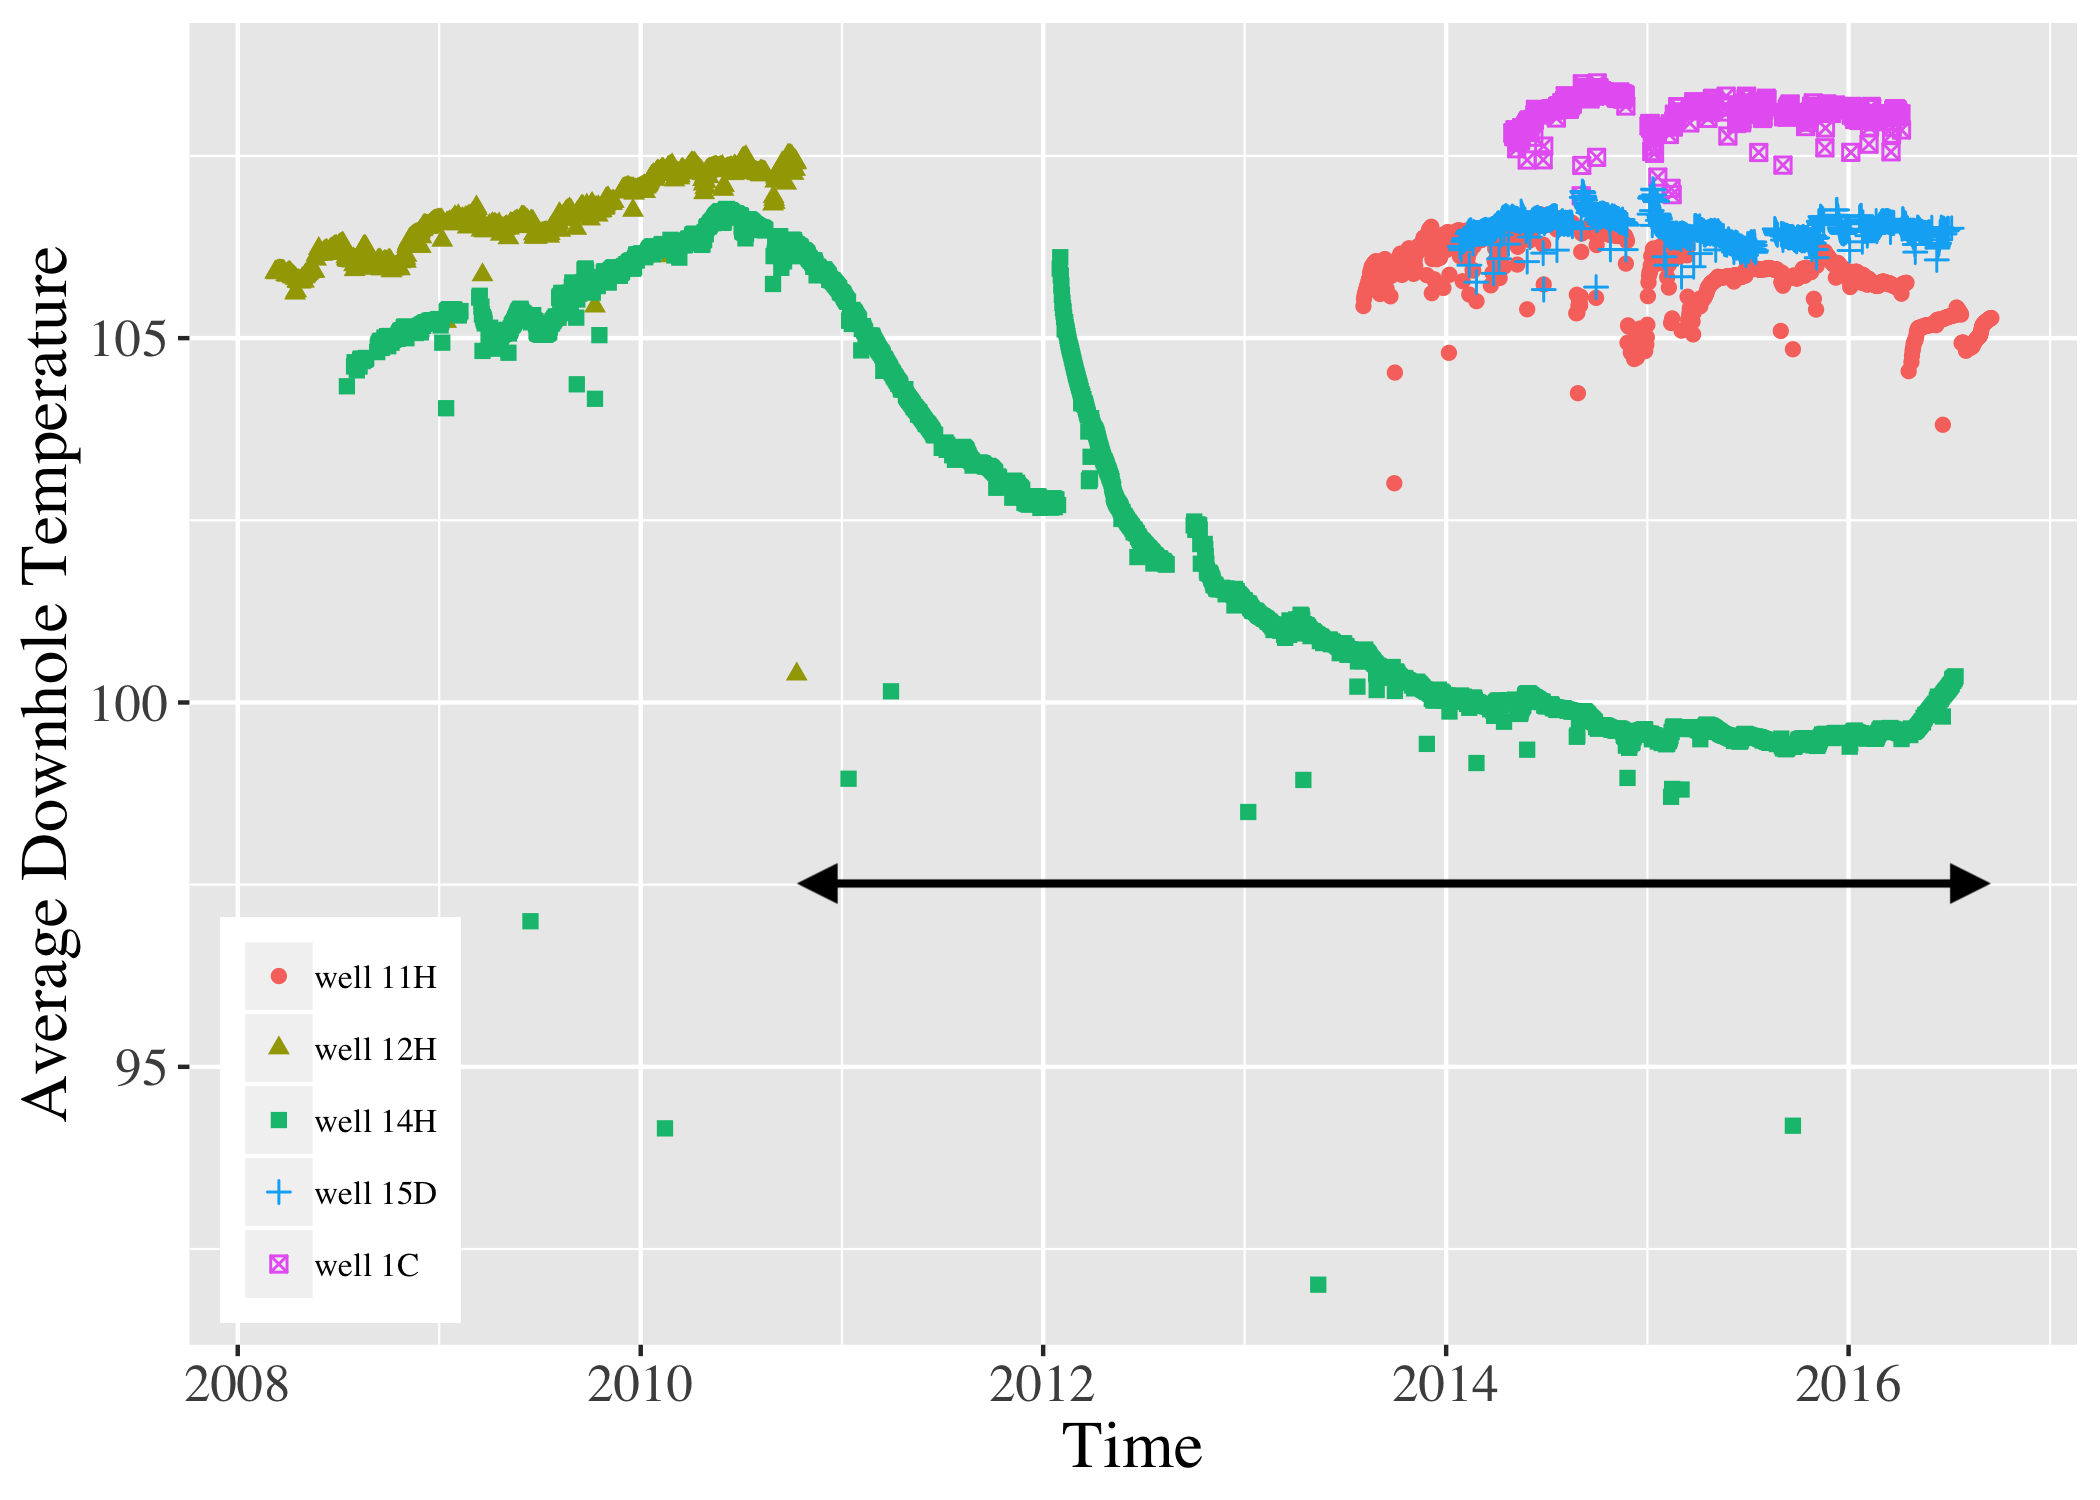
\includegraphics[width=1\linewidth,left]{adt_t_copy.png} 
\end{figure}

\column{.5\textwidth} % Right column and width
\begin{figure}
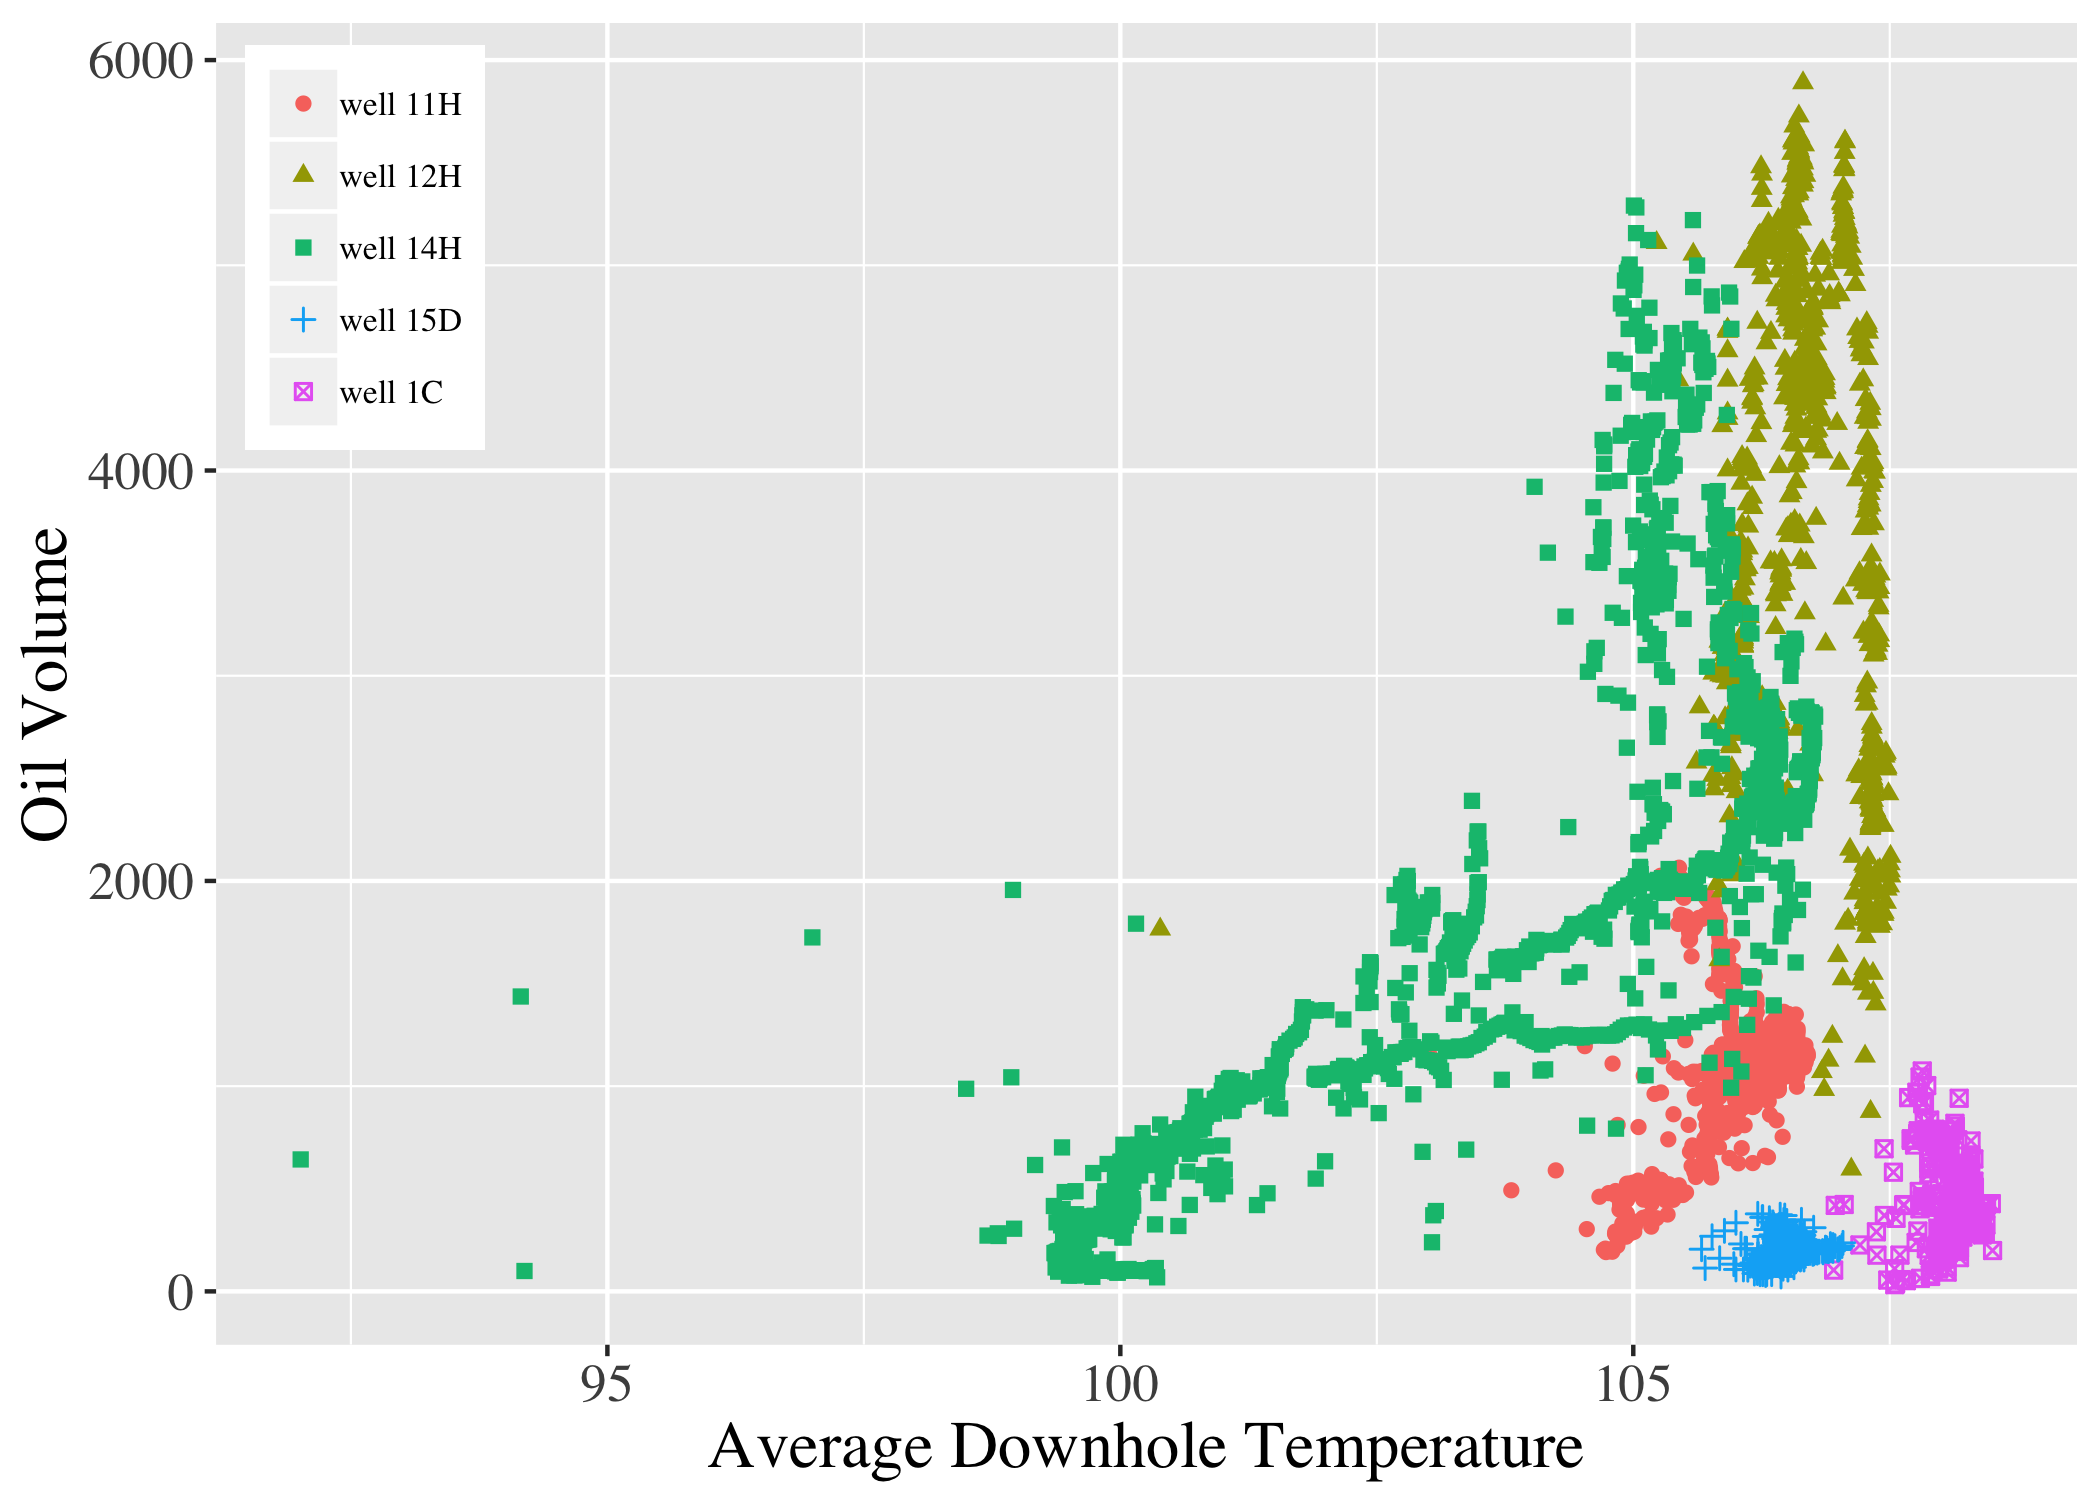
\includegraphics[width=1\linewidth, right]{o_adt.png}
\end{figure}
\end{columns}

\begin{block}{}
The values in the shown time range will be imputed
\end{block}
\end{frame}

\begin{frame}
\frametitle{Data Cleansing - Missing Data Imputation}
\begin{block}{}
Some visual inspections on features...
\end{block}
\begin{columns}[c]
\column{.5\textwidth} % Left column and width

\begin{figure}
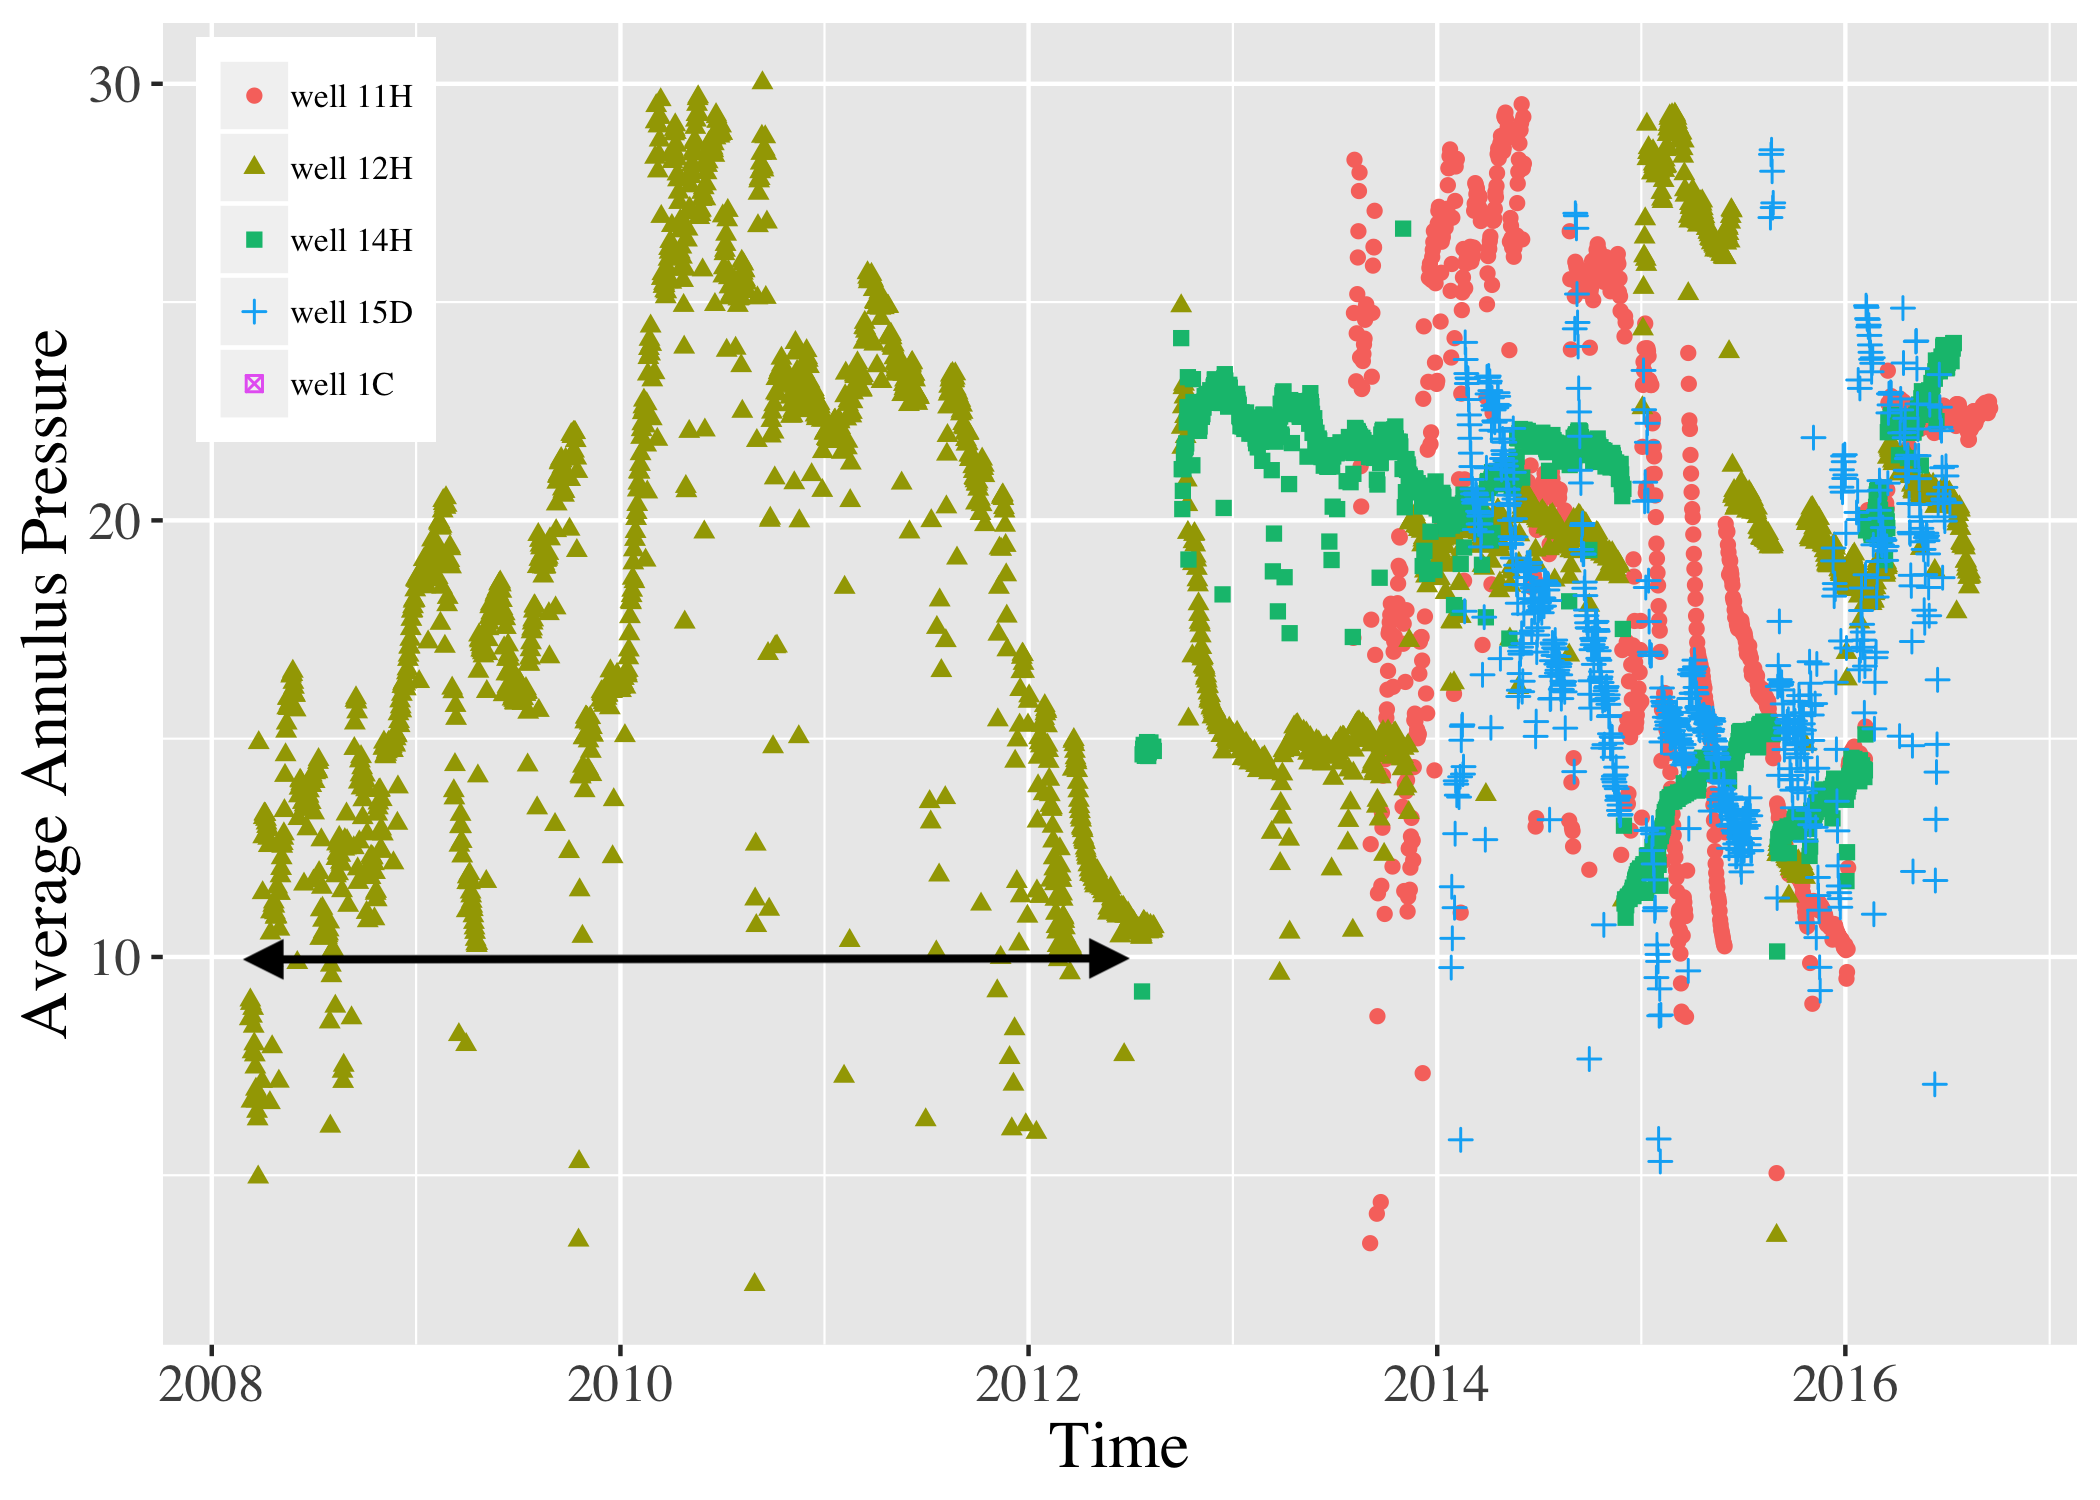
\includegraphics[width=1\linewidth,left]{aap_t_copy.png} 
\end{figure}

\column{.5\textwidth} % Right column and width
\begin{figure}
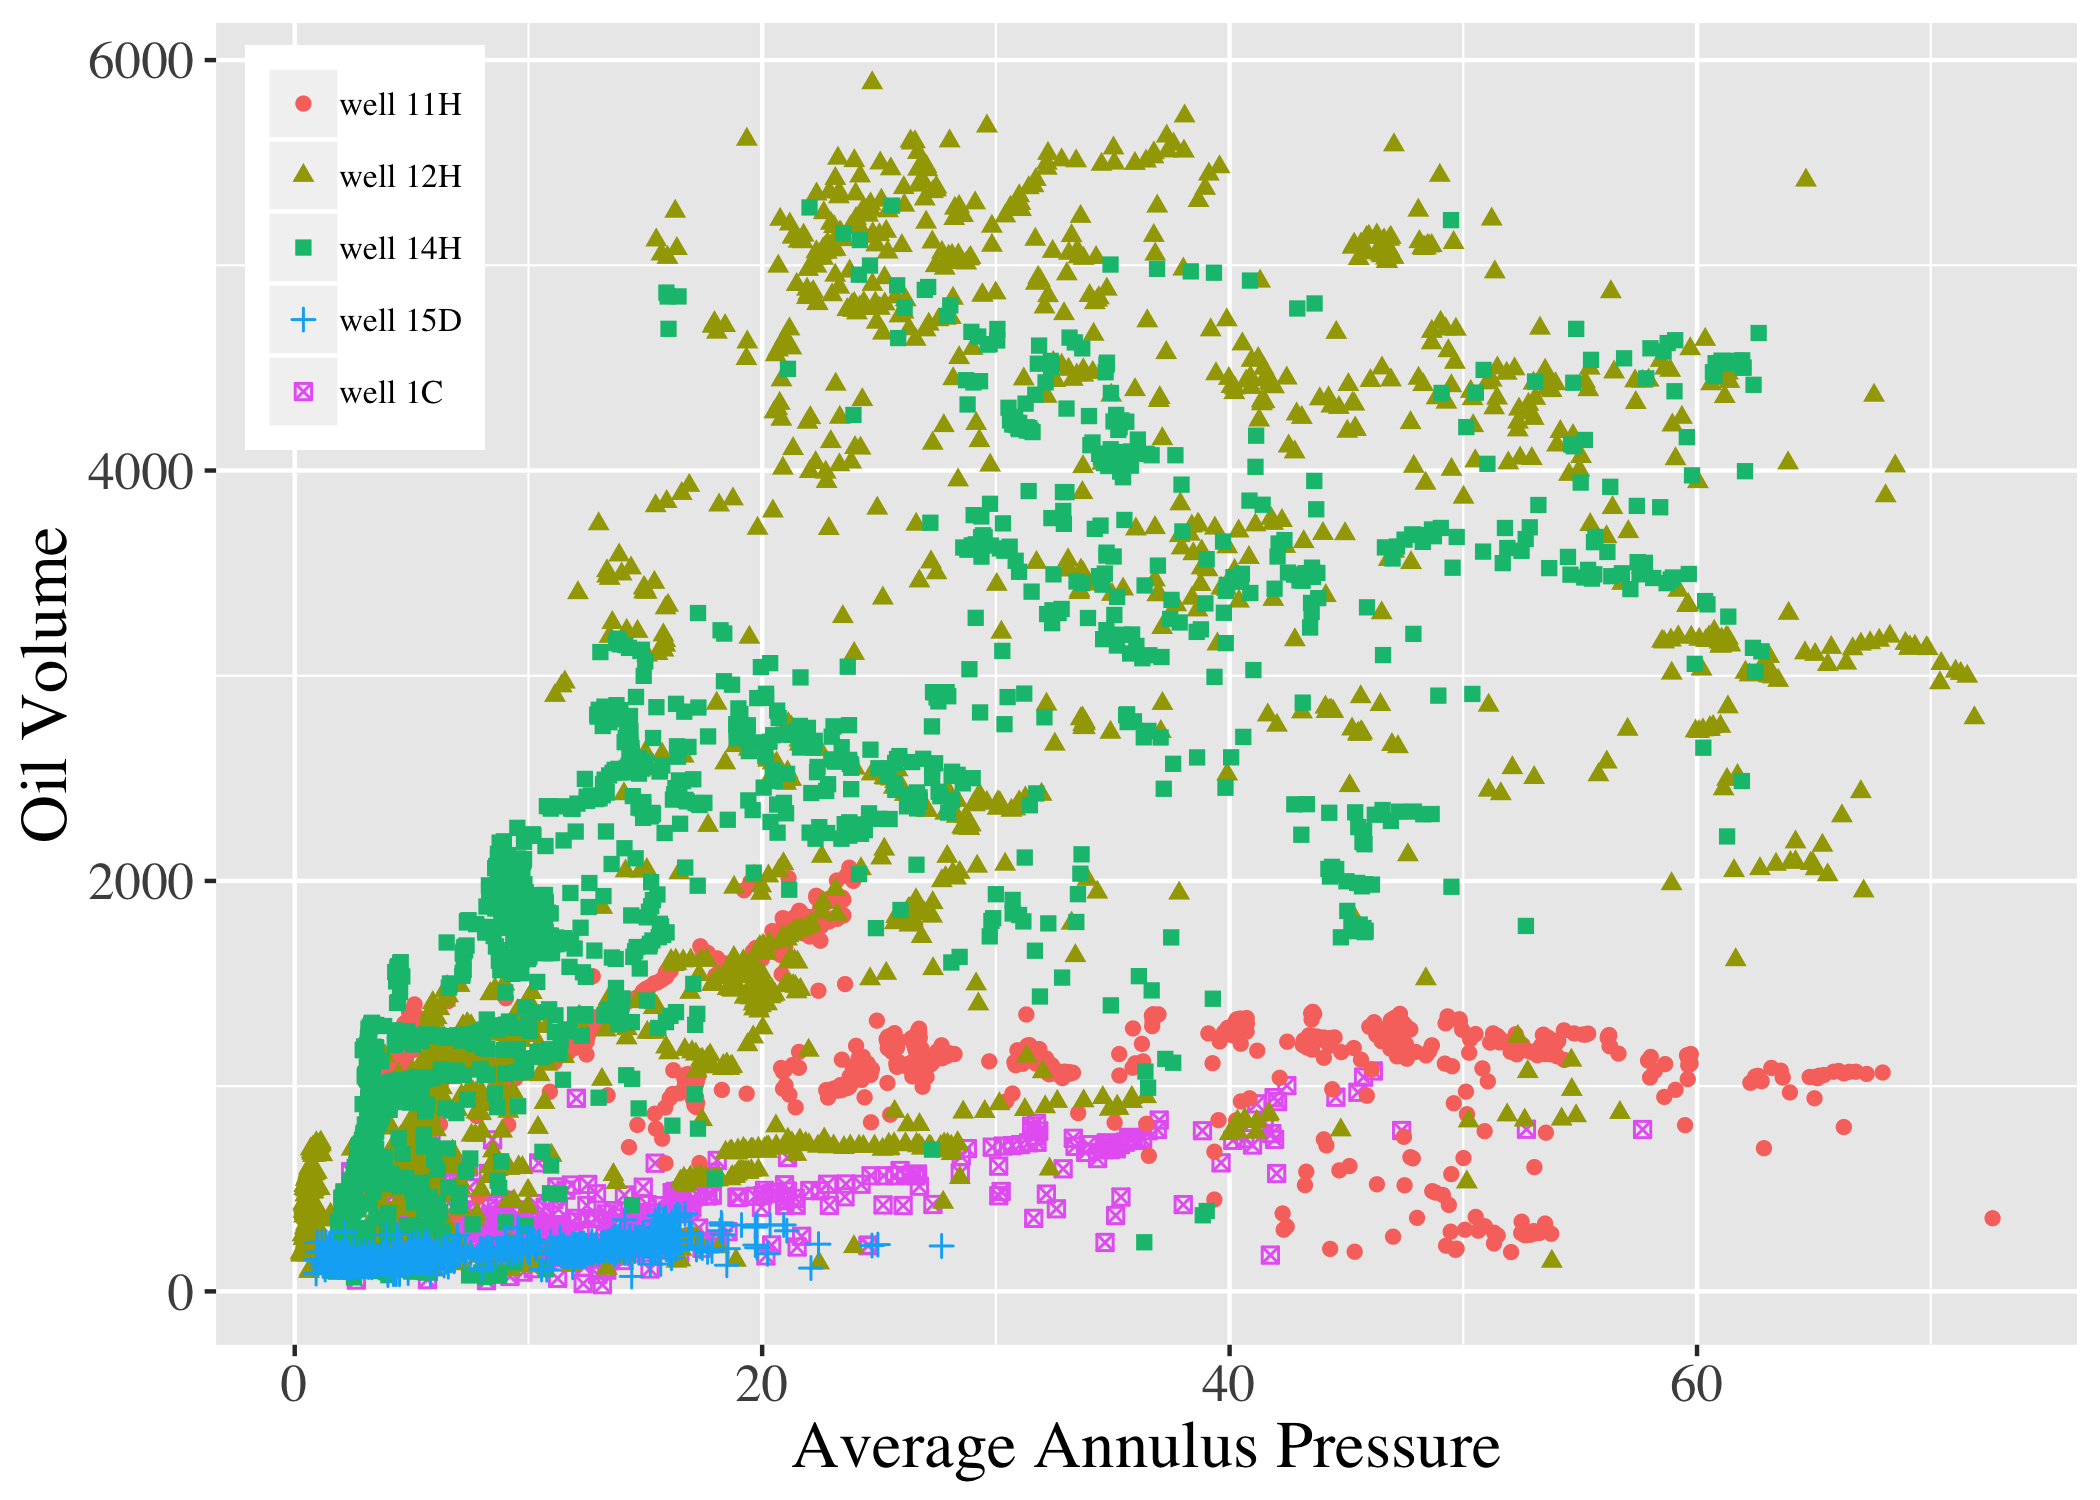
\includegraphics[width=1\linewidth, right]{o_aap.png}
\end{figure}
\end{columns}

\begin{block}{}
The values in the shown time range will be imputed
\end{block}
\end{frame}


\begin{frame}
\frametitle{Data Cleansing - Missing Data Imputation}
\textbf{Missing data values which need to be imputed:}
\begin{enumerate}
\item Water injection volume for well 5AHI and 4AHI using Kalman Filter
\item Avg. $\Delta$P tubing for well 14H using SVR and MLP model
\item Avg. downhole pressure and temperature for well 12H using SVR and MLP model
\item Avg. annulus pressure for well 1C and 14H using SVR and MLP model
\end{enumerate}

\end{frame}

\begin{frame}
\frametitle{Data Cleansing - Missing Data Imputation}
\textbf{Imputation of water injection missing values of well 4AH using Kalman Filter:}
\begin{columns}[c]
\column{.5\textwidth} % Left column and width
\begin{figure}
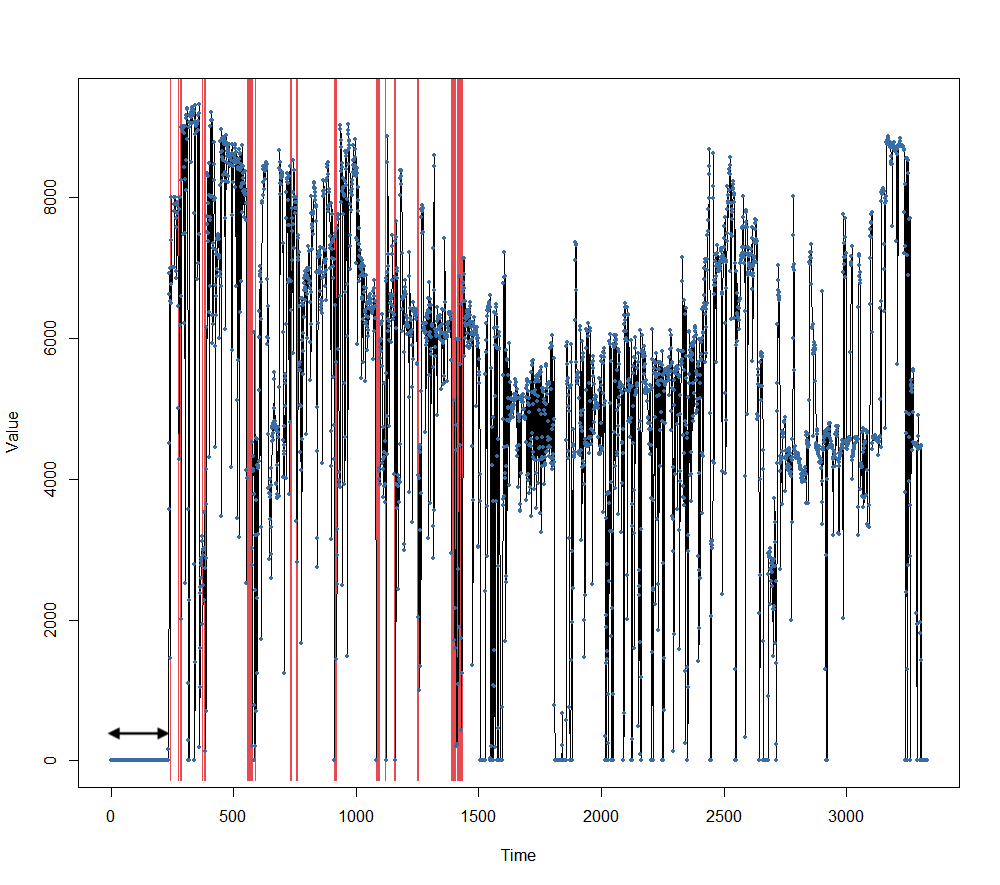
\includegraphics[width=1\linewidth,left]{WI_missing1.png} 
\end{figure}


\column{.5\textwidth} % Right column and width
\begin{figure}
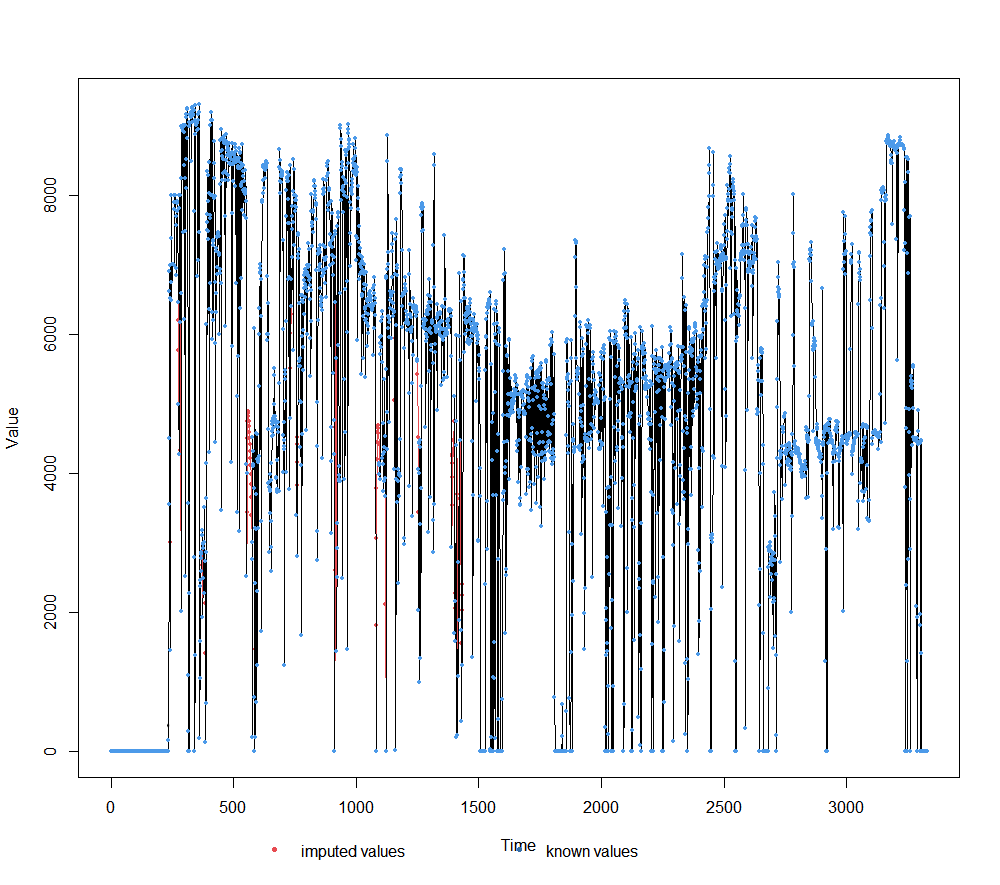
\includegraphics[width=1\linewidth,left]{WI_imputation1.png} 
\end{figure}


\end{columns}

\end{frame}



\begin{frame}
\frametitle{Data Cleansing - Missing Data Imputation}
\textbf{Imputation of water injection missing values of well 5AHI using ARIMA:}
\begin{columns}[c]
\column{.5\textwidth} % Left column and width

\begin{figure}
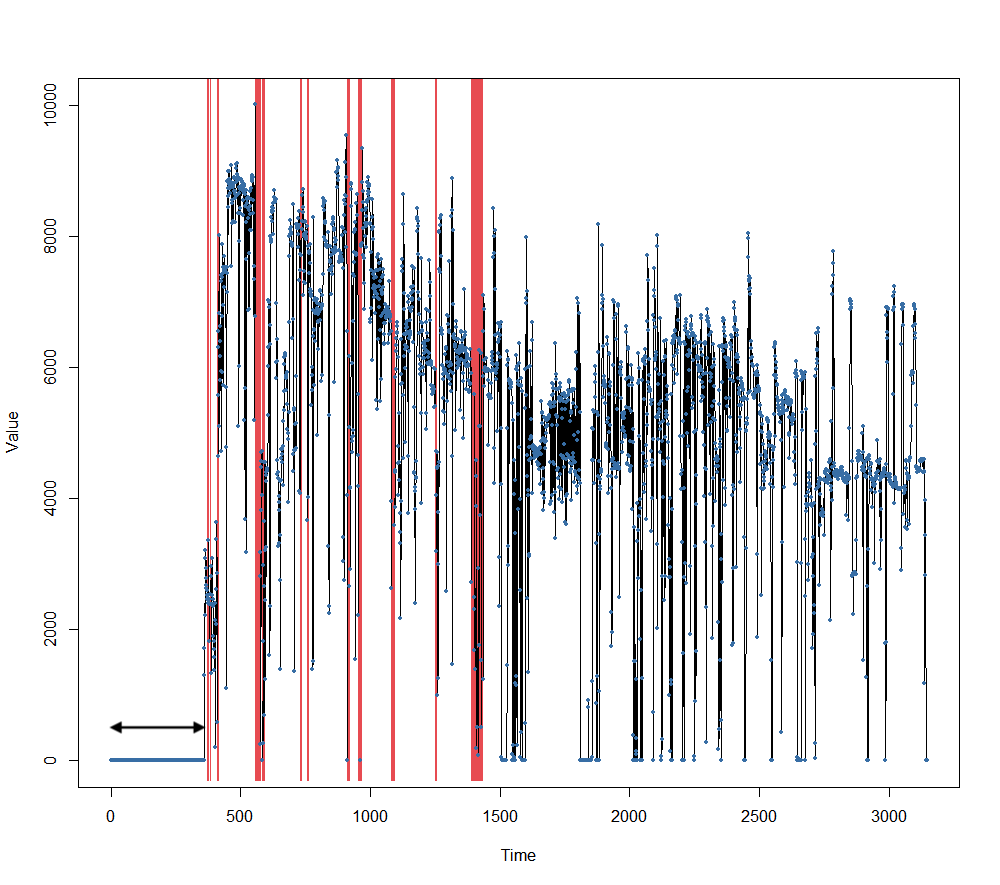
\includegraphics[width=1\linewidth,left]{WI_missing2.png} 
\end{figure}

\column{.5\textwidth} % Right column and width

\begin{figure}
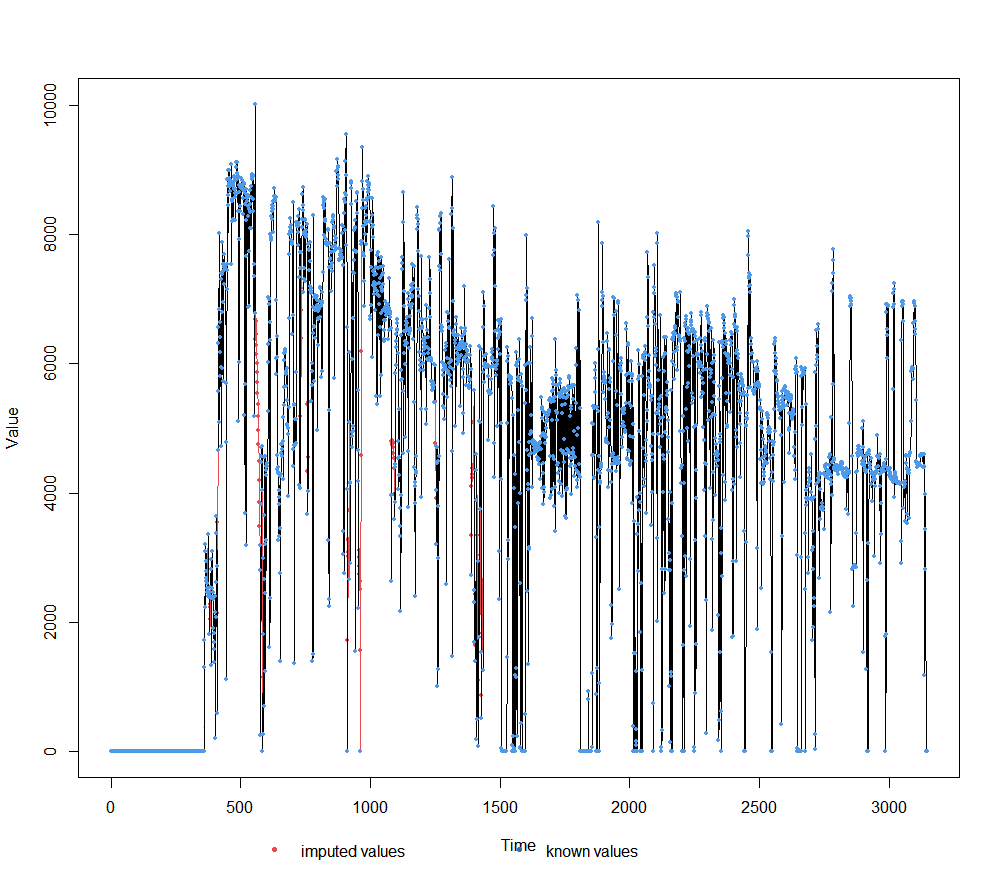
\includegraphics[width=1\linewidth,left]{WI_imputation2.png} 
\end{figure}

\end{columns}
\end{frame}


\begin{frame}
\frametitle{Data Cleansing - Missing Data Imputation}
\textbf{Results of imputation using SVR and MLP:}
\begin{itemize}
\item Order of imputation
\item Using all available non-missing features/data from all wells 
\item Splitting the dataset into two training (80\%) and test (20\%) sets
\item Cross-validation with 10 fold in training set
\item Grid search for \emph{cost} and \emph{sigma} values (from 4 up to 7 values for each)
\end{itemize}

\begin{table}
\begin{adjustbox}{width=1\linewidth,center}
\label{tb:rs_adpt}
\begin{tabular}{lccccccc}
\toprule
\textbf{Imputed feature}&\textbf{Model}&\textbf{R-squared}&\textbf{RMSE}&\textbf{Sigma}&\textbf{Cost}&\textbf{Layer \& Neurons}&\textbf{Epochs}\tabularnewline
\midrule
Avg. $\Delta$P tubing & SVR &\cellcolor{green!40}0.90 & 8.00 & 3 & 8 & ---&---\tabularnewline
Avg. $\Delta$P tubing & MLP & 0.91 & 0.308 & --- & --- & [32, 16] & 100 \tabularnewline
Avg. downhole pressure & SVR&\cellcolor{green!40}0.89 & 7.44 & 5 & 6 & ---&---\tabularnewline
Avg. downhole temperature & SVR&\cellcolor{green!40}0.94 & 0.63 & 5 & 3 & ---&---\tabularnewline
Avg. downhole pressure & MLP & 0.86 & 0.37& --- & --- & [32, 16] & 100\tabularnewline
Avg. downhole temperature & MLP &0.95  & 0.23 & --- & --- &[32, 16] & 100\tabularnewline
Avg. annulus pressure & SVR &\cellcolor{green!40}0.77 & 2.30 & 5 & 20 & ---&--- \tabularnewline
Avg. annulus temperature & MLP &0.74  & 0.50 & --- & --- & [64, 32] & 200 \tabularnewline

\bottomrule
\end{tabular}
\end{adjustbox}
\end{table}

\end{frame}

\begin{frame}
\frametitle{Data Cleansing - Missing Data Imputation}
\begin{block}{}
Some visual inspections on features before and after missing data imputation
\end{block}

\begin{columns}[c]
\column{.5\textwidth} % Left column and width
\begin{figure}
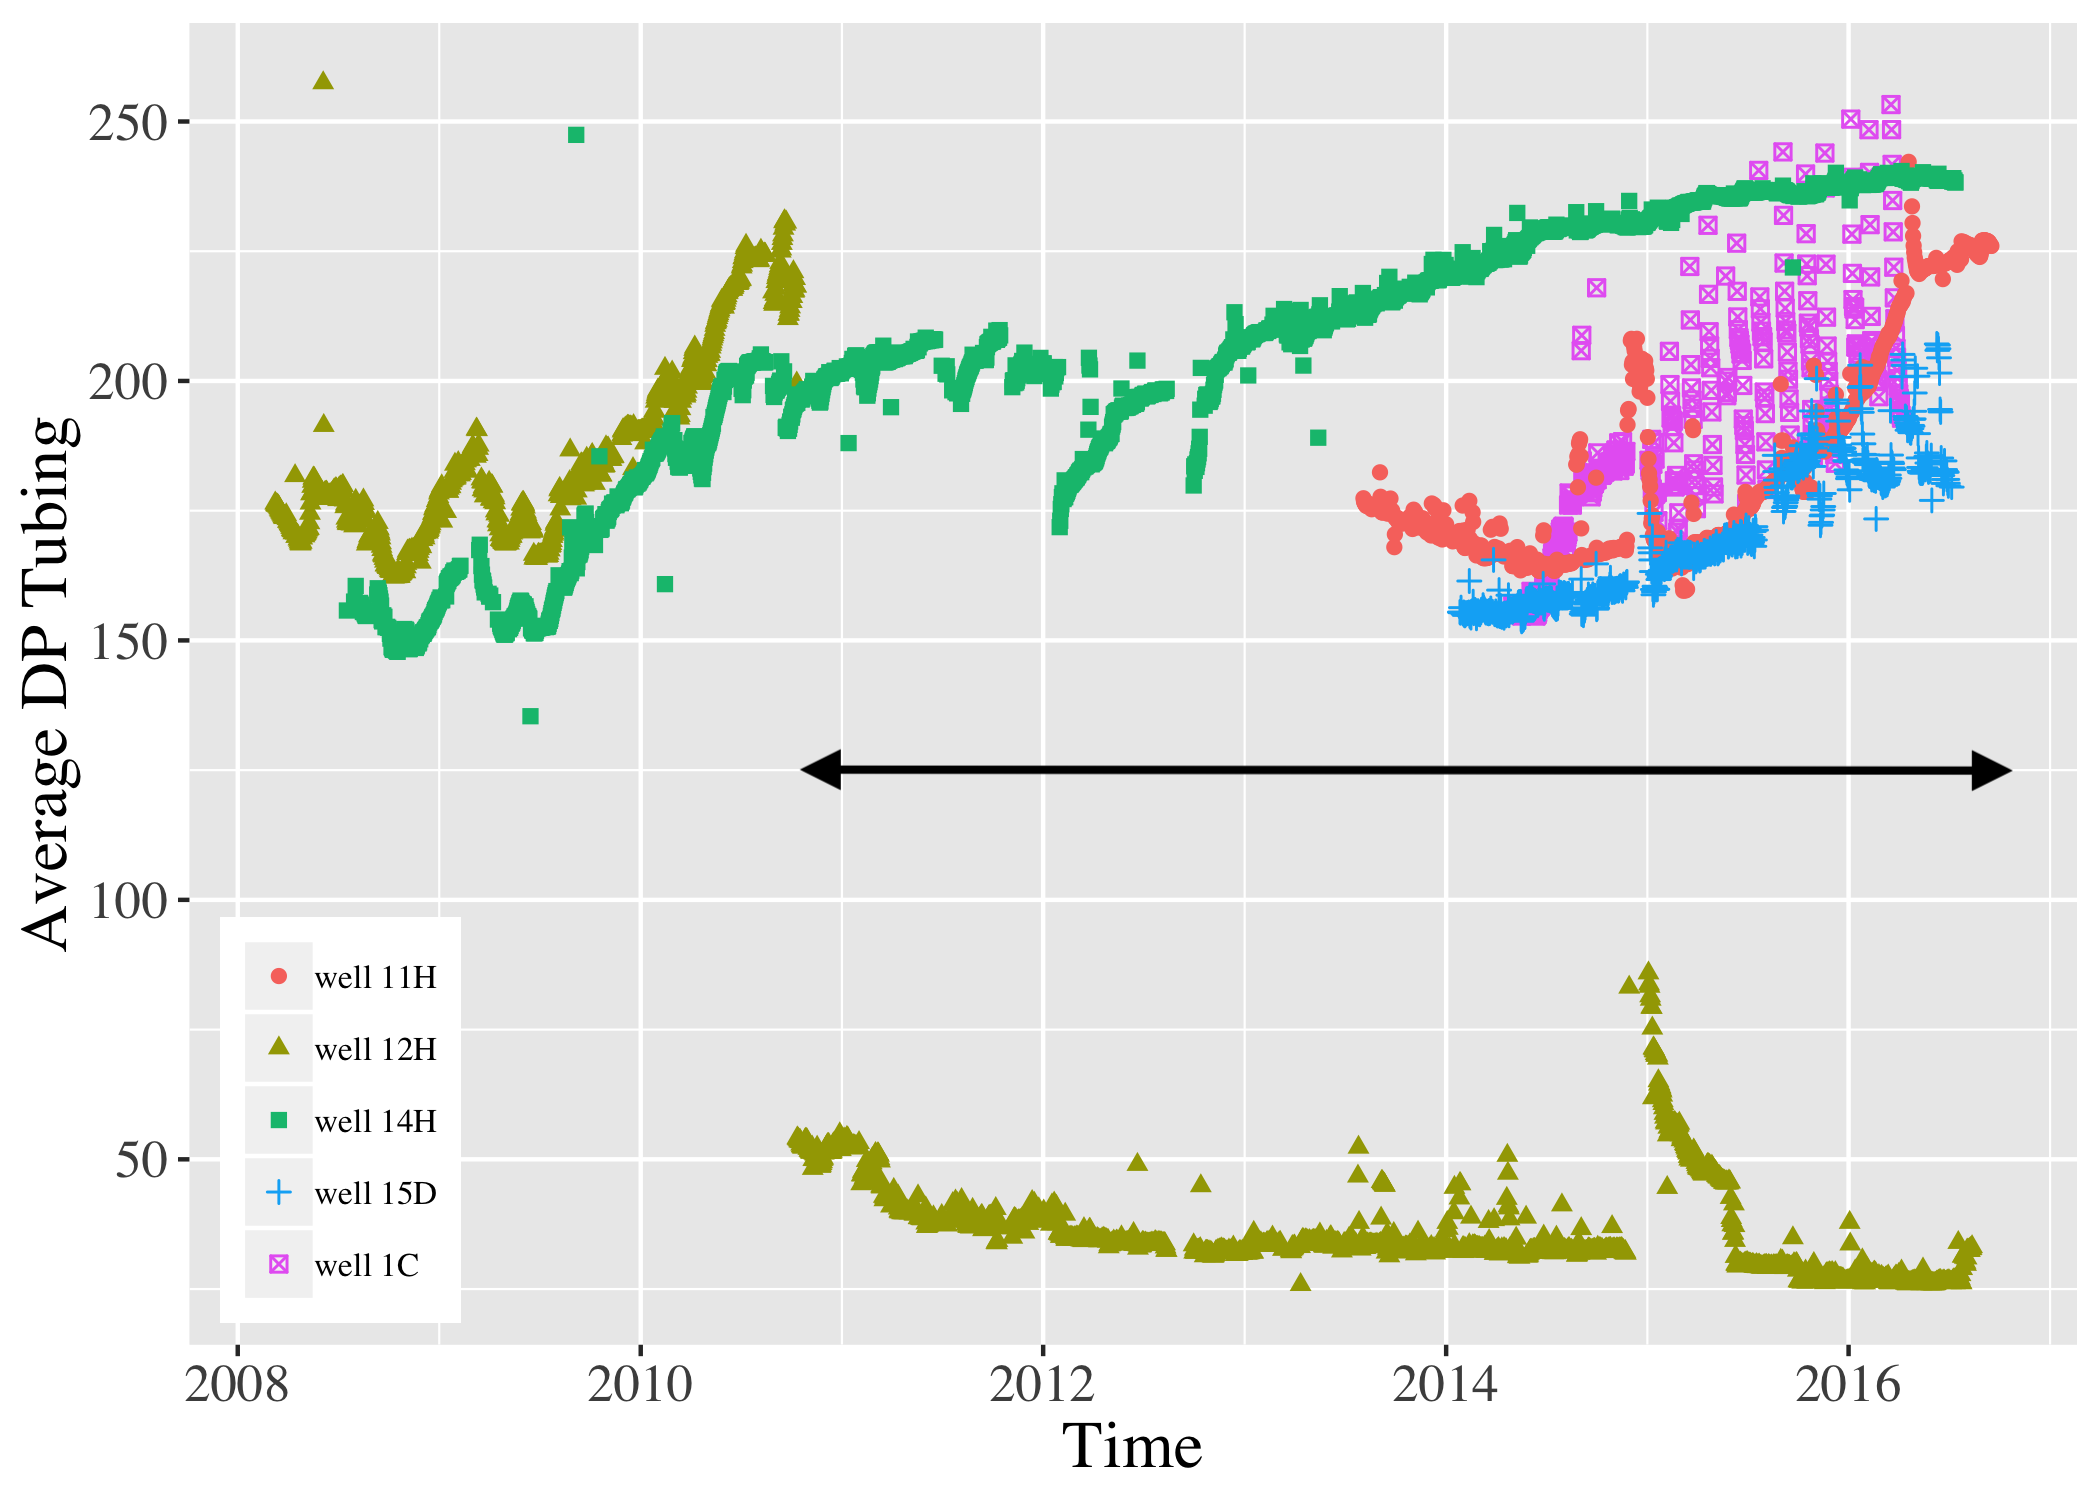
\includegraphics[width=1\linewidth,left]{adpt_t.png} 
\end{figure}

\column{.5\textwidth} % Right column and width
\begin{figure}
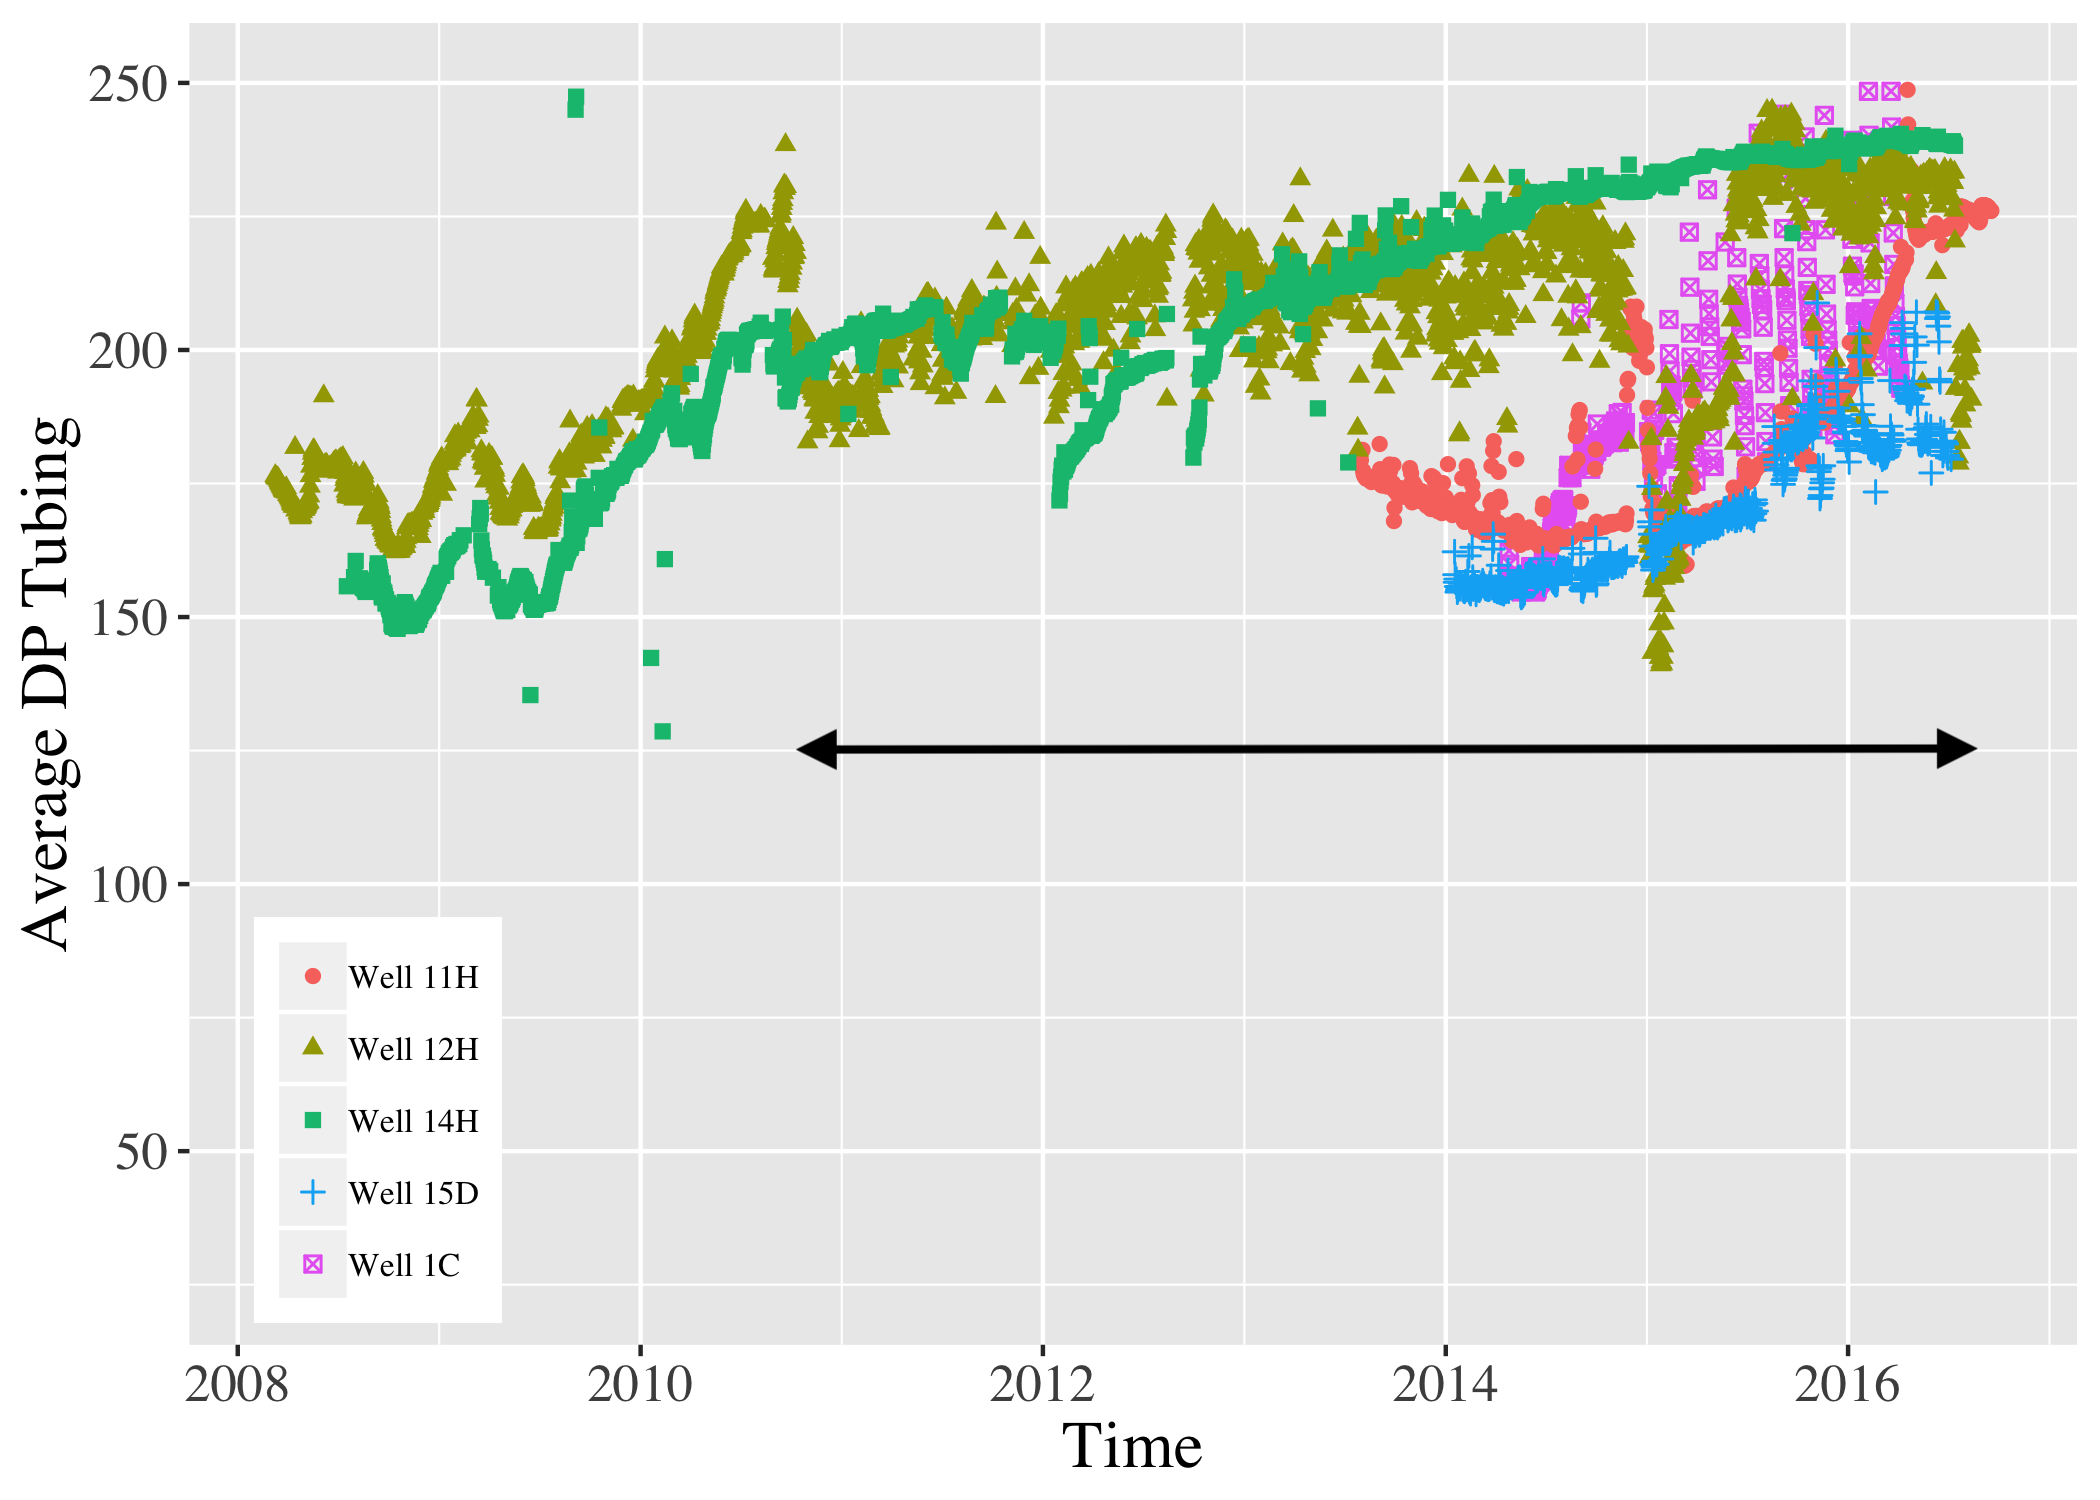
\includegraphics[width=1\linewidth, right]{pre_adpt_t.png}
\end{figure}
\end{columns}

\end{frame}


\begin{frame}
\frametitle{Data Cleansing - Missing Data Imputation}
\begin{block}{}
Some visual inspections on features before and after missing data imputation
\end{block}

\begin{columns}[c]
\column{.5\textwidth} % Left column and width
\begin{figure}
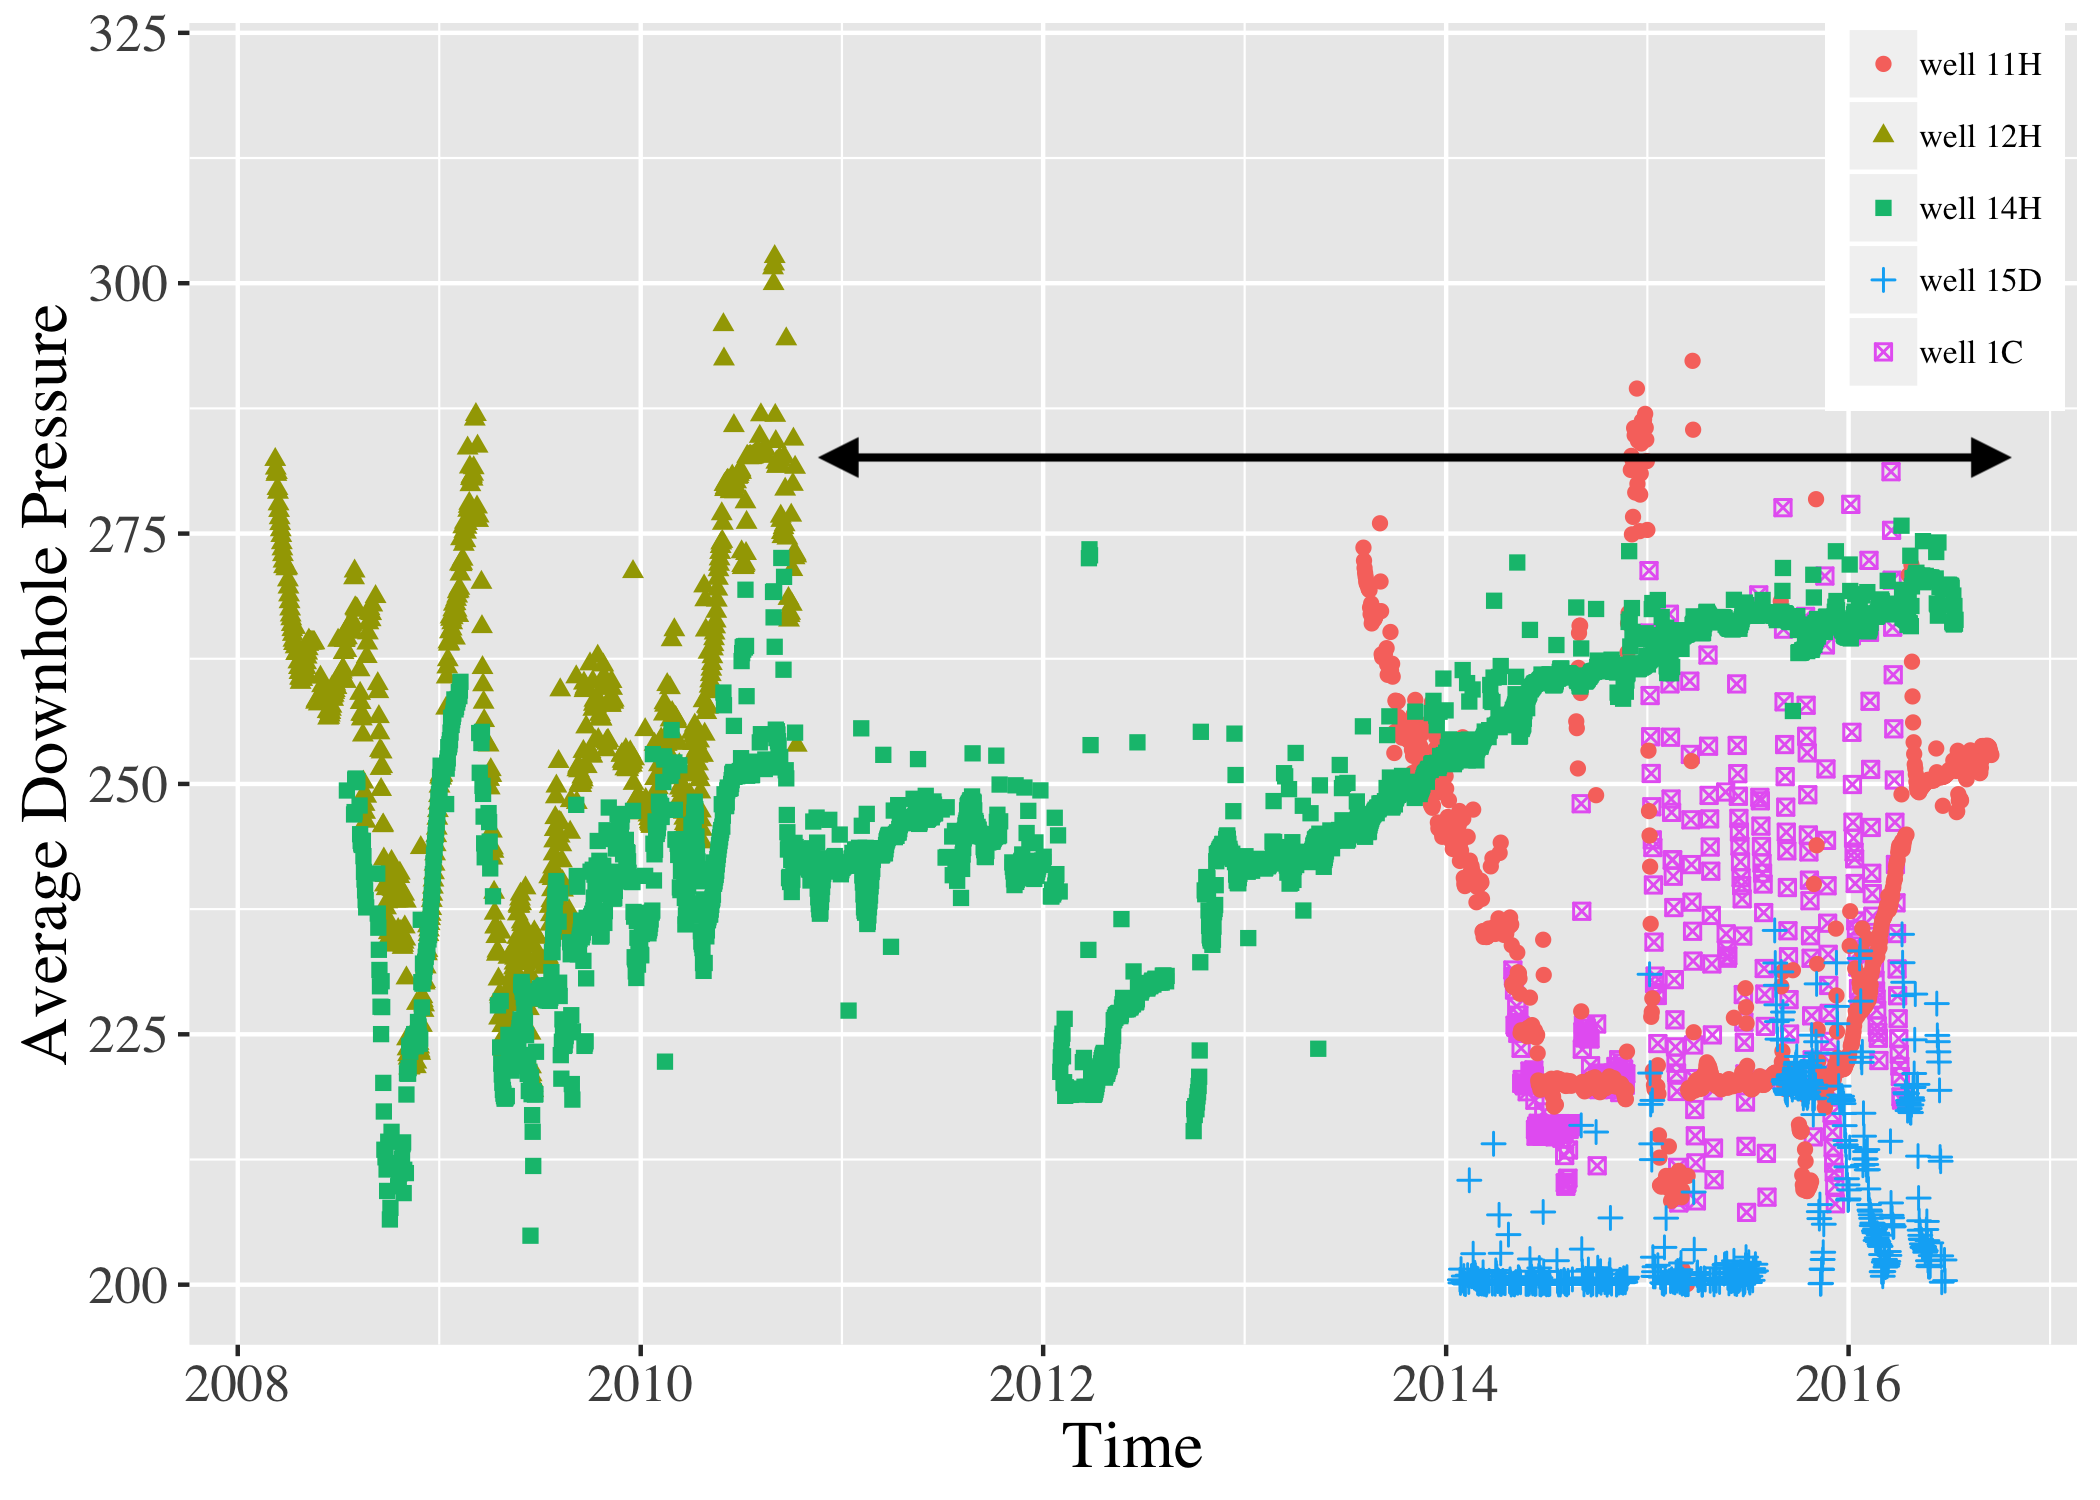
\includegraphics[width=1\linewidth,left]{adp_t_copy.png} 
\end{figure}

\column{.5\textwidth} % Right column and width
\begin{figure}
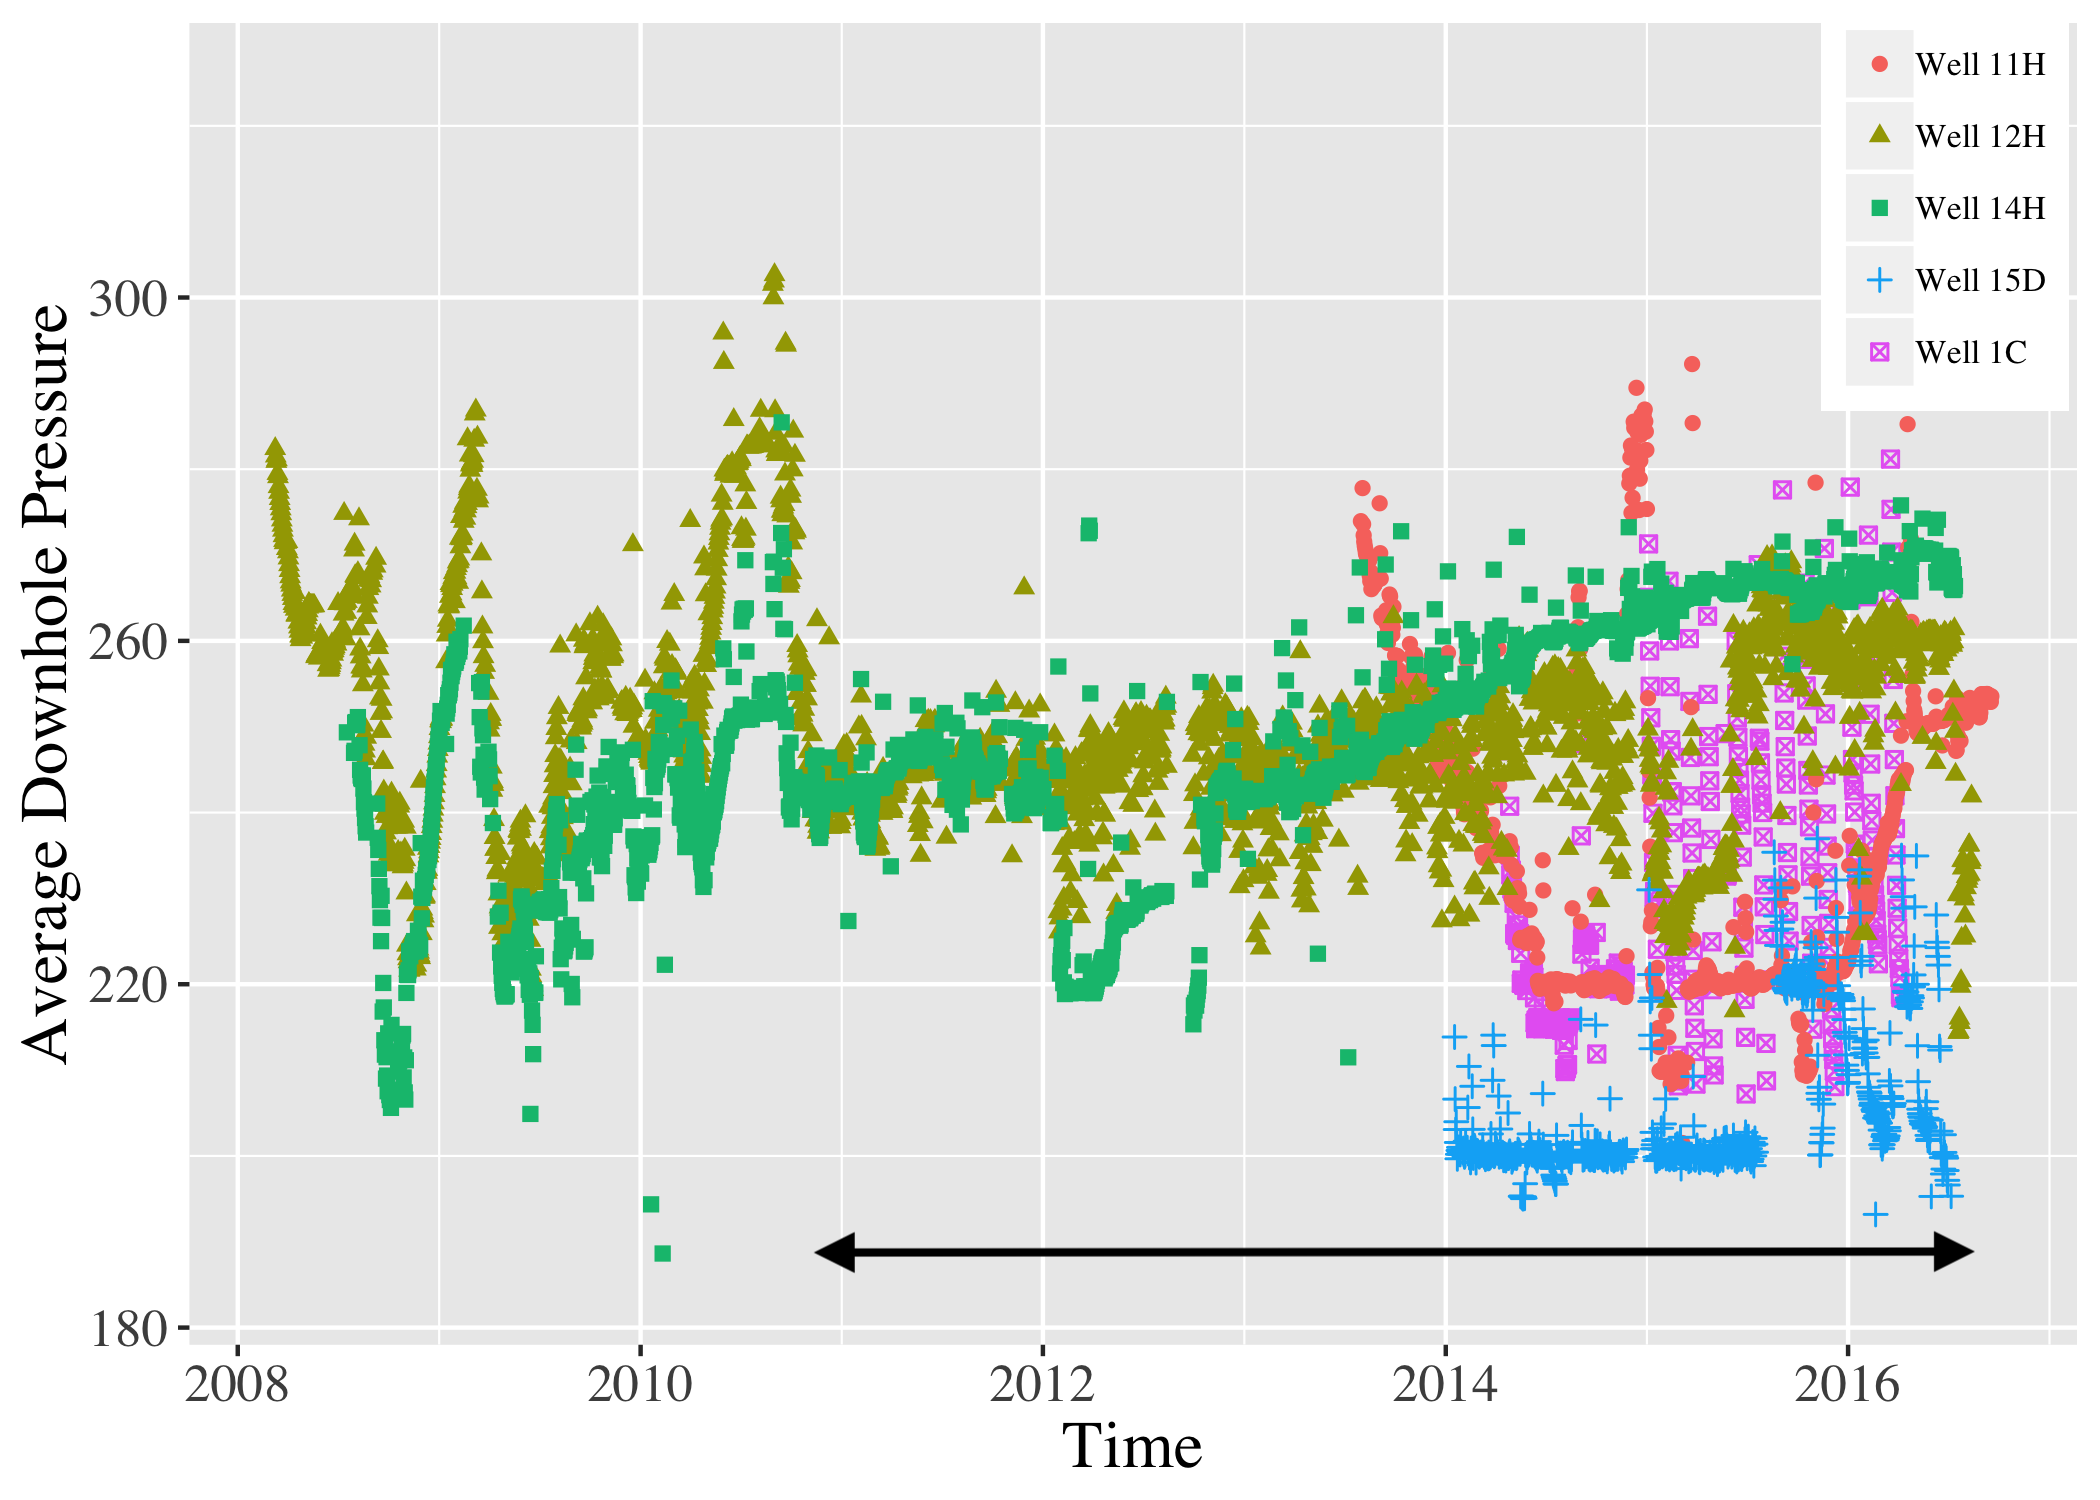
\includegraphics[width=1\linewidth, right]{pre_adp_t.png}
\end{figure}
\end{columns}

\end{frame}



\begin{frame}
\frametitle{Data Cleansing - Missing Data Imputation}
\begin{block}{}
Some visual inspections on features before and after missing data imputation
\end{block}

\begin{columns}[c]
\column{.5\textwidth} % Left column and width
\begin{figure}
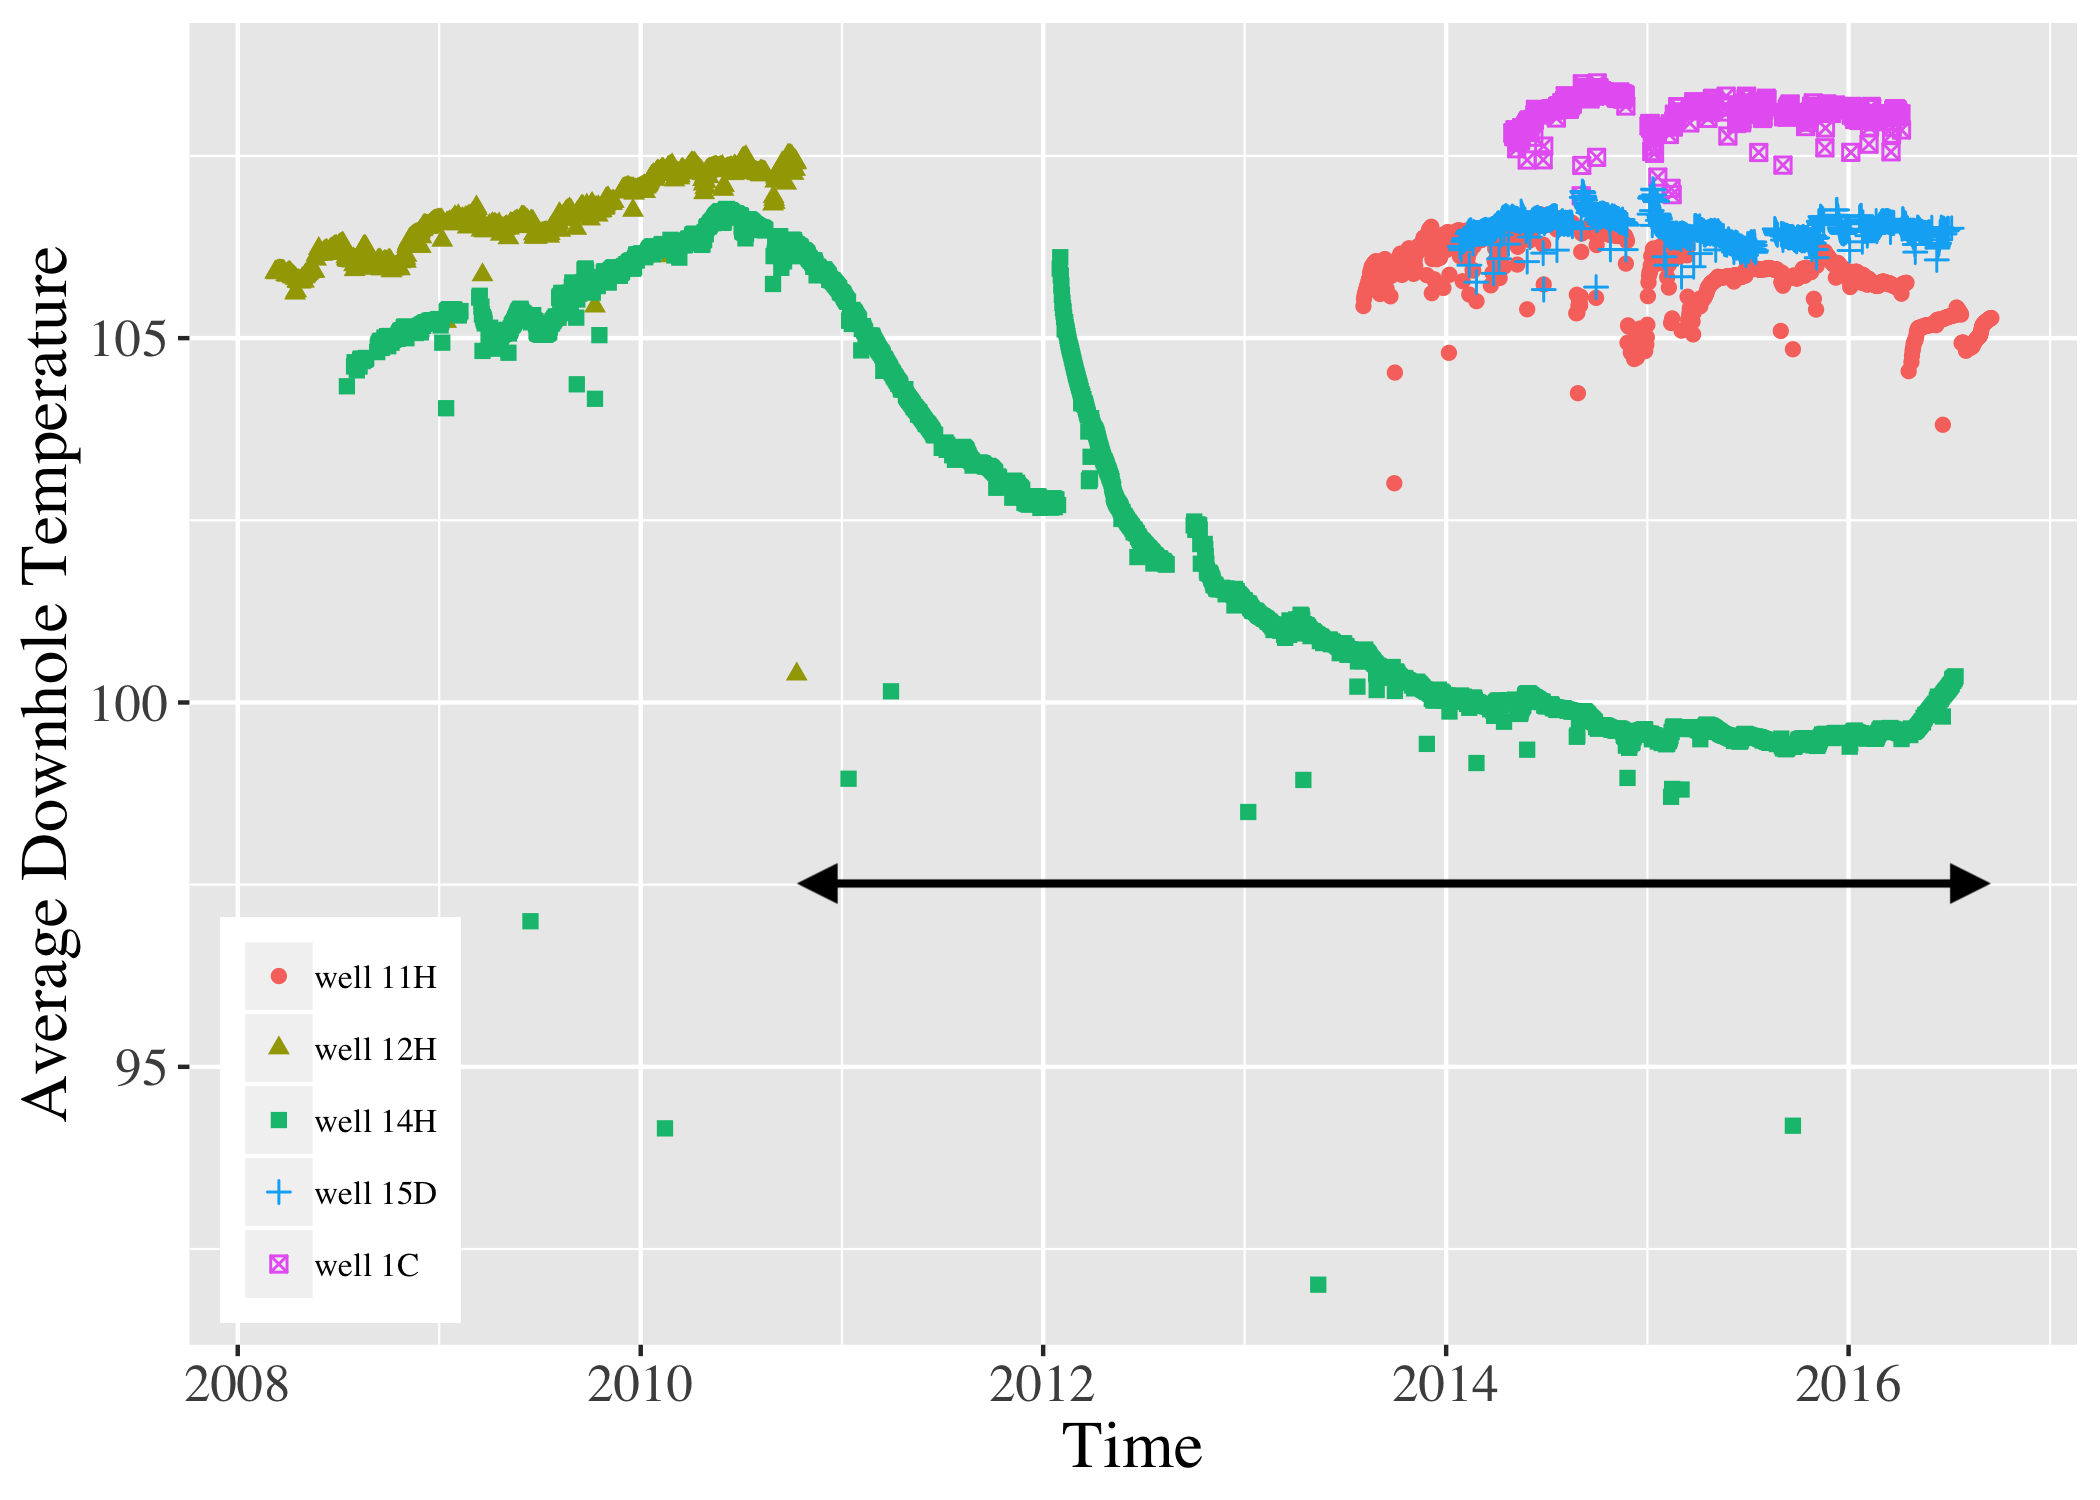
\includegraphics[width=1\linewidth,left]{adt_t_copy.png} 
\end{figure}

\column{.5\textwidth} % Right column and width
\begin{figure}
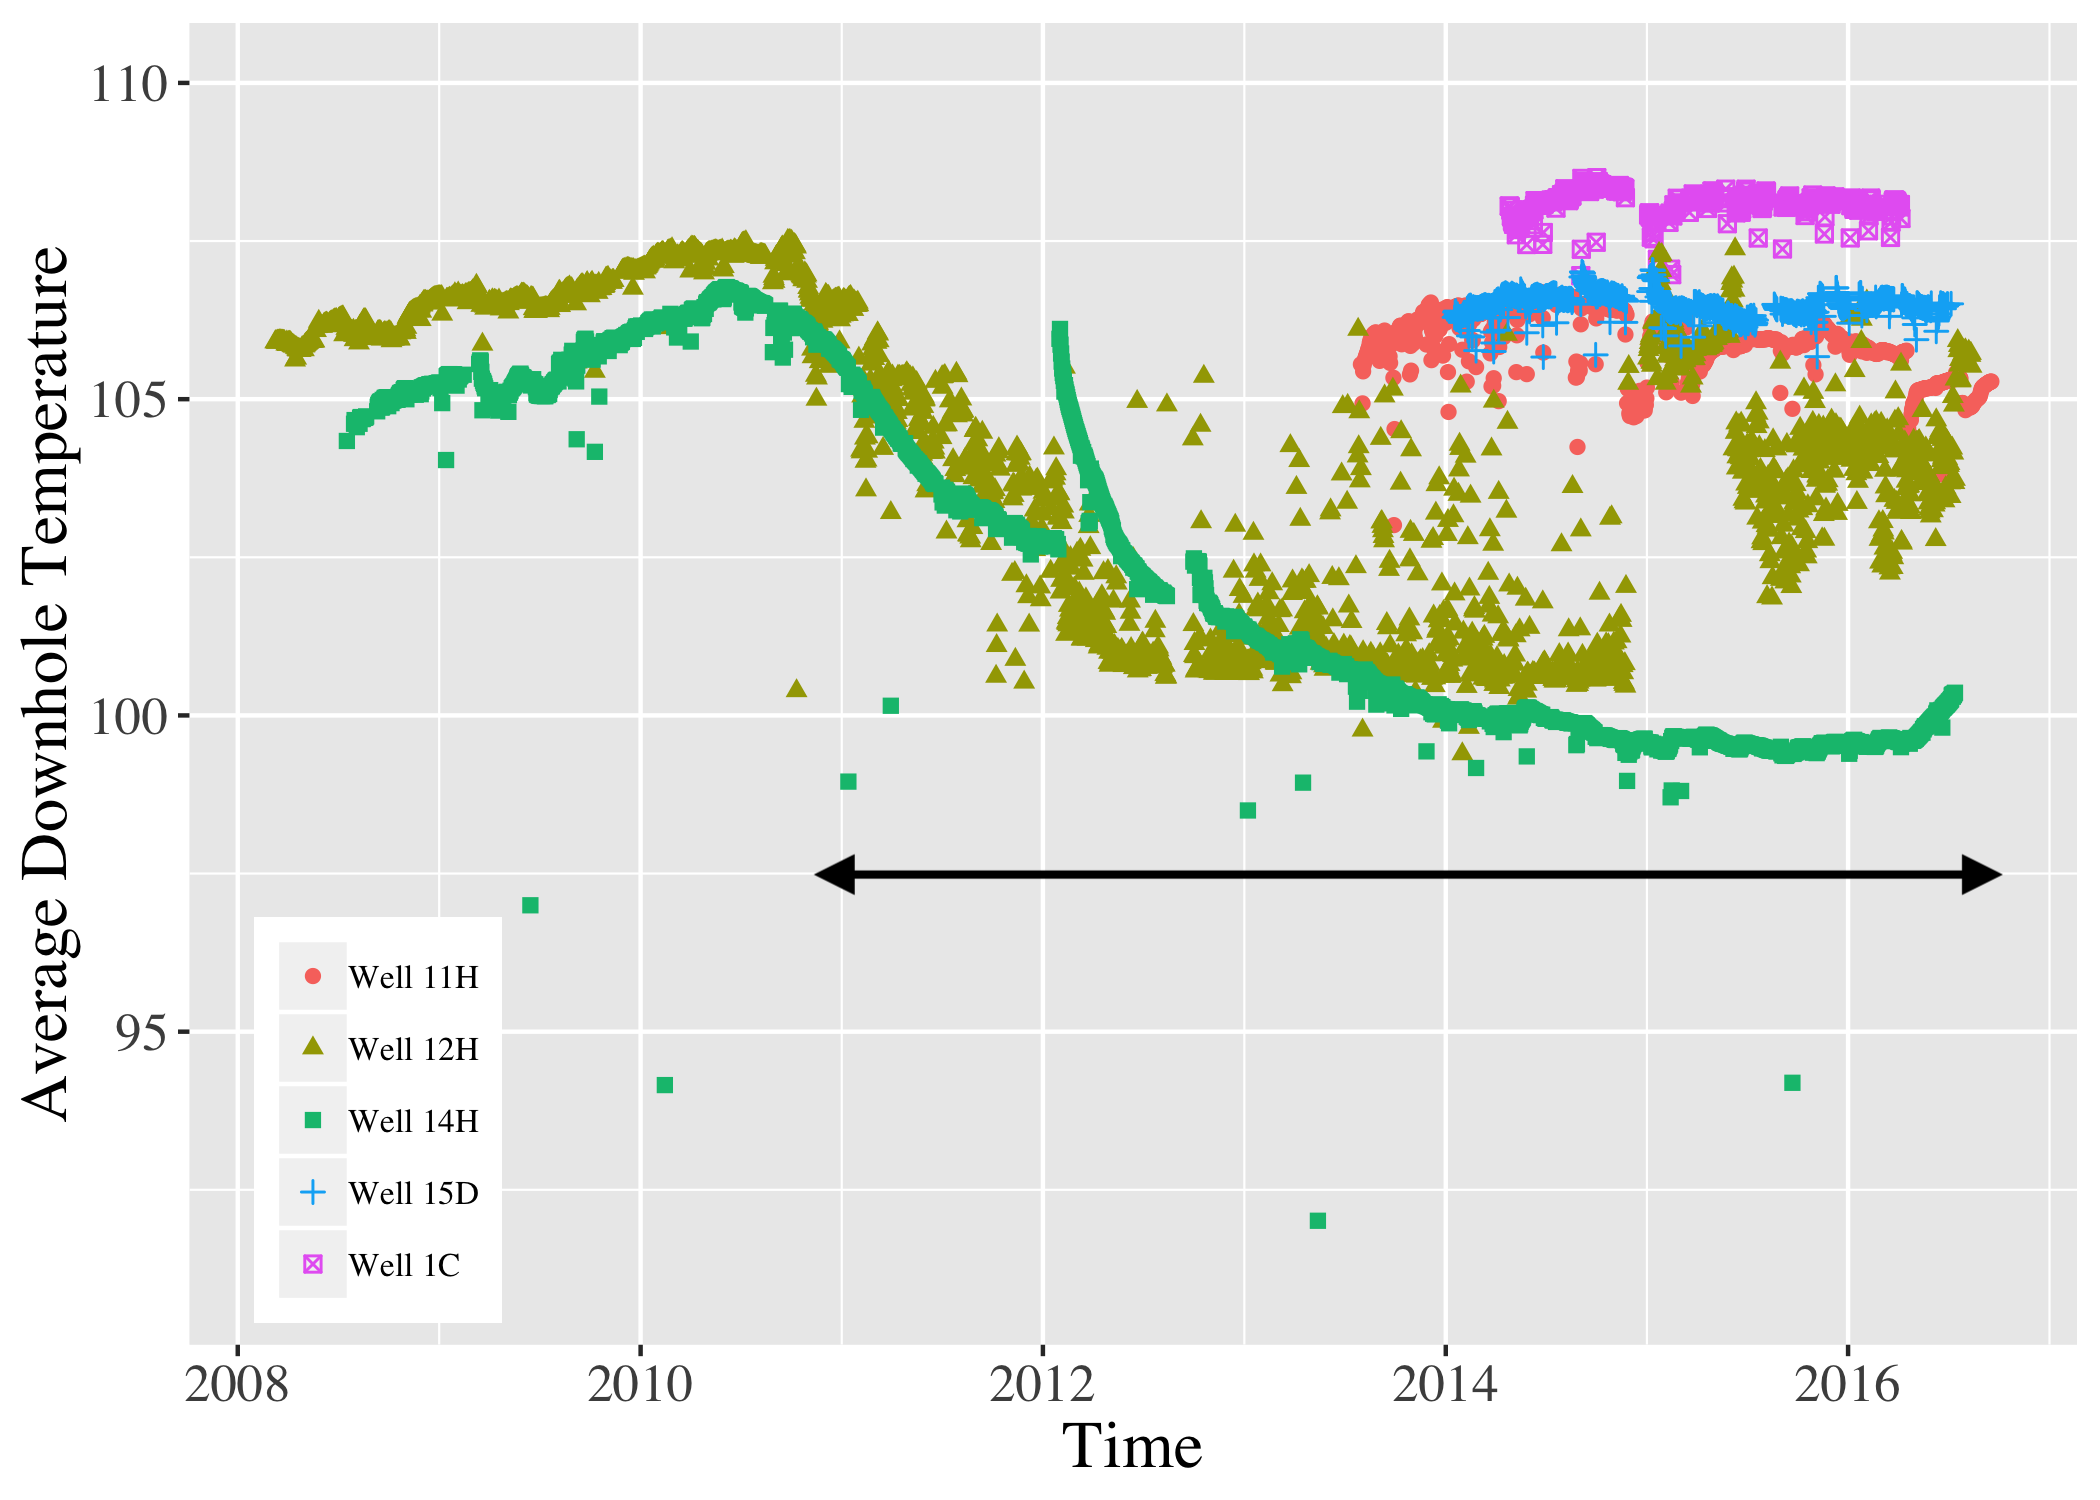
\includegraphics[width=1\linewidth, right]{pre_adt_t.png}
\end{figure}
\end{columns}

\end{frame}



\begin{frame}
\frametitle{Data Cleansing - Missing Data Imputation}
\begin{block}{}
Some visual inspections on features before and after missing data imputation
\end{block}

\begin{columns}[c]
\column{.5\textwidth} % Left column and width
\begin{figure}
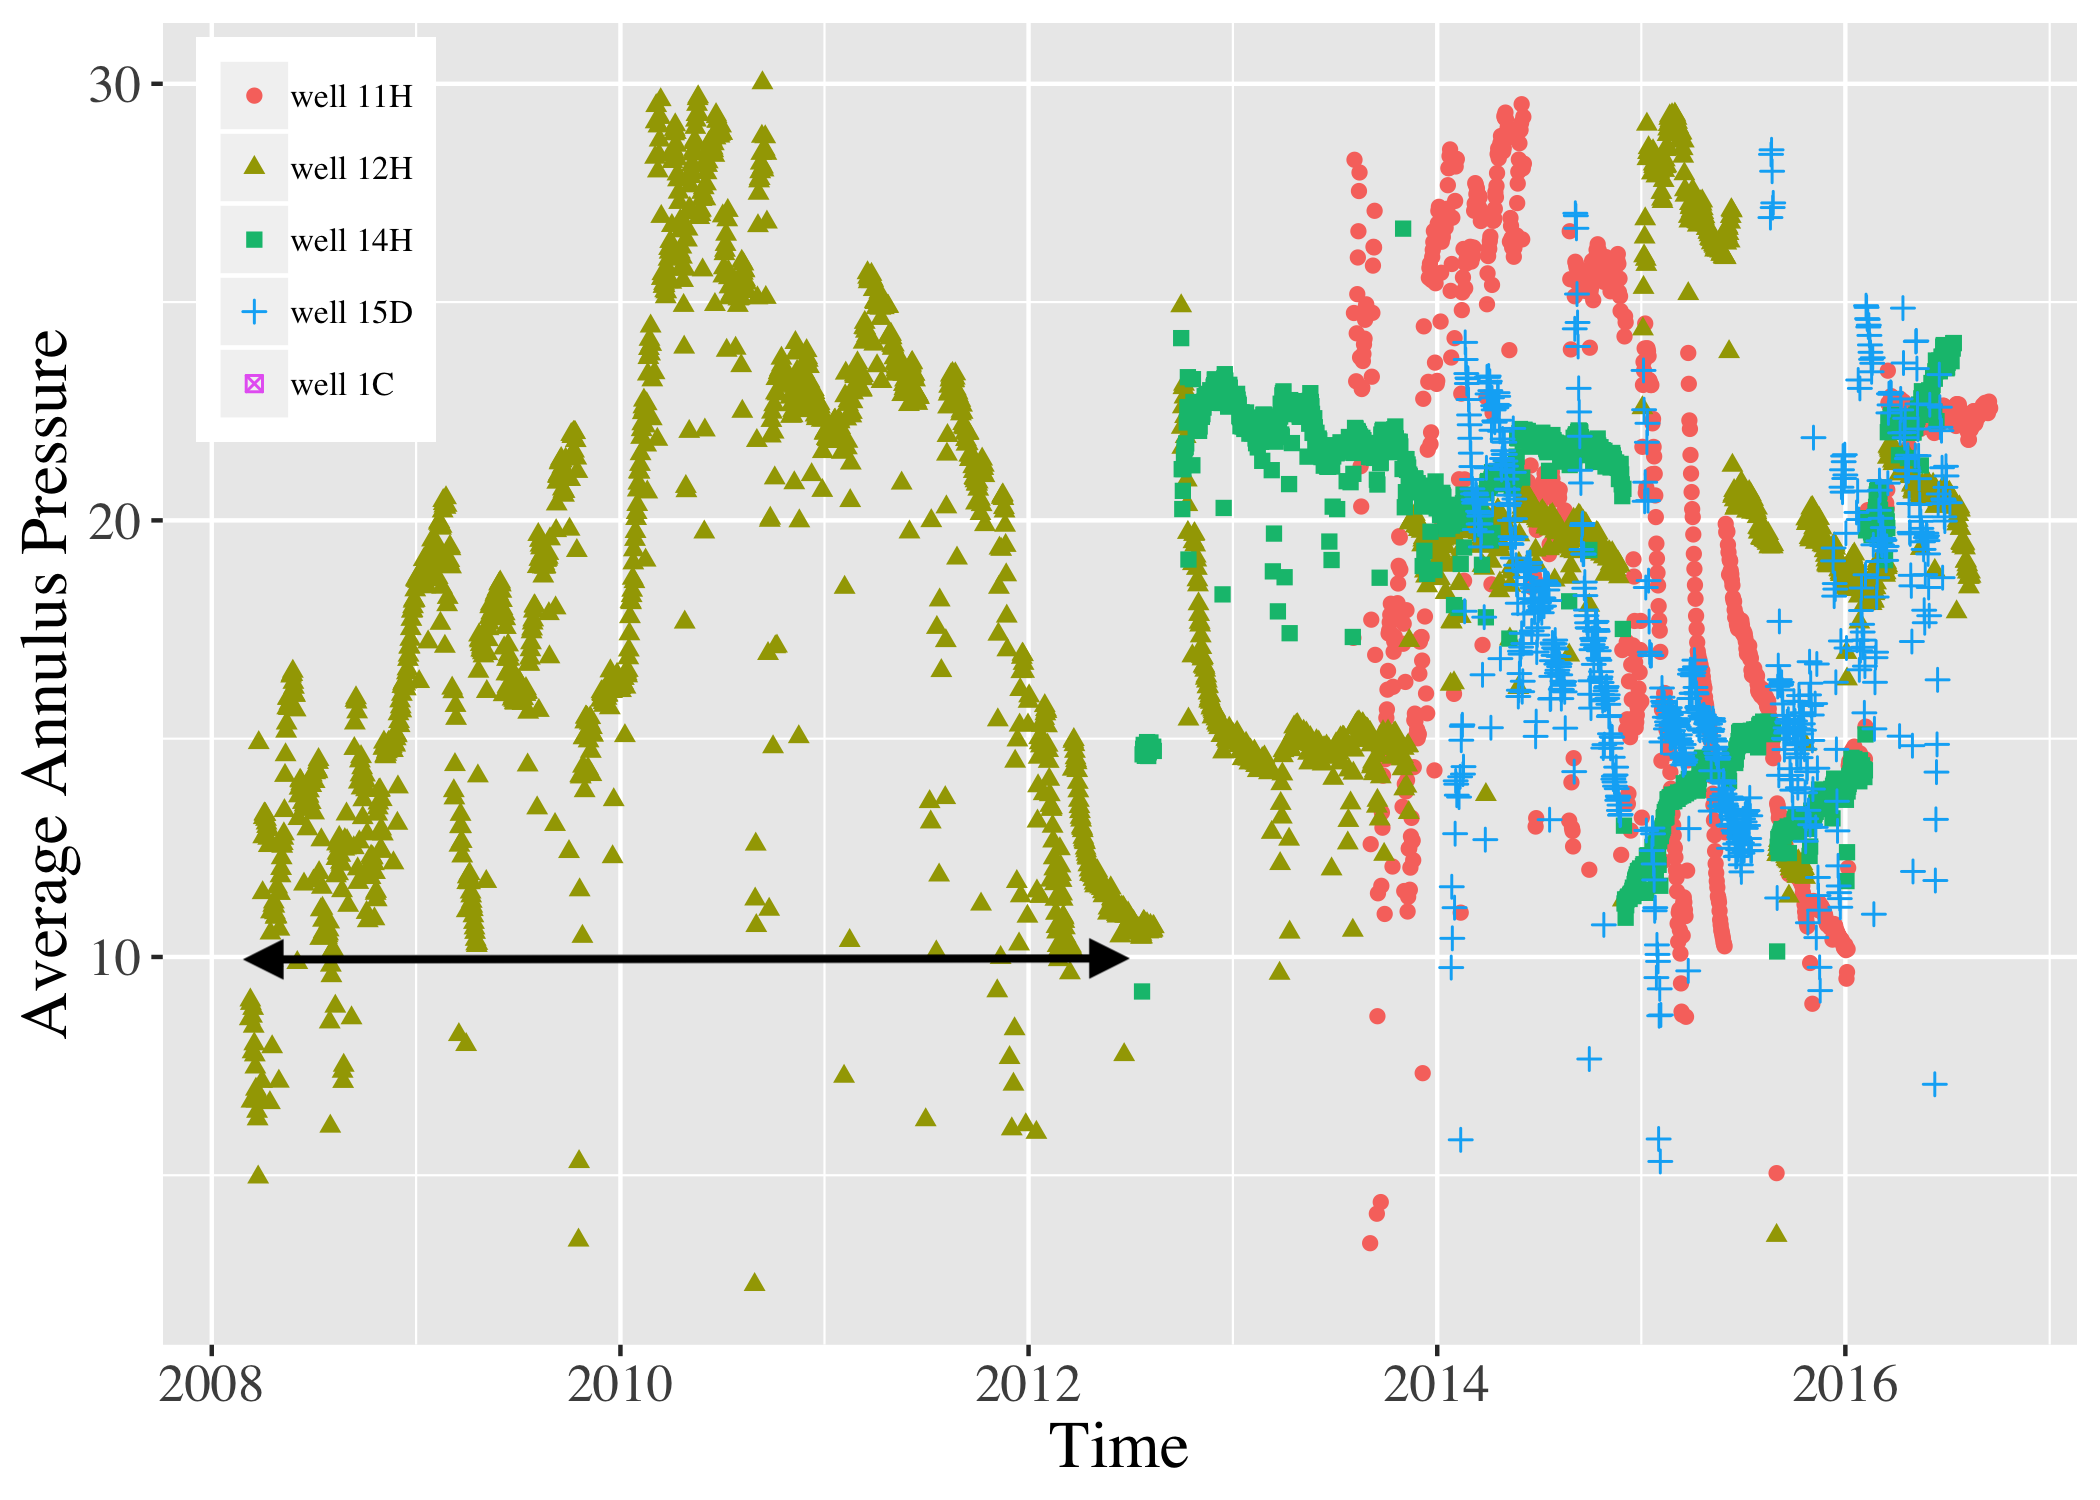
\includegraphics[width=1\linewidth,left]{aap_t_copy.png} 
\end{figure}

\column{.5\textwidth} % Right column and width
\begin{figure}
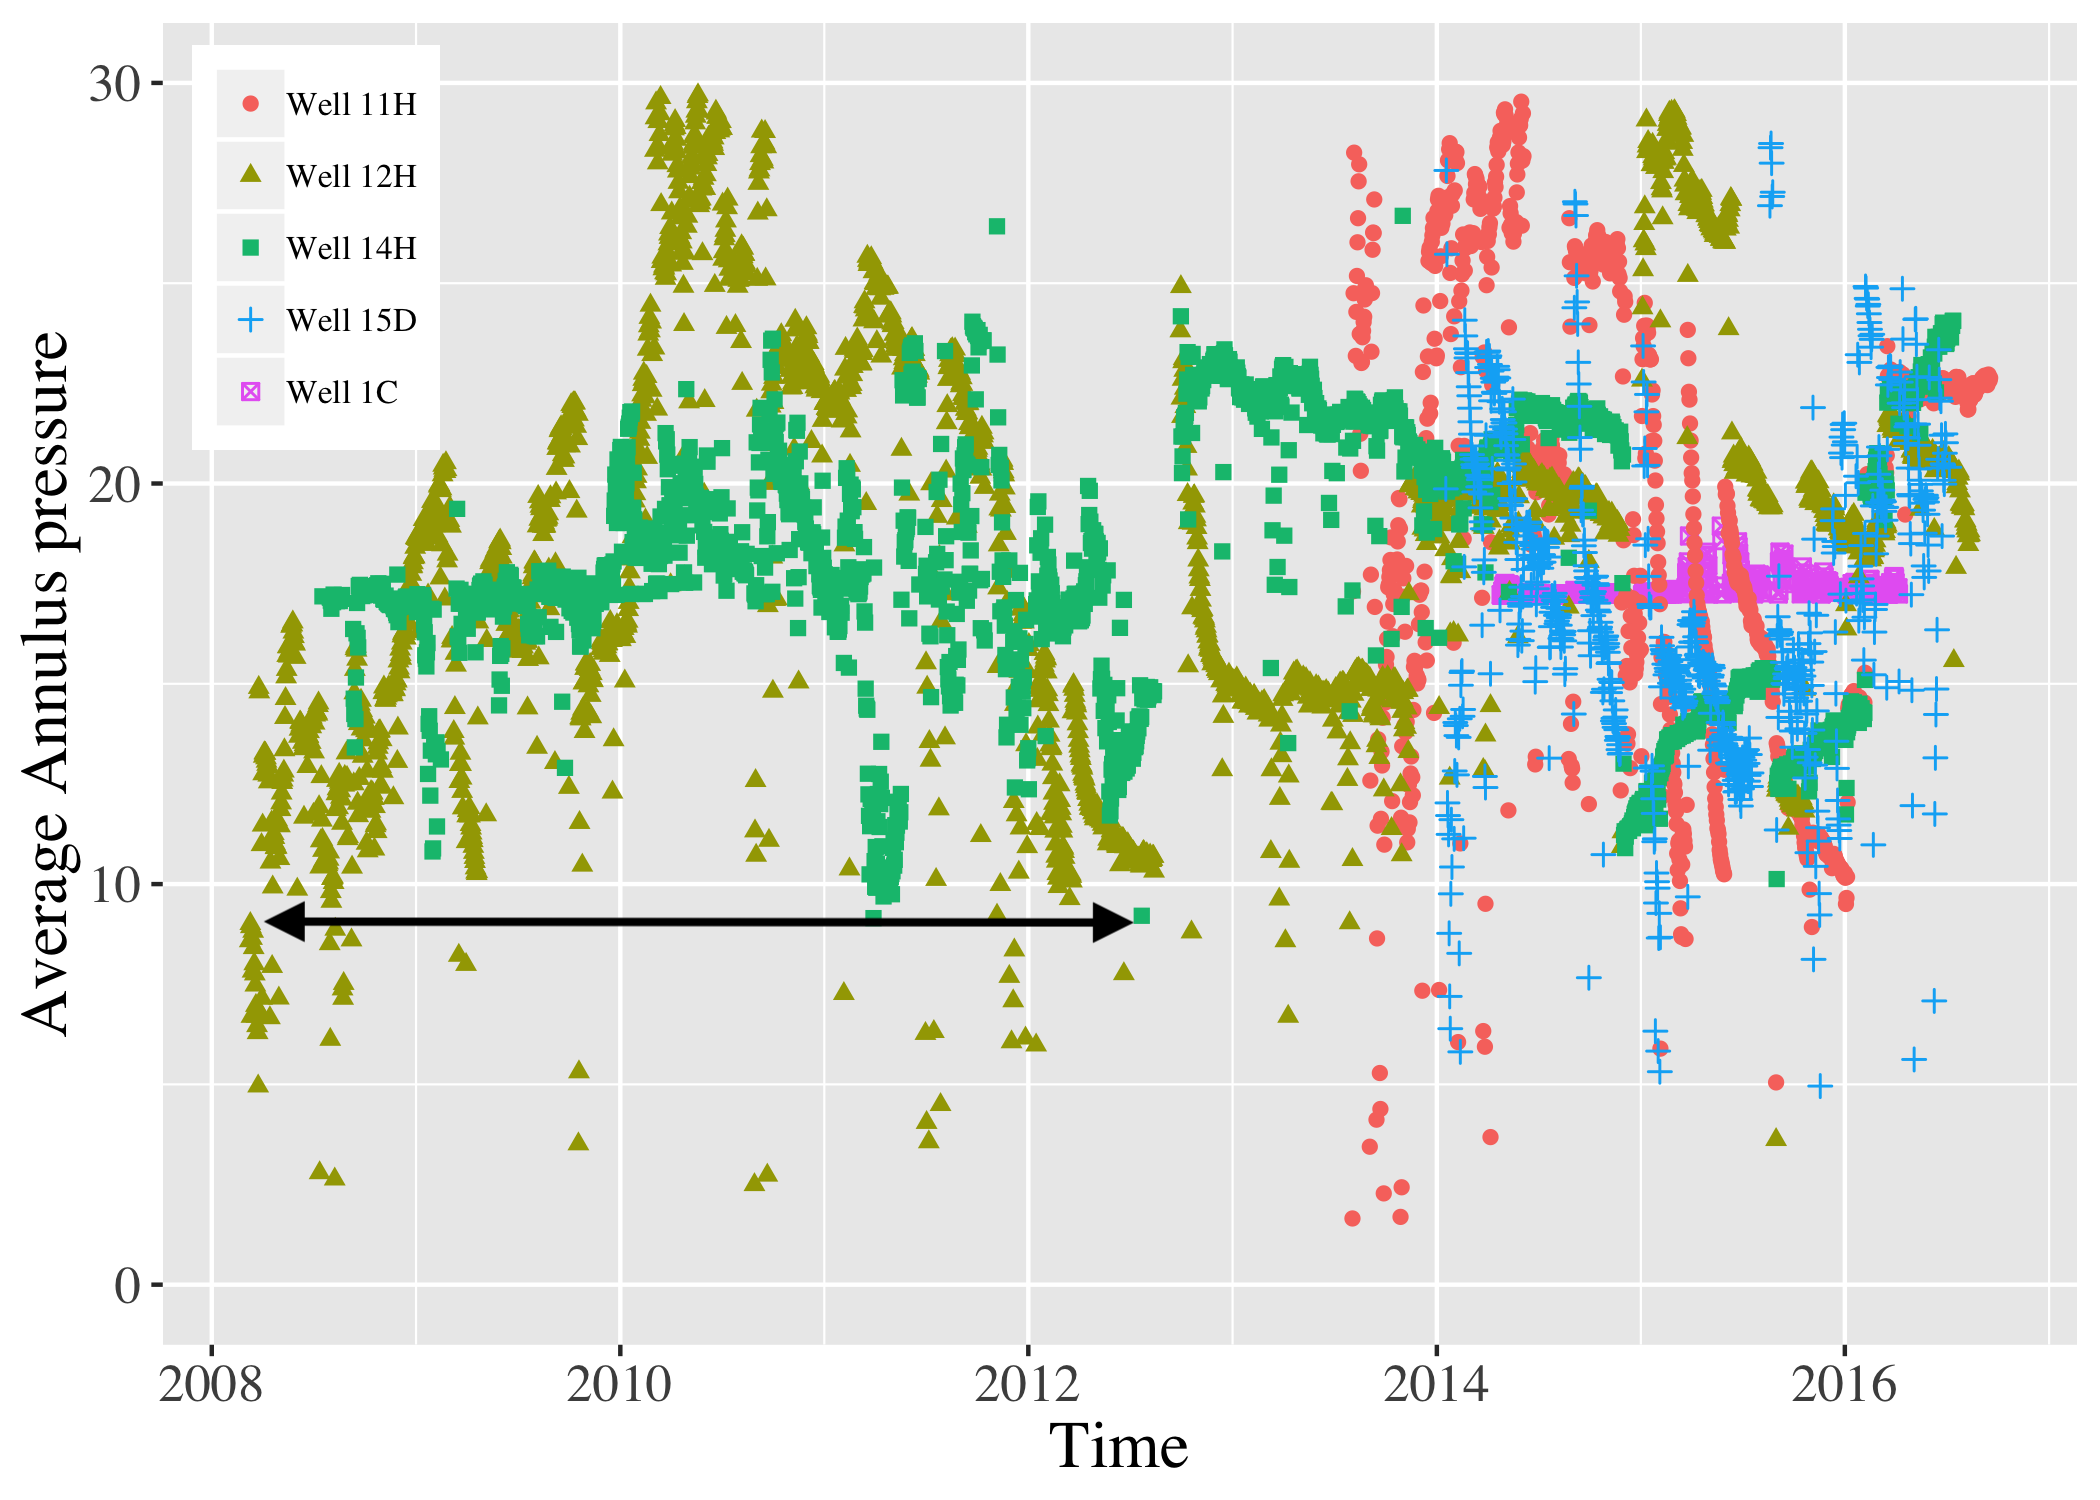
\includegraphics[width=1\linewidth, right]{pre_aap_t.png}
\end{figure}
\end{columns}

\end{frame}
%------------------------------------------------
\section{Correlation and PCA}
%------------------------------------------------

\begin{frame}
\frametitle{Data Cleansing - PCA and Correlation}


\begin{columns}[c]

\column{.6\textwidth} % Left column and width
\begin{figure}
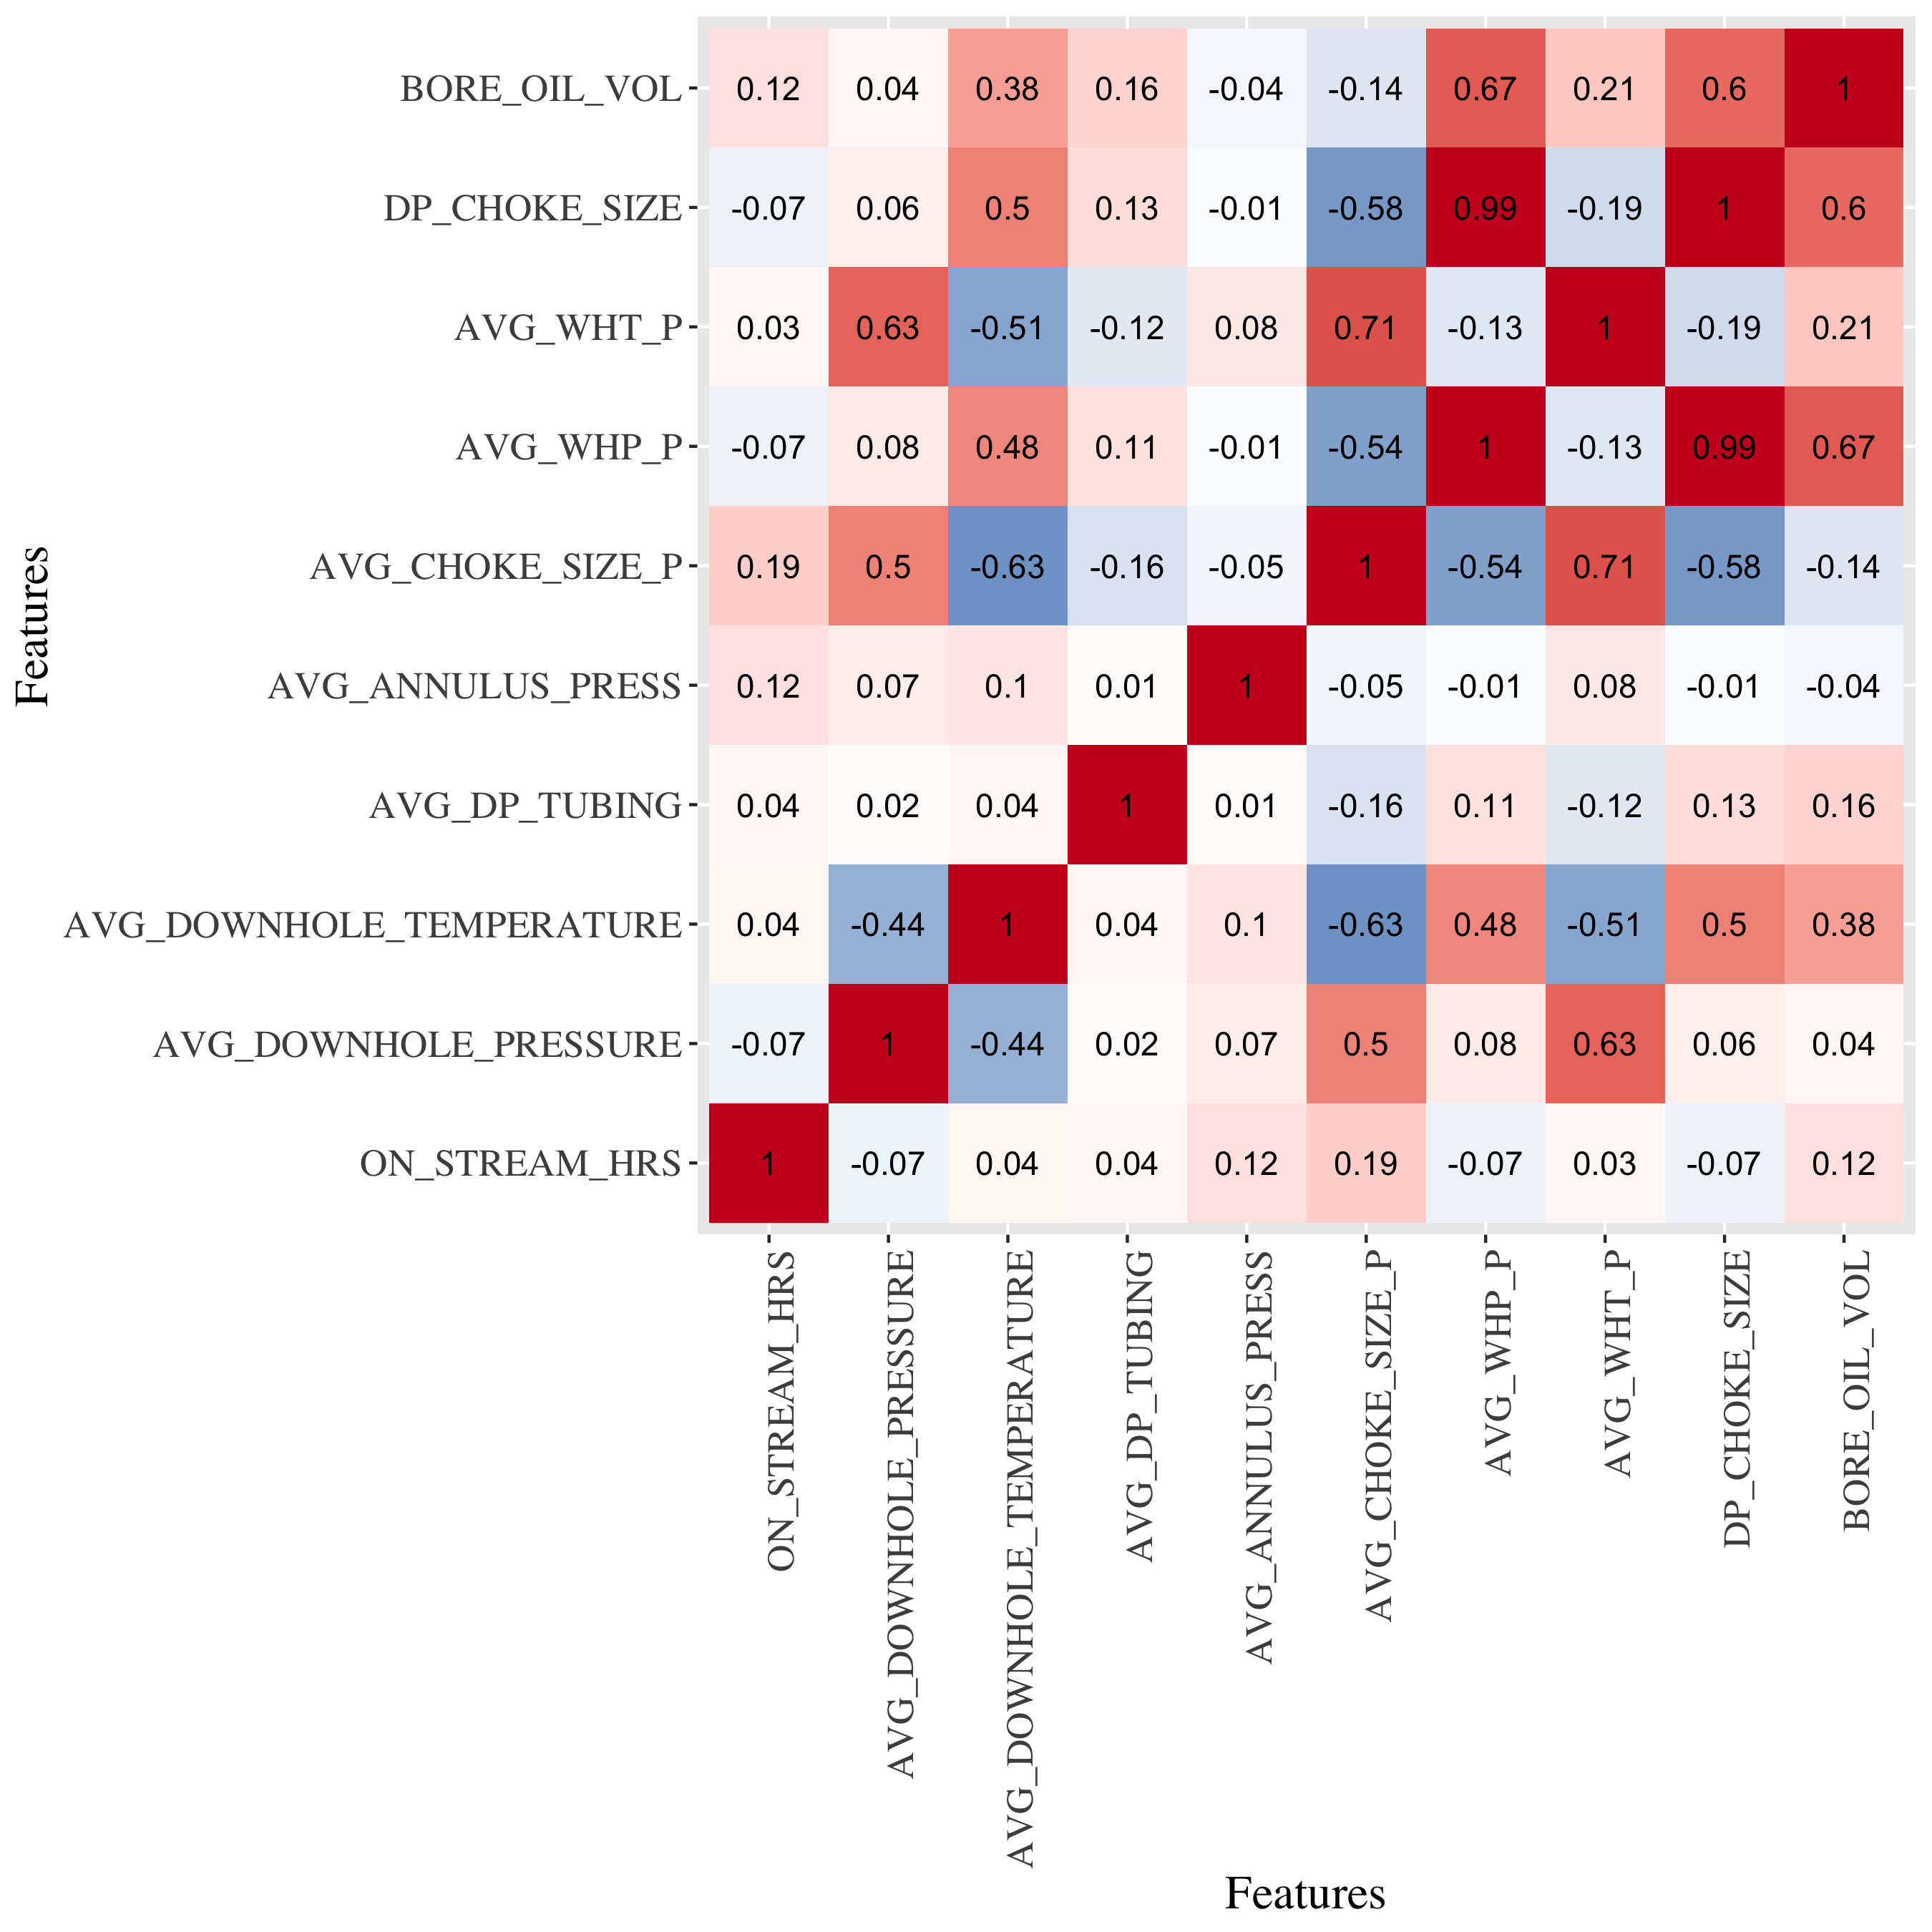
\includegraphics[width=1\linewidth,left]{corr_all.png} 
\end{figure}

\column{.4\textwidth} % Right column and width
\begin{figure}
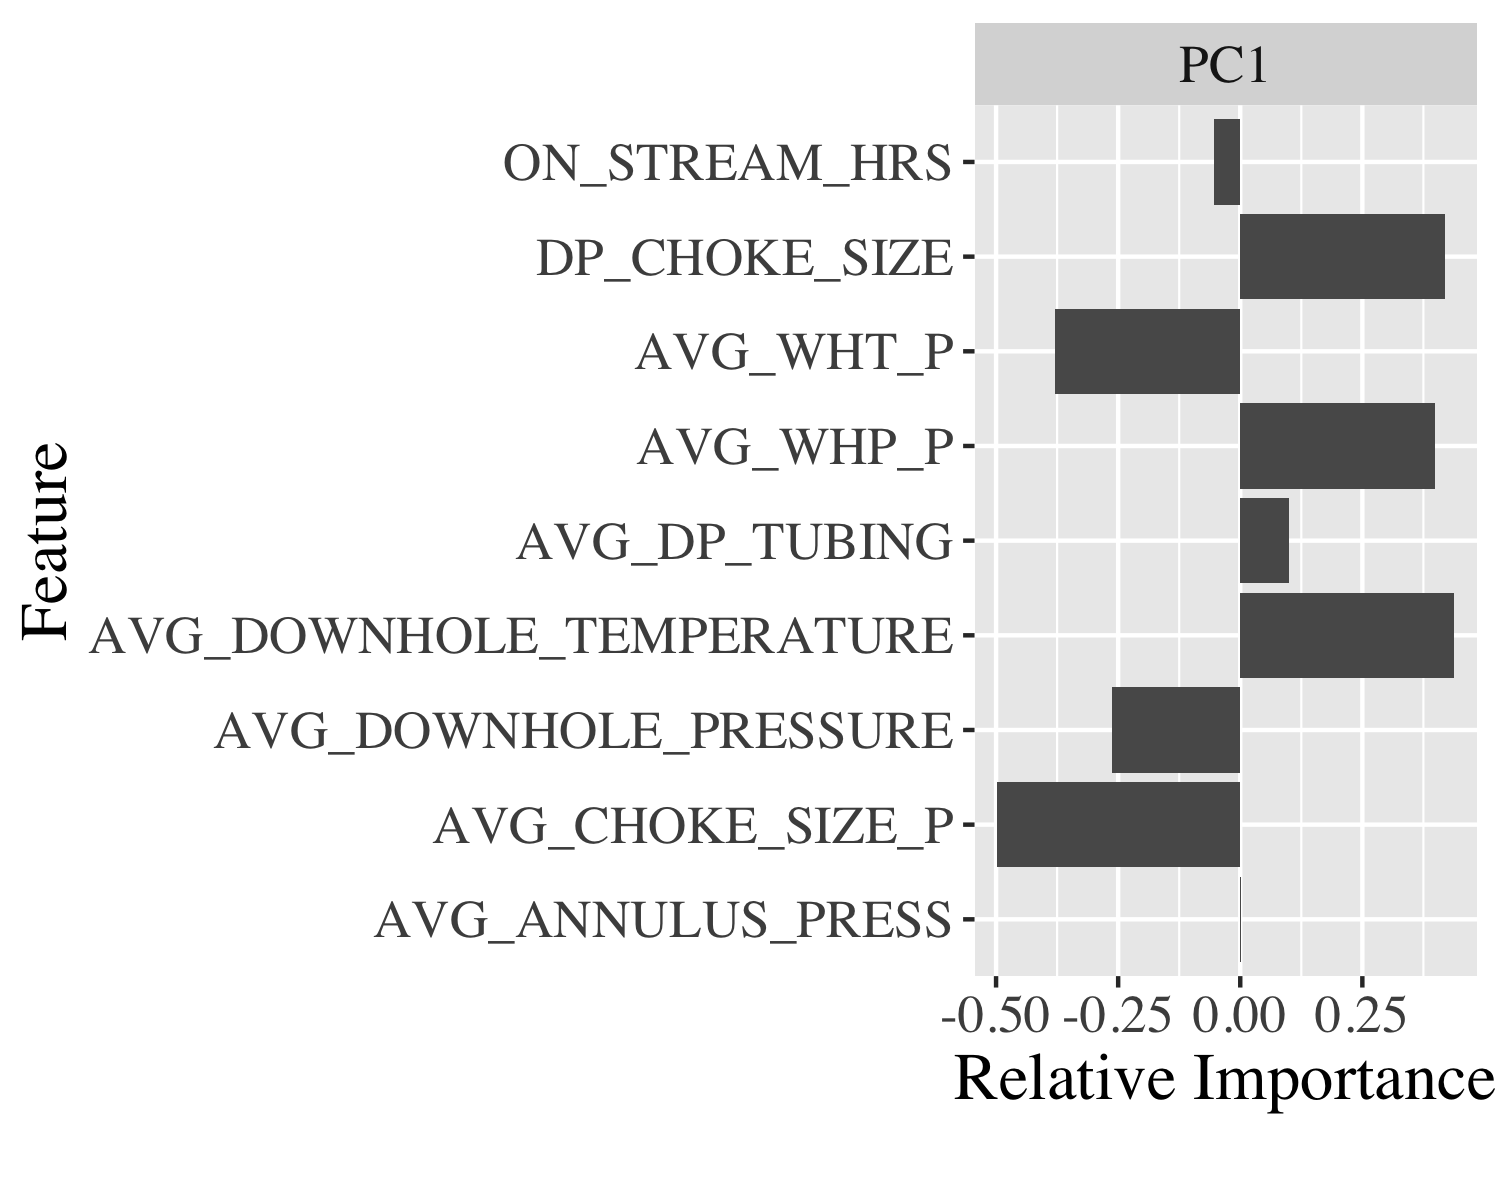
\includegraphics[width=1\linewidth, right]{pca_all.png}
\end{figure}
\end{columns}

\end{frame}




%------------------------------------------------
\section{Results}
%------------------------------------------------
\begin{frame}
\frametitle{Preliminary Results}
\begin{itemize}
\item Using cleaned data
\item Using all the features except water injection values
\item Without considering history as a feature 
\end{itemize}

\begin{table}
\begin{adjustbox}{width=1\linewidth,center}
\label{tb:rs_adpt}
\begin{tabular}{lccccccc}
\toprule
\textbf{Target}&\textbf{Model}&\textbf{R-squared}&\textbf{RMSE}&\textbf{Sigma}&\textbf{Cost}&\textbf{Layer \& Neurons}&\textbf{Epochs}\tabularnewline
\midrule
Oil production & SVR &0.97 & 2.30 & 1 & 16 & ---&--- \tabularnewline
Oil production & MLP &\cellcolor{green!40}0.98  & 0.15 & --- & --- & [32, 16] & 150 \tabularnewline

\bottomrule
\end{tabular}
\end{adjustbox}
\end{table}

\end{frame}


\begin{frame}
\frametitle{Results}
\begin{itemize}
\item Using cleaned data
\item Using all the features as well as water injection values
\item Considering history as a feature and constructing time-series data 
\item Two approaches for normalizing the datasets
\item Testing the models on different combinations of datasets
\end{itemize}


\end{frame}




\begin{frame}
\frametitle{Results - normalization approaches}

\begin{block}{Approach 1 for normalization process}
\textbf{Normalization based on the data from all wells}
\begin{itemize}
\item Setting the random seed equal to 7
\item Constructing the time series data
\item Calculating mean and standard deviation of the data
\item Normalizing the data based on mean and standard deviation
\item Shuffle the time series data
\item Splitting first 80\% data as the training set and the rest 20\% data as the test set
\end{itemize}

\end{block}

\end{frame}


\begin{frame}
\frametitle{Results - normalization approaches}

\begin{block}{Approach 2 for normalization process}
\textbf{Normalization based on the data of each well}
\begin{itemize}
\item Setting the random seed equal to 7
\item \textbf{procedure} Recursion$(Well\;Code)$
\item \hspace{5mm} Constructing the time series data
\item \hspace{5mm} Calculating mean and standard deviation of the data
\item \hspace{5mm} Normalizing the data based on mean and standard deviation
\item \hspace{5mm} Shuffle the time series data
\item \hspace{5mm} Splitting first 80\% data as the training and the rest 20\% as the test set
\item  \textbf{end procedure} 
\item Concatenating the training set and the test set
\end{itemize}

\end{block}

\end{frame}


\begin{frame}
\frametitle{Results -SVR}

\begin{block}{Constructing time series data for SVR model}
\begin{equation}
\begin{split}
	X_{SVR} = [Var_1(t-n), Var_2(t-n), \cdots, Var_m(t-n), label(t-n), \cdots, 
	\\Var_1(t-1), Var_2(t-1), \cdots, Var_m(t-1), label(t-1), 
	\\ \cdots, Var_1(t)Var_2(t) \cdots Var_m(t)],
\end{split}
\end{equation}
where $Var_i$ is the $i$th feature, and $label(t-j)$ is the oil production value of time step $j$.
The output $Y_{SVR}$ of SVR is:
\begin{equation}
	Y_{SVR} = [label(t)].	
\end{equation}
\end{block}

\end{frame}



\begin{frame}
\frametitle{Results - SVR}
 \begin{block}{}
Average Results of time series oil production prediction using SVR\\
Grid search on different sigma and cost values\\
Training and testing the model using different time-steps; 1,3,5,10 and 20
\end{block}

 \begin{table}[H]
 \begin{adjustbox}{width=0.9\linewidth,center}
 
 		\begin{tabular}{cccccccc}
 			\toprule
 			\multicolumn{1}{c}{dataset}&\multicolumn{1}{c}{normalization}&\multicolumn{1}{c}{R-squared}&\multicolumn{1}{c}{RMSE}&\multicolumn{1}{c}{time-step}&\multicolumn{1}{c}{cost}&\multicolumn{1}{c}{sigma}\tabularnewline
 			\midrule
 			\{1C\} & Each & 0.93 & 0.25 & 5 &100 & 0.0001\tabularnewline
 			\{11H\} & Each & 0.86 & 0.34 & 5 &100 & 0.001\tabularnewline
 			\{15D\} & Each &  0.95& 0.21 & 5 &100 & 0.0005\tabularnewline
 			\{12H, 14H\}& All &\cellcolor{green!40}0.99 & 0.08 & 5 &16 & 0.001\tabularnewline
 			\{1C, 11H\} & All & 0.97 & 0.18 & 5 &64 & 0.004\tabularnewline
 			\{1C, 11H\} & Each & 0.93 & 0.25 & 5 &64 & 0.004\tabularnewline
 			\{1C, 11H, 15D\}  & All &\cellcolor{green!40} 0.98 & 0.12 & 5 &100 & 0.001\tabularnewline
 			\{1C, 11H, 15D\}  & Each & 0.92 & 0.29 & 5 &100 & 0.001\tabularnewline
 			\{12H, 14H, 1C, 11H, 15D\}  & All &\cellcolor{green!40} 0.99 & 0.08 & 5 &100 & 0.001\tabularnewline
 			\{12H, 14H, 1C, 11H, 15D\}  & Each & 0.97 & 0.18 & 5 &100 & 0.001\tabularnewline
 			\bottomrule
 	\end{tabular}
	\end{adjustbox}
 \end{table}
 
\end{frame}

\begin{frame}
\frametitle{Results - LSTM}

\begin{block}{Constructing time series data for LSTM model}
\begin{equation}
X_{LSTM} =	\Bigg[\begin{array}{c c c c}
Var_1{t-n} & Var_2{t-n} & \cdots & Var_m{t-n}\\
\vdots & \vdots & \cdots & \vdots \\
Var_1{t-1} & Var_2{t-1} & \cdots & Var_m{t-1}\\
Var_1{t} & Var_2{t}& \cdots & Var_m{t}\\
\end{array}\Bigg],
\end{equation}

and Output $Y_{LSTM}$ is:
\begin{equation}
Y_{LSTM} = [label(t)].	
\end{equation}

\end{block}

\end{frame}

\begin{frame}
\frametitle{Results - LSTM}
 \begin{block}{}
Average Results of time series oil production prediction using LSTM\\
Training and testing the model using different time-steps; 1,3,5,10 and 20\\
Best time-step: \textbf{10 days}\\
Number of neurons: 50\\
Training epochs: 100
\end{block}

 \begin{table}[H]
 \begin{adjustbox}{width=0.8\linewidth,center}
 
 		\begin{tabular}{ccccc}
 			\toprule
 			\multicolumn{1}{c}{dataset}&\multicolumn{1}{c}{normalization}&\multicolumn{1}{c}{R-squared}&\multicolumn{1}{c}{RMSE}\tabularnewline
 			\midrule
 			\{1C\}\ & Each &  0.91 & 0.26 \tabularnewline
			\{11H\} & Each &  0.96 & 0.2 \tabularnewline
			\{15D\} & Each &  0.84 & 0.36\tabularnewline
			\{12H, 14H\} & All &\cellcolor{green!40}0.99 & 0.08 \tabularnewline
			\{1C, 11H\} & All &\cellcolor{green!40} 0.98 & 0.122\tabularnewline
			\{1C, 11H\} & Each & 0.96 & 0.2\tabularnewline
			\{1C, 11H, 15D\} & All &\cellcolor{green!40} 0.98 & 0.11\tabularnewline
			\{1C, 11H, 15D\}  & Each &  0.86 & 0.38 \tabularnewline
			\{12H, 14H, 1C, 11H, 15D\}& All &  0.87 & 0.33\tabularnewline
			\{12H, 14H, 1C, 11H, 15D\} & Each &  0.96 & 0.25\tabularnewline 			
			\bottomrule
 	\end{tabular}
	\end{adjustbox}
 \end{table}
 
\end{frame}
%------------------------------------------------


\begin{frame}
\frametitle{Conclusion}
\begin{itemize}
\item The best result of LSTM and SVR when using history as a feature is for the cases below:
\begin{itemize}
\item \{12H , 14H\}: \textbf{R-squared=0.99} and \textbf{RMSE=0.08}
\item \{1C, 11H, 15D\}: \textbf{R-squared=0.98} and \textbf{RMSE $\cong$ 0.12} 
\end{itemize}
\item LSTM and SVR show different results when we train the model on well 1C, 11H and 15D datasets separately 
\item Unlike LSTM, the SVR model shows a very good result when training the model on all datasets. But, can not be reliable 
\item ARIMA and the Gated Recurrent Unit (GRU) models will be deployed as the next step
\end{itemize}

\textbf{question}:\\
Separating the datasets into two sets \{12H, 14H\} and \{11H, 1C, 15D\}? \\Or combining the data from all the wells together? 
\end{frame}


%------------------------------------------------

\begin{frame}
\Huge{\centerline{The End}}
\end{frame}

%----------------------------------------------------------------------------------------



\begin{comment}

\begin{frame}
\frametitle{References}
\footnotesize{
\begin{thebibliography}{99} % Beamer does not support BibTeX so references must be inserted manually as below
\bibitem[Smith, 2012]{p1} John Smith (2012)
\newblock Title of the publication
\newblock \emph{Journal Name} 12(3), 45 -- 678.
\end{thebibliography}
}
\end{frame}


\begin{frame}
\frametitle{Table}
\begin{table}
\begin{tabular}{l l l}
\toprule
\textbf{Treatments} & \textbf{Response 1} & \textbf{Response 2}\\
\midrule
Treatment 1 & 0.0003262 & 0.562 \\
Treatment 2 & 0.0015681 & 0.910 \\
Treatment 3 & 0.0009271 & 0.296 \\
\bottomrule
\end{tabular}
\caption{Table caption}
\end{table}
\end{frame}

%------------------------------------------------

\begin{frame}
\frametitle{Theorem}
\begin{theorem}[Mass--energy equivalence]
$E = mc^2$
\end{theorem}
\end{frame}

%------------------------------------------------

\begin{frame}[fragile] % Need to use the fragile option when verbatim is used in the slide
\frametitle{Verbatim}
\begin{example}[Theorem Slide Code]
\begin{verbatim}
\begin{frame}
\frametitle{Theorem}
\begin{theorem}[Mass--energy equivalence]
$E = mc^2$
\end{theorem}
\end{frame}\end{verbatim}
\end{example}
\end{frame}

%------------------------------------------------

\begin{frame}
\frametitle{Figure}
Uncomment the code on this slide to include your own image from the same directory as the template .TeX file.
%\begin{figure}
%\includegraphics[width=0.8\linewidth]{test}
%\end{figure}
\end{frame}

%------------------------------------------------
\begin{frame}
\begin{columns}[c] % The "c" option specifies centered vertical alignment while the "t" option is used for top vertical alignment

\column{.45\textwidth} % Left column and width
\textbf{Heading}
\begin{enumerate}
\item Statement
\item Explanation
\item Example
\end{enumerate}

%------------------------------------------------

\column{.5\textwidth} % Right column and width
Lorem ipsum dolor sit amet, consectetur adipiscing elit. Integer lectus nisl, ultricies in feugiat rutrum, porttitor sit amet augue. Aliquam ut tortor mauris. Sed volutpat ante purus, quis accumsan dolor.

\end{columns}
\end{frame}
\begin{frame}[fragile] % Need to use the fragile option when verbatim is used in the slide
\frametitle{Citation}
An example of the \verb|\cite| command to cite within the presentation:\\~

This statement requires citation \cite{p1}.
\end{frame}
\end{comment}

\end{document} 